%%
%% This is file `uantwerpenbamathesis-example.tex',
%% generated with the docstrip utility.
%%
%% The original source files were:
%%
%% uantwerpendocs.dtx  (with options: `bmt-example')
%% 
%% This is a generated file.
%% 
%% Copyright (C) 2013-2022  by Walter Daems <walter.daems@uantwerpen.be>
%% 
%% This work may be distributed and/or modified under the conditions of
%% the LaTeX Project Public License, either version 1.3 of this license
%% or (at your option) any later version.  The latest version of this
%% license is in:
%% 
%%    http://www.latex-project.org/lppl.txt
%% 
%% and version 1.3 or later is part of all distributions of LaTeX version
%% 2005/12/01 or later.
%% 
%% This work has the LPPL maintenance status `maintained'.
%% 
%% The Current Maintainer of this work is Walter Daems.
%%
% !TEX root = uantwerpenbamathesis-example.tex
\documentclass[we,twoside,openright,a4paper,11pt]{uantwerpenbamathesis}
\usepackage{subcaption}
\usepackage{booktabs}
\usepackage{tcolorbox}

\usepackage[dutch]{babel} % or english if your text is in English
\usepackage{amsmath}

\usepackage[backref,hyperindex=true,pagebackref=true]{hyperref}
                          % New: you must load the hyperref package
                          % yourself! This allows you to put it in the
                          % correct order with the other packages you load!

\usepackage{mathptmx}
\iftutex
\usepackage{fontspec}
\setmainfont{Calibri} % comment this line out if you want computer
                      % modern as main font, or feel free to select
                      % any other font
\setsansfont{Calibri}
\usepackage{sansmathaccent}
\fi

\usepackage{multicol}
\usepackage{float}

\bamadegree{we-nl-ba-fy}

\title{Een compacte en betaalbare permanente magneet elektronenlens: van simulatie tot realisatie} % either don't split titles, or do so with hypen
                     % and a newline
\subtitle{}
\author{Des De Borger}

\supervisor{prof. dr. J. Verbeeck}{UAntwerpen}

\academicyear{2025 - 2026}

\begin{document}

\maketitle

\frontmatter

\tableofcontents

\mainmatter

\pagestyle{empty}
\thispagestyle{empty}

\makeatletter
\begin{multicols}{2}
[
\begin{center}
\textbf{
  \Large Samenvatting\\[1ex]
  \@title\\[1ex]
  \large \@author
}
\end{center}
]
\color{red} Oude samenvatting, nog up te daten \color{black}

Elektronenmicroscopie is een uiterst belangrijke beeldvormingstechniek waarmee men voorwerpen met afmetingen in het nanometergebied kan bestuderen. Bij een Transmissie Elektronenmicroscopie (TEM) wordt een elektronentransparant preparaat bestraald met elektronen, waarna het resulterende beeld uitvergroot en op een detector gefocust moet worden. Het elektronenoptisch systeem van een elektronenmicroscoop bestaat typisch uit een objectief- en een projectorlens, aangevuld met verschillende aberratiecorrectoren en aperturen.\\

Een magnetische lens bestaat typisch uit een solenoïde die een axissymetrisch magnetisch veld opwekt. Twee poolschoenen met een hoge permeabiliteit zullen dit veld dan beïnvloeden zodat we op de as van de optische opstelling de gewenste vorm van het magneetveld krijgen. Wanneer elektronen doorheen de opstelling bewegen wordt hun beweging door de Lorentzkracht van het magnetisch veld, waardoor we het beeld kunnen focussen, vergroten of verkleinen.\\

Dit soort lenzen hebben enkele nadelen, met name dat ze redelijk groot zijn, de productie ervan duur is, en dat er een zeer precieze constante stroom nodig is om het magnetisch veld in stand te houden. In deze bachelorproef onderzoeken we de viabiliteit van een miniatuurlens op basis van een permanente NdFeB-magneet, welke zowel kleiner, goedkoper als toegankelijker in gebruik zou zijn. De lens bestaat uit een kleine ($12\text{mm}$ buitendiameter) ringmagneet en twee symmetrische poolschoenen uit ASI1018 staal.\\

Eerst berekenen we d.m.v. een analytische uitdrukking en een numerieke simulatie in het simulatieprogramma SIMION hoe het magnetisch veld er in functie van de vorm van de poolschoenen uit ziet. Vervolgens kunnen we de baan van de elektronen doorheen de lens met Python simuleren om de lenseigenschappen te berekenen (focaalafstand, object principal plane, image principal plane). Hierbij is het uiterst belangrijk om rekening te houden met eventuele magnetische saturatie van de poolschoenen. We trachtten een dunne lens te ontwerpen met een focaalafstand van $\sim11.5\text{mm}$.\\

Eens we een ontwerp hebben vastgelegd kunnen we m.b.v. een CNC service de lens realiseren. De lenseigenschappen worden gekarakteriseerd in een 30keV SEM waarvan het optisch systeem sterk lijkt op een de werking van een TEM. We willen hierbij nagaan hoe de werkelijke lenseigenschappen en het magnetisch veld van de voorspelde grootheden afwijken, en wat de mogelijke storingen zouden kunnen zijn. Daarnaast willen we ook onderzoeken welke aberraties in welke mate aanwezig zijn. Op deze manier krijgen we meer inzicht in het ontwerp en de werking van permanente-magneet elektronenlenzen.
\end{multicols}
\makeatother

\pagestyle{fancy}

\chapter{Inleiding}\label{ch:inleiding}
Elektronenmicroscopie is een uiterst krachtige techniek die wordt gebruikt om objecten op nanometerschaal in beeld te brengen \cite{EM_Overview}. De goede spatiale resolutie die met elektronenmicroscopen bereikbaar zijn maakt het een zeer belangrijk hulpmiddel met toepassingen in uiteenlopende gebieden zoals halfgeleiderfysica, geneeskunde, forensische onderzoeken enzovoorts. 

\section{Historische kadering}De discipline van de elektronenmicroscopie werd ontwikkeld nadat Ernst Karl Abbe in 1873 tot het inzicht kwam dat het oplossend vermogen van een lichtmicroscoop fundamenteel is gelimiteerd door de golflengte van zichtbaar licht. Een doorbraak volgde in 1924 toen Louis de Broglie aantoonde dat elektronen een golfkarakter bezitten \cite{deBroglie1924}, met een golflengte omgekeerd evenredig met het impuls $p$ van het elektron. Door elektronen te versnellen kan die golflengte onder de limiet van het zichtbaar licht gebracht worden, wat een veel grotere spatiale resolutie kan opleveren. In 1926 toonde Hans Busch aan dat het mogelijk is om met een cilindrische magnetische lens een elektronenbundel af te buigen en te focusseren, wat zo de weg vrijmaakte voor de ontwikkeling van magnetische elektronenlenzen \cite{Busch1926}.\\

Doorheen de jaren heeft de theorie van elektronenoptica zich verder ontwikkeld en zijn elektronenmicroscopen door nieuwe inzichten en vooruitgang in productiemogelijkheden steeds beter geworden. Met \textit{Hoge Resolutie Transmissie-Elektronenmicroscopie} (HRTEM) is het momenteel mogelijk om voor stabiele samples resoluties van de orde van $\sim50\mathrm{pm}$ te bereiken. Een typische elektronenmicroscoop bestaat tegenwoodig uit meerdere lenzen, aangevuld door aberratiecorrectoren of specifieke specimenhouders om in situ experimenten mogelijk te maken \cite{MyscopeCourse}. \\


\section{Open-source elektronenmicroscopen}
Conventionele magnetische elektronenlenzen bestaan uit een solenoïde om een magnetisch veld te maken dat de elektronen doet afbuigen d.m.v. de Lorentzkracht \cite{Shiltsev2021ElectronLenses}. Figuur \ref{fig:Doorsnede_Microscoop} toont een doorsnede van een Philips CM200 transmissie-elektronenmicroscoop waarop de aanzienlijke grootte van de elektronenlenzen duidelijk wordt. Om een voldoende groot magnetisch veld ($\sim 2-3\mathrm{T}$) te kunnen induceren hebben dit soort lenzen een of meerdere geleidende spoelen met een kleine weerstand nodig. Dit maakt dat de spoel een groot aantal windingen moet hebben, wat een grote hoeveelheid koperdraad vereist en resulteert in een omvangrijk en zwaar systeem. Bovendien is een uiterst stabiele stroombron nodig, aangezien zelfs kleine fluctuaties in de stroom het magnetisch veld en daarmee de beeldkwaliteit beïnvloeden. Hierdoor zijn magnetische solenoïdelenzen typisch groot, zwaar en kostelijk. \color{red} Kwantificatie? \color{black}\\

Het ontwerpen en fabriceren van elektronenlenzen is om deze redenen een gespecialiseerd proces, waardoor de commercïele markt wordt gedomineerd door een klein aantal fabrikanten. Dit heeft tot gevolg dat de aanschafprijs van een typische elektronenlens in de honderdduizenden tot miljoenen euro's ligt. Naast deze hoge kosten zijn ontwerpen vrijwel altijd beschermd door intellectueel eigendom. Deze economische en juridische drempels maken elektronenmicroscopie een vrij ontoegankelijke discipline voor kleinere onderzoeksinstellingen, scholen, en hobbyisten.\\

\begin{figure}[H]
    \centering
    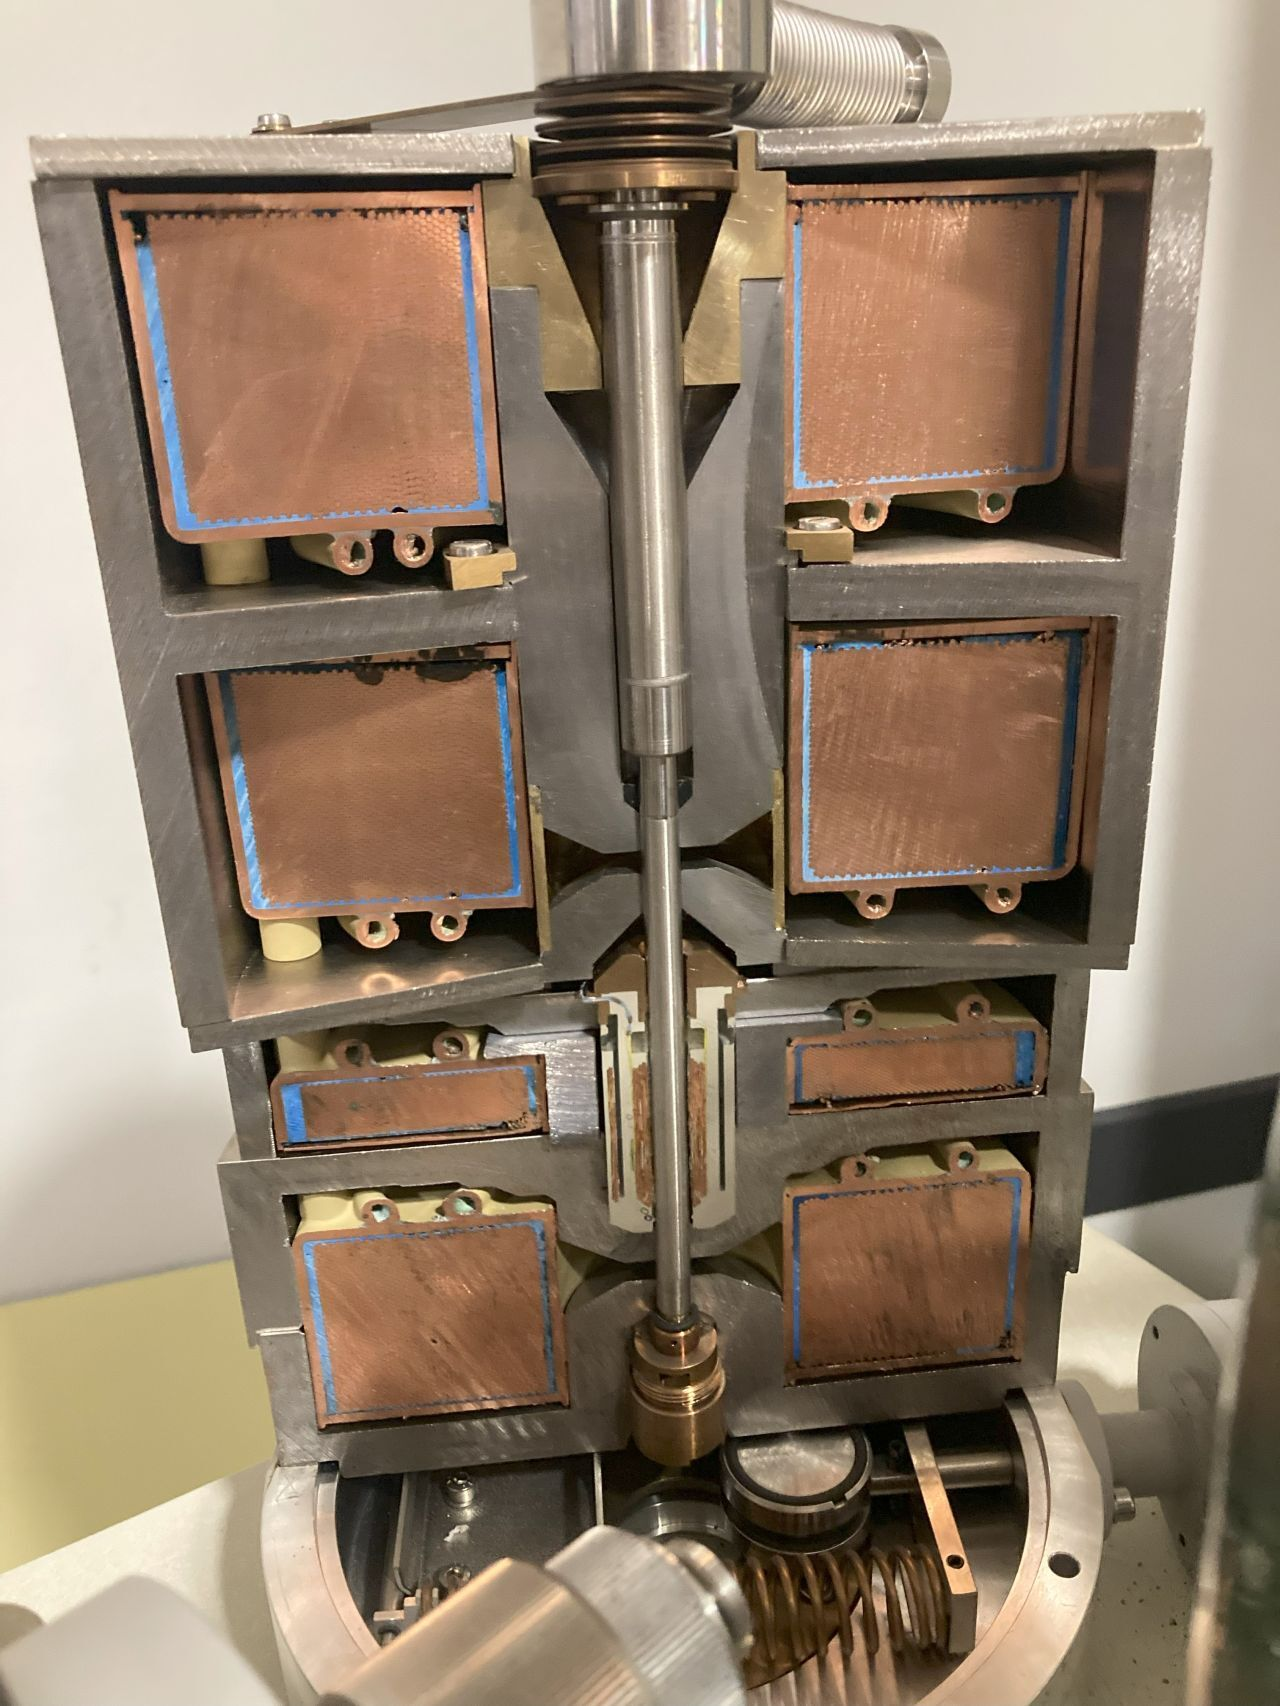
\includegraphics[width=0.5\linewidth]{Images/Phillips_CrossSection.jpg}
    \caption{Doorsnede van een Philips CM200 transmissie-elektronenmicroscoop. In een typische elektronenlens maakt men gebruik van spoelen om een magnetisch veld op te wekken. \cite{gonzalez2023}}
    \label{fig:Doorsnede_Microscoop}
\end{figure}

Ook de ontwikkeling van een open-source elektronenmicroscoop blijkt een traag en moeizaam proces te zijn. Een voorbeeld hiervan is het NanoMi project, dat streeft naar een modulaire $50$~keV transmissie-elektronenmicroscoop (TEM), zoals getoond op Figuur \ref{fig:NanoMI}. Bij het verkleinen of goedkoper maken van elektronenmicroscopen botst echter men op de fundamentele beperkingen opgelegd door conventionele magnetische lenzen: de hoge prijs, het grote formaat en gewicht, en de complexe stroomvoeding maken ze ongeschikt voor een compacte, betaalbare opstelling. Open-source initatieven zoals het NanoMi project trachtten hierrond te werken, bijvoorbeeld door het gebruik van een elektrostatische Einzellens. Ook dit brengt enkele nadelen met zich mee: er is er een relatief grote voeding nodig is om een voldoende grote spanning op te wekken die de elektronen genoeg kan afbuigen, en een elektrisch veld introduceert extra chromatische aberratie doordat ze de energieverdeling van de elektronenbundel beïnvloedt.\\

Een permanente magneet lens biedt een veelbelovend alternatief. Door gebruik te maken van kleine NdFeB-magneten en ferromagnetische poolschoenen kan een sterk, ruimtelijk geconcentreerd magnetisch veld worden opgewekt zonder enige externe stroomvoorziening. Dit maakt dit type lens compact, energiezuinig, en potentieel veel goedkoper vergeleken met conventionele solenoïdelenzen. Een dergelijke lens zou dan ook een waardevolle component kunnen vormen voor de volgende generatie open-source elektronenmicroscopen. De vevaardiging van de poolschoenen is bovendien efficïent te realiseren met moderne productietechnieken. Gebruikmakend van Computer Numerical Control (CNC) machines kunnen toleranties van $\sim0.25\mathrm{mm}$ worden behaald \cite{ModusEngineering2025}. Externe CNC-services kunnen op basis van 3D-modellen met hoge precisie componenten aanleveren.\\

\begin{figure}[H]
    \centering
    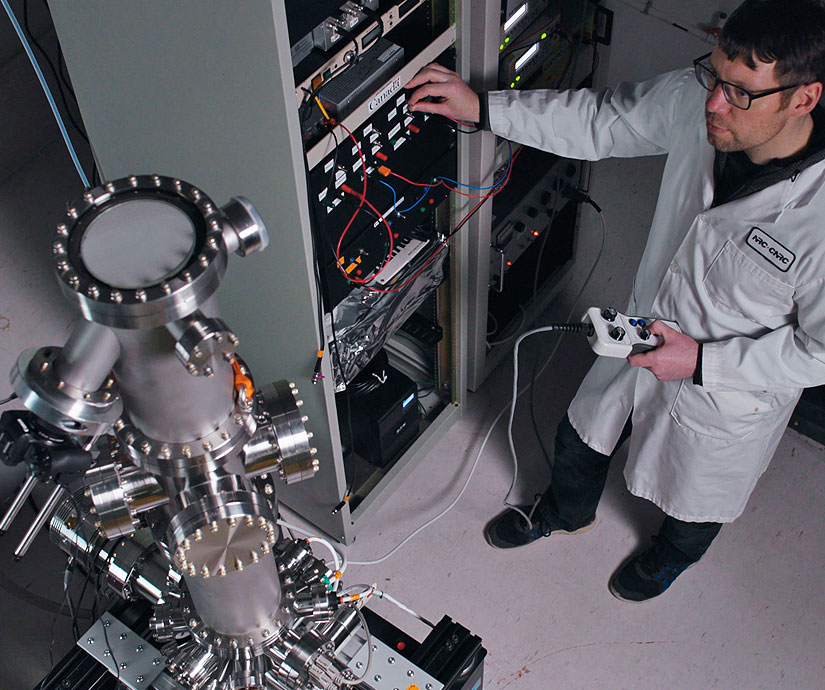
\includegraphics[width=0.5\linewidth]{Images/NanoMI.jpg}
    \caption{NanoMI is een open-source project waarbij men tracht een modulaire transmissie-elektronenmicroscoop met een versnelspanning van $50$~keV te ontwikkelen. Men gebruikt elektrostatische Einzellenzen voor het afbuigen van de elektronen. \cite{MALAC2022103362}}
    \label{fig:NanoMI}
\end{figure}

In deze thesis tracht ik een prototype van een permanente magneet lens gebaseerd op een \textit{ringvormige} NdFeB magneet te ontwerpen en realiseren m.b.v. een externe CNC-service. Deze lens zal gekarakteriseerd worden in een raster-elektronenmicroscoop met een versnelspanning van $30$~keV. Om dit ontwerp te optimaliseren, is de ontwikkeling van een Python-toolbox voor het simuleren van de lenswerking van de lens noodzakelijk. Daarnaast moeten het gesimuleerde en werkelijke lensgedrag met elkaar vergeleken worden om eventuele verschillen tussen de theoretische modellen en de fysieke realiteit te identificeren en te verklaren. De onderzoeksvraag luidt als volgt:
\vspace{5mm}
\begin{tcolorbox}[colback=gray!10!white,colframe=gray!75!black,title=Onderzoeksvraag]
    In hoeverre is het mogelijk om een miniatuur-elektronenlens bestaande op een ringvormige NdFeB en ferromagnetische poolschoenen te ontwerpen en gebruiken in een elektronenmicroscoop met een versnelspanning van $30$~keV?
\end{tcolorbox}
\vspace{5mm}

Hoofdstuk \ref{ch:literatuur} gaat dieper in op de werking van een elektronenmicroscoop en geeft een overzicht van enkele begrippen en principes die belangrijk zijn bij het ontwerpen van een elektronenlens. Hier wordt ook een afleiding  van de bewegingsvergelijking die beschrijft hoe een elekrtonenbundel wordt gefocusseerd door een cilindersymmetrisch magnetisch veld.\\

Hoofdstuk \ref{ch:methodologie} betreft de ontwikkeling van een Python-toolbox voor het simuleren van de lenswerking en het numeriek bepalen van de lenseigenschappen.\\

Hoofdstuk \ref{ch:optimalisatie} zal dieper ingaan op het toepassen van de Python-toolbox om de geometrie van de lens te optimaliseren, het vervaardigen van de lens door een CNC-service, en de experimentele karakterisering van de lens.\\

Hoofdstuk \ref{ch:vooruitzicht} bespreekt hoe het ontwerp van de lens verbeterd kan worden en hoe dit onderzoek kan bijdragen aan het ontwikkelen van een toegankelijkere open-source elektronenmicroscoop.\\

Hoofdstuk \ref{ch:besluit} geeft nog enkele laatste opmerkingen en een conclusie van dit onderzoek.\\

\chapter{Literatuurstudie}\label{ch:literatuur}
\section{Elektronenoptica}
Het oplossend vermogen van een lichtmicroscoop wordt gelimiteerd door de golflengte van het licht waarmee de beeldvorming gebeurt. De afmetingen van de kleinste details $d_{min}$ die met een optische lens kunnen worden waargenomen met een golflengte $\lambda$ is \cite{PWHawkes}:
\begin{equation}\label{eq:d_min}
    d_{min}=\frac{k\lambda}{A}
\end{equation}
Hierbij is $k$ een constante tussen $0.6-0.8$ die afhangt van de specifieke definitie van wat men als \textit{onderscheidbare} details beschouwt. $A$ is de numerieke apertuur van de lens en is gelijk aan $n_0\sin\theta_0$ met $n_0$ de brekingsindex van het meduim waaruit de lens bestaat, en $\theta_0$ de halve openingshoek van de kegel die de volledige lens belicht. Aangezien $d_{min}$ schaalt met $\lambda$ is de golflengte de beperkende factor voor de vergroting van een optische opstellingenp. Met een optische microscoop is het daardoor niet mogelijk om voorwerpen kleiner dan $\sim250\mathrm{nm}$ in beeld te brengen \cite{davidson_resolution_microscopyu}. In elektronenoptica maakt men gebruik van elektronen in plaats van fotonen om beelden te vormen. Dit laat toe om een grotere resolutie te krijgen dan met optische microscopen, aangezien voor elektronen de golflengte gegeven wordt door:
\begin{equation}
    \lambda=\frac{h}{p}=\frac{h}{\sqrt{2m_e E}}
\end{equation}
Als de elektronen vanuit rust versneld worden met een versnelspanning $\Phi$, dan krijgen ze een golflengte:
\begin{equation}
    \lambda=\frac{h}{\sqrt{2m_e e\Phi}}
\end{equation}
Door een grotere versnelspanning te gebruiken kan op deze manier kan de golflengte verder worden verkleind, wat een betere spatiale resolutie dan optische microscopen geeft. Bij HRTEM gebruikt men typisch versnelspanningen tot $300$~keV, waarmee picometer resoluties voor stabiele samples bereikt kunnen worden. Het huidige record voor de beste resolutie staat op $0.5\mathring{A}$, wat een enorme verbetering is vergeleken met de limiet voor optische microscopen \cite{Jiang2018Ptychography}. De instrumenten die nodig zijn om aan elektronenoptica te doen (zoals elektronenlenzen), zijn echter veel complexer dan hun tegenhangers die met lichtgolven beelden vormen. Een elektronenmicroscoop bestaat minstens uit een elektronenbron, een of meerdere elektromagnetische lenzen met aberratiecorrectoren, eventueel een of meerdere aperturen, en een elektronendetector. Op dezelfde manier als met licht kan een voorwerp bestraald worden met elektronen, zodanig dat de lenzen een uitvergroot beeld van dat voorwerp op de detector zullen afbeelden. Dit kan zowel in reëele ruimte, waarbij een direct beeld van eht sample verkregen wordt, als in reciproke ruimte, wat diffractiepatronen oplevert waaruit bijv. kristalstructuur en roosterparameters kunnen worden afgeleid.

\subsection{Raster/Transmissie Elektronenmicroscopie}
De twee belangrijkste vormen van elektronenmicroscopie zijn \textit{Raster Elektronenmicroscopie} (\textit{Scanning Electron Microscopy}, SEM) en \textit{Transmissie-elektronenmicroscopie} (TEM). De beeldvorming gebeurt bij beide technieken op een andere manier, en de opstellingen van de componenten in de microscoop zijn daardoor anders. In deze sectie geven we een korte beschrijving van deze twee technieken.\\

Figuur \ref{fig:SEM_principle} toont een illustratie van het werkingsprincipe van een SEM en Figuur \ref{fig:SEM_image} toont een SEM beeld van asbestos. In een SEM wordt een elektronenbundel m.b.v. elektronenlenzen in een zeer smalle spot gefocusseerd ($\sim 3\mathrm{nm}$), welke dan over het sample gescand wordt. Er wordt gebruik gemaakt van verschillende beeldvormingstechnieken afhankelijk van welke deeltjes/stralen er gemeten worden. Afhankelijk van de gedetecteerde deeltjes of straling zijn verschillende beeldvormingstechnieken mogelijk, zoals beeldvorming met \textit{terugverstrooide} elektronen (\textit{Backscattered Electrons}, BSE) of X-stralen. De meest toegepaste techniek maakt echter gebruik van secundaire elektronen (SE). De elektronenbundel zal energie uitwisselen met het sample en secundaire elektronen uit het oppervlak losslaan. Omdat de emissierichting van deze secundaire elektronen sterk afhangt van de lokale oppervlakteoriëntatie, dragen zij informatie over de driedimensionale topografie van het sample. Een elektronendetector boven het sample zal de secundaire elektronen dan verzamelen. Door de elektronenbundel met \textit{rasterspoelen} over het oppervlak te scannen, kunnen we voor elk punt op het oppervlak meten hoeveel elektronen er in de richting van de detector vrijkomen en op deze manier een beeld van het oppervlak vormen. De maximale versnelspanning van een SEM ligt typisch tussen $0.1-30$~keV \cite{PWHawkes} omdat een grotere energie te veel schade aan het sample kan opbrengen.\\

Figuur \ref{fig:TEM_principle} toont een illustratie van het werkingsprincipe van een TEM en Figuur \ref{fig:TEM_image} toont een TEM beeld van celorganellen. In een TEM zal men niet scannen over het oppervlak, maar belichten men een uiterst dun en elektronentransparant specimen (dikte van $\sim70$~nm) met een brede bundel elektronen (typisch enkele $\mu$m), welke in het ideale geval een perfecte vlakke golf voorstellen \cite{MyscopeCourse}. De elektronen zullen dan interageren met het specimen, en op sommige plaatsen meer of minder geabsorbeerd of verstrooid worden. De uitgaande elektronenbundel bevat dan opnieuw informatie over het specimen. Door gebruik te maken van een of meerdere elektronenlenzen kunnen we dan een uitvergroot beeld van het sample afbeelden op een elektronendetector die zich onder het sample bevindt. De detector is een fluorescerend scherm of een CCD camera waarop heel het beeld in 1 keer afgebeeld wordt, in tegenstelling tot het principe van een SEM. De versnelspanning in een TEM kan tot $300$~keV bedragen, waardoor de de-Brogliegolflengte van de elektronen en het oplossend vermogen aanzienlijk kleiner dan bij een SEM.

\begin{figure}[H]
    \centering
    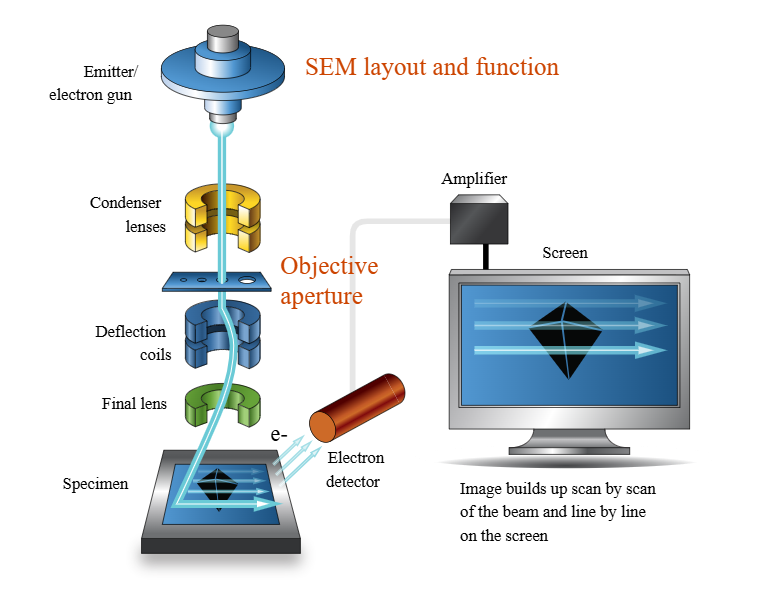
\includegraphics[width=0.7\linewidth]{Images/SEM_principle.png}
    \caption{Werkingsprincipe van een SEM waarbij de elektronenbundel over het sample wordt gescand en er secundaire elektronen los worden geslagen. \cite{MyscopeCourse}}
    \label{fig:SEM_principle}
\end{figure}

\begin{figure}[H]
    \centering
    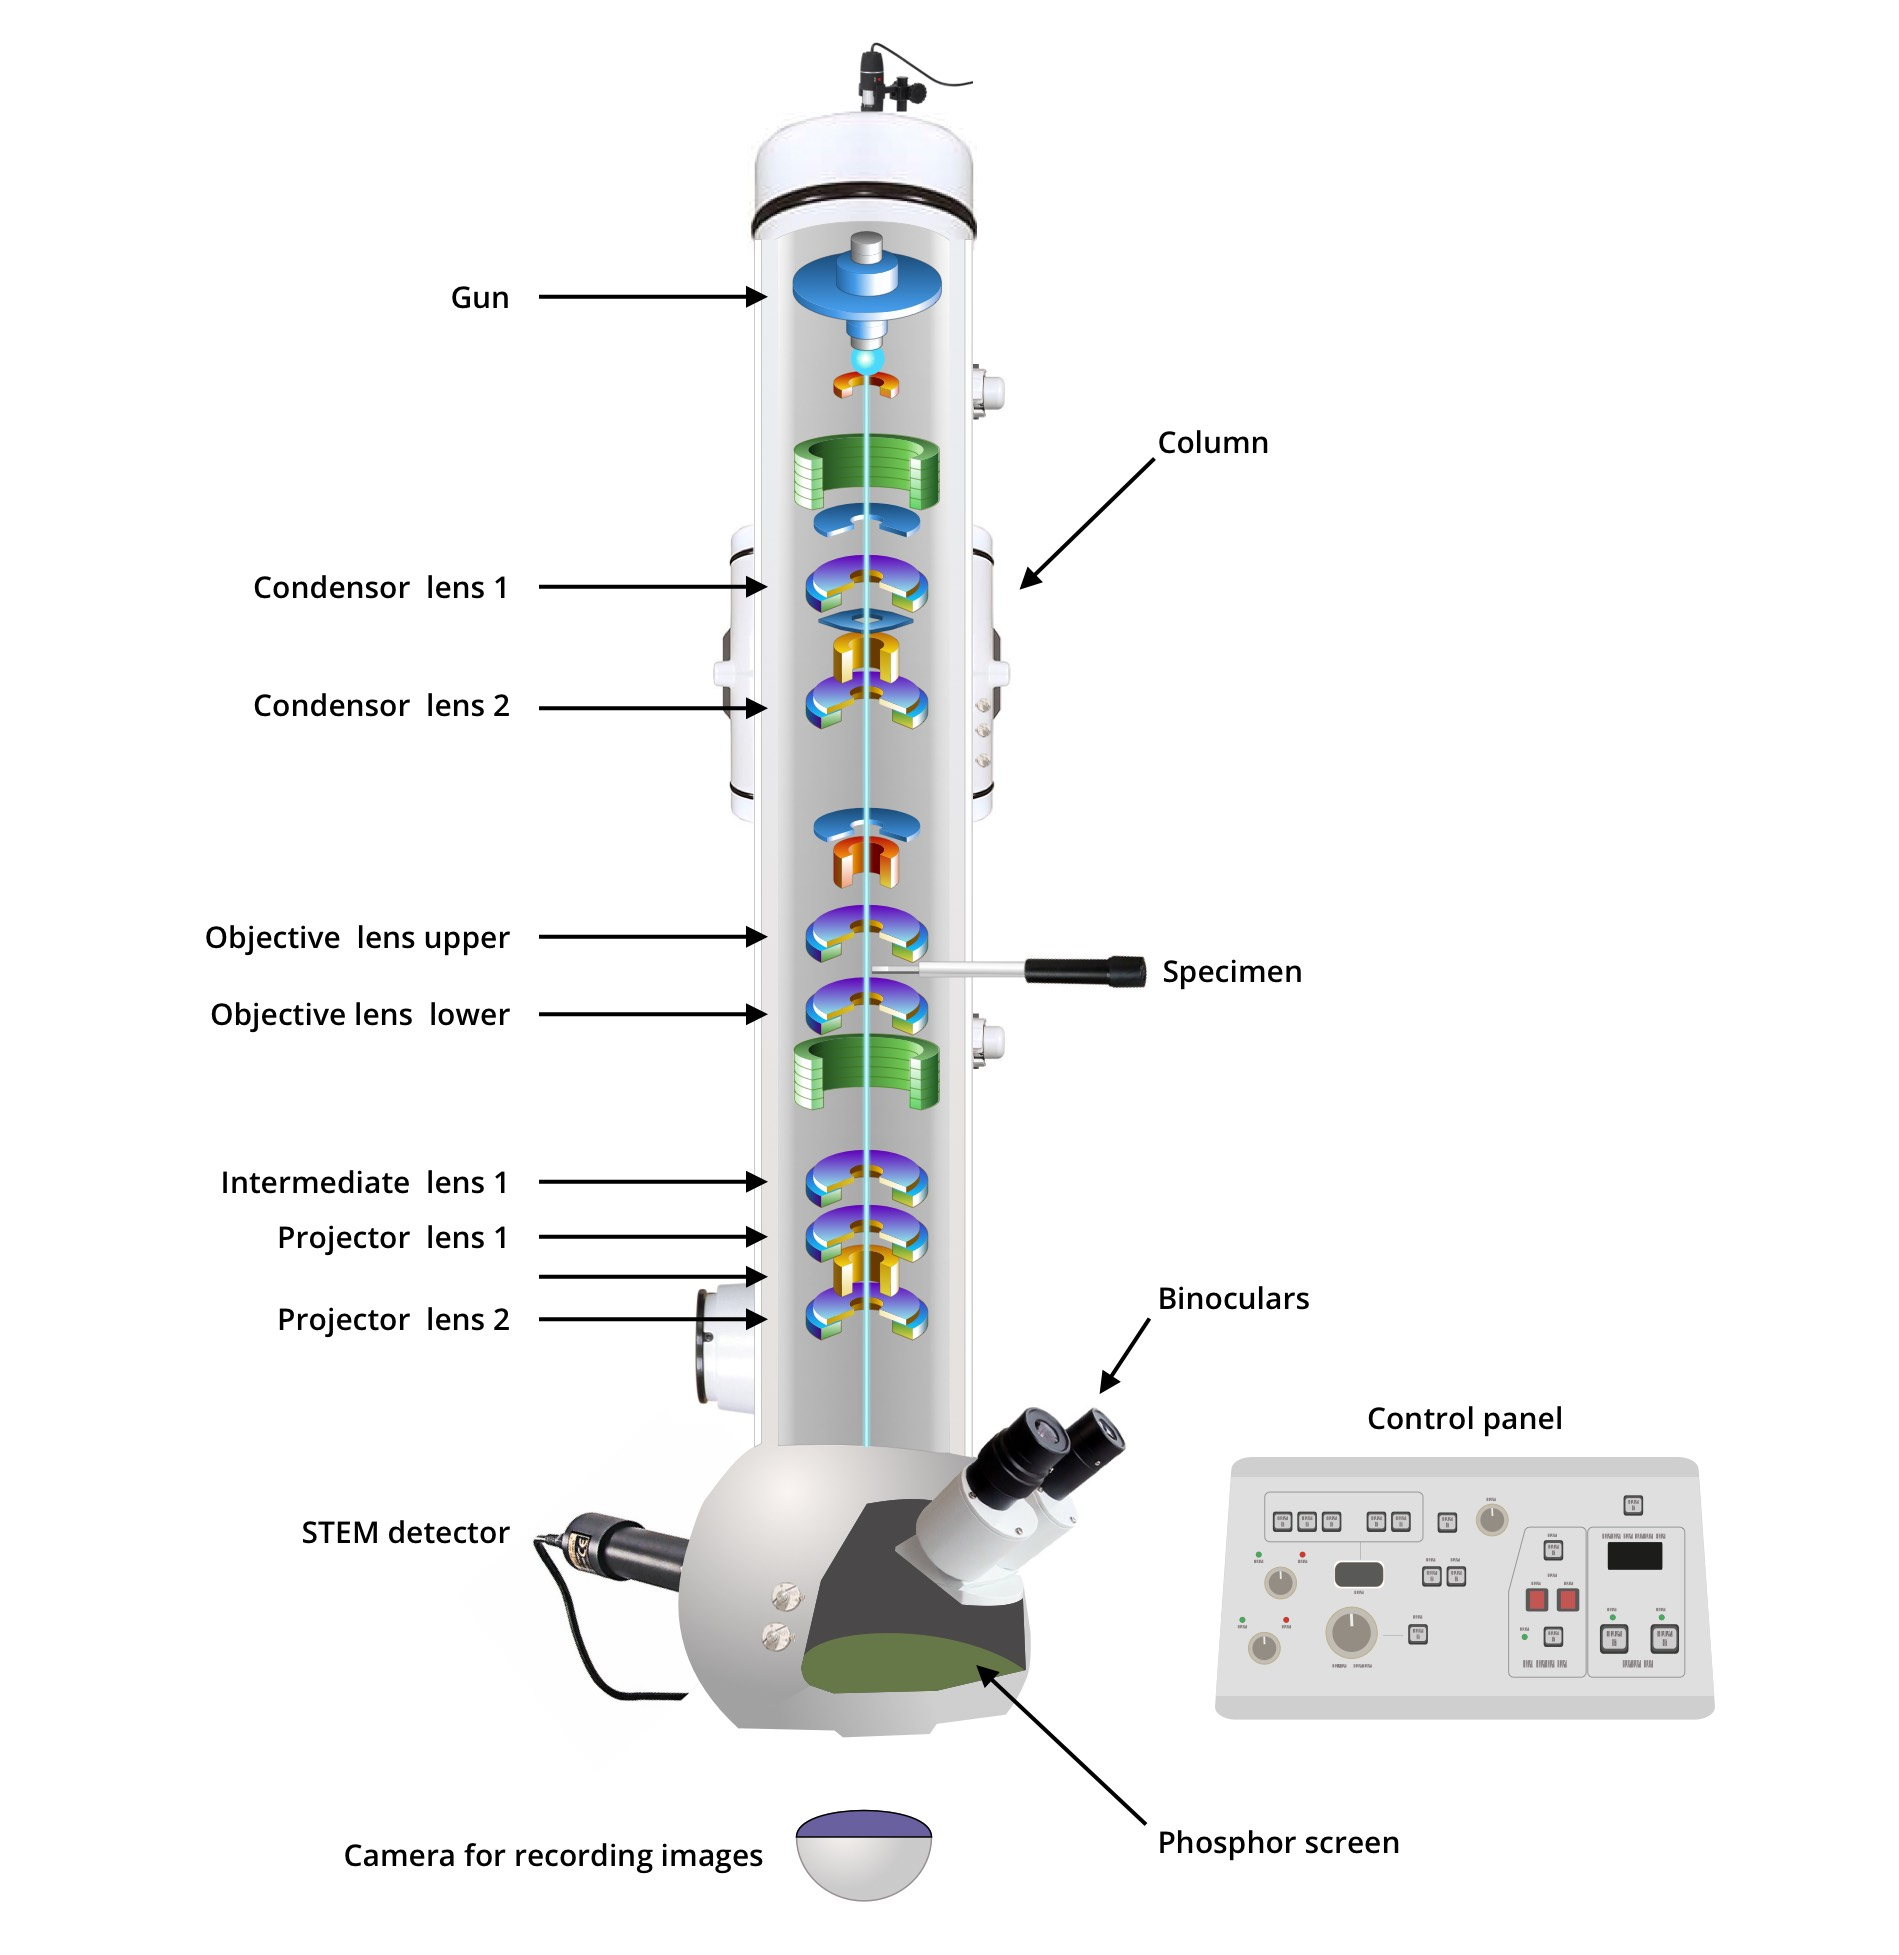
\includegraphics[width=0.8\linewidth]{Images/TEM_principle.JPG}
    \caption{Werkingsprincipe van een TEM waarbij een brede elektronenbundel heel het sample in 1 keer belicht het beeld wordt opgenomen met een detector onder het sample. \cite{MyscopeCourse}}
    \label{fig:TEM_principle}
\end{figure}

\begin{figure}[H]
    \centering
    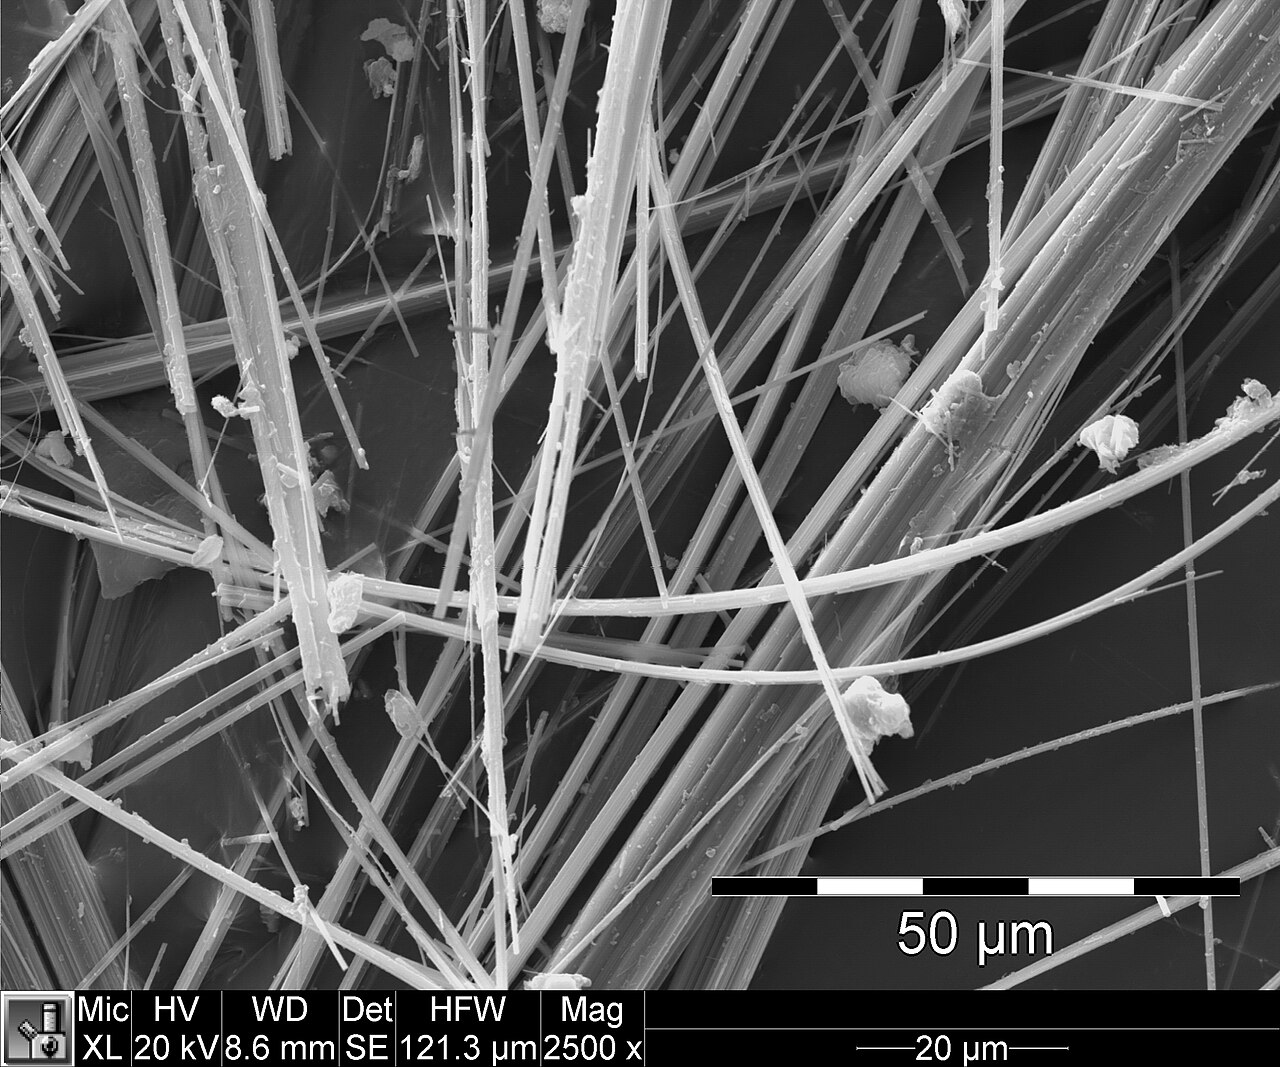
\includegraphics[width=0.6\linewidth]{Images/SEM_image.jpg}
    \caption{Beeld van asbestos opgenomen met een SEM. \cite{ravaka2011asbestos_sem}}
    \label{fig:SEM_image}
\end{figure}

\begin{figure}[H]
    \centering
    
\includegraphics[width=0.6\linewidth]{Images/TEM_image.png}
    \caption{Beeld van hematiet langs de $[001]$ as opgenomen met een TEM. \cite{klementova2021hematite_hrtem}}
    \label{fig:TEM_image}
\end{figure}



\section{Magnetische elektronenlenzen voor elektronenmicroscopie}
Om met elektronen beelden te kunnen vormen zijn elektronenlenzen een cruciale component van de opstelling. Er zijn twee manieren om een elektronenbundel te doen afbuigen: met de elektrisch veld via de Coulombkracht, en met een magnetisch veld via de Lorentzkracht. Er bestaan zowel elektrostatische als magnetische lenzen. Het gebruik van magnetische elektronenlenzen is echter veel prominenter dan elektrostatische elektronenlenzen, aangezien er zeer groote elektrische velden nodig zijn ($\sim200$~MV/m) om bij TEM versnelspanningen genoeg afbuiging van de snel bewegende elektronen te veroorzaken. Deze velden zijn praktisch niet haalbaar en veroorzaken grote veiligheidsgevaren. Bovendien zal een elektrostatische lens de energieën van de elektronen in de elektronenbundel beïnvloeden. Dit kan een spreiding van de energieën veroorzaken, wat aanleiding geeft tot chromatische aberratie (zie sectie \ref{ch:aberraties}). \cite{ElektronenLenzenGuzzinati}\\


Figuur \ref{fig:Magnetic_Electron_Lens_illustration} toont een illustratie van de manier waarop elektronen door een solenoïdelens zullen bewegen. Met een magnetische elektronenlens maakt men typisch een axissymetrisch magnetisch veld rond de optische as, waarvan de sterkte langs de optische as variëert. Vanwege de symmetrie is azimutale component van het magnetisch veld gelijk aan nul. Dit soort veld wordt opgewekt door een solenoïde waar een stroom doorheen gestuurd wordt, wat men een solenoïdelens noemt. Door een elektronenbundel door de solenoïde te sturen zullen de elektronen die zich niet op de optische as bevinden een Lorentzkracht ondergaan en afbuigen. De elektronen ondergaan zowel een radiale kracht, waarmee de bundel gefocusseerd kan worden, als een azimutale kracht, die voor een precessie van de elektronenbundel rond de optische as zorgt. In hoofdstuk \ref{ch:theorie} gaan we dieper in op de bewegingsvergelijking die het afbuigen van de elektronen beschrijft. 

\begin{figure}[H]
    \centering
    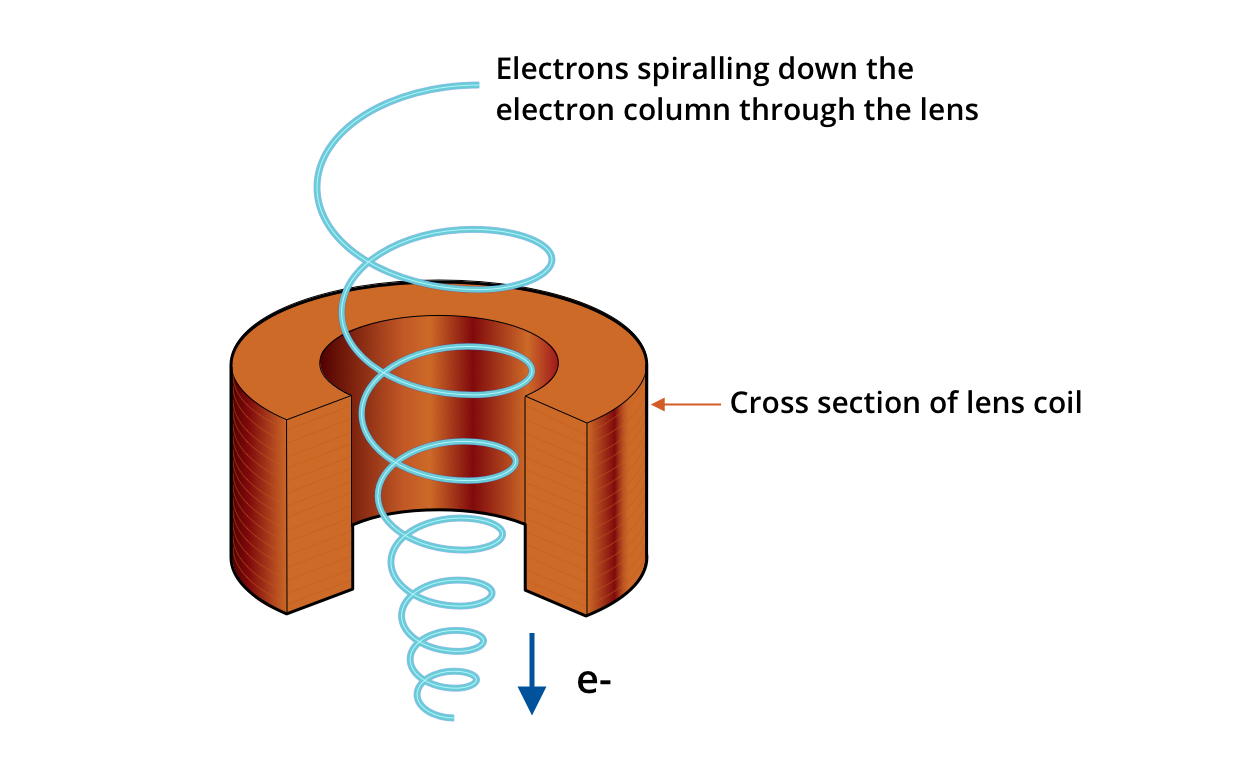
\includegraphics[width=0.7\linewidth]{Images/Magnetic_Electron_Lens_illustration.jpg}
    \caption{Illustratie van een magnetische solenoïdelens die typisch wordt gebruikt in een elektronenmicroscoop. Dit soort lens maakt een magnetisch veld dat symmetrisch is rond de optische as van het systeem. Door een bundel elektronen door de lens te sturen ondervinden deze zowel een azimutale als een radiale Lorentzkracht. De radiale component kan gebruikt worden om de elektronen te focusseren. \cite{MyscopeCourse}}
    \label{fig:Magnetic_Electron_Lens_illustration}
\end{figure}

\subsection{Condenser/objectief/projector lenzen}

\subsection{Aberraties}\label{ch:aberraties}

\subsubsection{Distortie}
\cite{PWHawkes}
\begin{equation}\label{eq:distortion}
    \begin{split}
        x_i & = M\left(x_0+Dx_0\left(x_0^2+y_0^2\right)\right)\\
        y_i & = M\left(y_0+Dy_0\left(x_0^2+y_0^2\right)\right)\\
    \end{split}
\end{equation}

\subsubsection{Chromatische aberratie}
\begin{equation}\label{eq:chr_ab}
    \begin{split}
        x_i & = M\left(x_0+C_Mx_0\frac{\Delta\Phi}{\Phi}\right)\\
        y_i & = M\left(y_0+C_My_0\frac{\Delta\Phi}{\Phi}\right)\\
    \end{split}
\end{equation}

\subsubsection{Sferische aberratie}

\section{Permanente magneet elektronenlenzen voor elektronenmicroscopie}

\section{Paraxiale beweginsvergelijking}
In deze sectie geven we een verkorte afleiding van de paraxiale vergelijking die de baan van een elektronenbundel in een axissymetrisch magnetisch veld beschrijft. De afleiding is gebaseerd op \cite{PWHawkes}. De meest algemene bewegingsvergelijking van een elektron in een elektromagnetisch veld wordt gegeven door de tweede wet van Newton waarbij de Lorentzkracht op het elektron inwerkt:
\begin{equation}\label{eq:2nd_law_newton}
    m\frac{d^2\mathbf{r}}{dt^2}=-e(\mathbf{E}+\mathbf{v}\times\mathbf{B})
\end{equation}
In ons geval beschouwen we een magnetische lens, dus stellen we het elektrostatisch veld $\mathbf{E}=\mathbf{0}$. Verder veronderstellen we dat het veld axissymetrisch is, dus is het natuurlijk om deze vergelijking in cilindercoördinaten $(r, \theta, z)$ te beschrijven. Uit de symmetrie van het systeem volgt dat de angulaire component van het magnetisch veld nul moet zijn, m.a.w. $\mathbf{B}=(B_r, 0, B_z)$. Vergelijking \ref{eq:2nd_law_newton} componentsgewijs uitrekenen geeft dan:
\begin{align}
    \mathbf{e_r}: \quad & m\left(\frac{d^2r}{dt^2}-r\left(\frac{d\theta}{dt}\right)^2\right) = -erB_z\frac{d\theta}{dt} \label{eq:2nd_law_newton_r} \\[6pt]
    \mathbf{e_\theta}: \quad & m\left(2\frac{dr}{dt}\frac{d\theta}{dt}+r\frac{d^2\theta}{dt^2}\right) = -e\left(B_r\frac{dz}{dt}-B_z\frac{dr}{dt}\right) \label{eq:2nd_law_newton_theta} \\[6pt]
    \mathbf{e_z}: \quad & m\frac{d^2z}{dt^2} = eB_r\frac{d\theta}{dt} \label{eq:2nd_law_newton_z}
\end{align}
In het linkerlid van vergelijking \ref{eq:2nd_law_newton_theta} herkennen we de Leibnizregel en kan herschreven worden als:
\begin{equation}\label{eq:theta_tussenstap}
    \frac{m}{r}\frac{d}{dt}\left(r^2\frac{d\theta}{dt}\right)=e\left(B_z\frac{dr}{dt}-B_r\frac{dz}{dt}\right)
\end{equation}
We beschouwen nu enkel paraxiale elektronen, m.a.w. elektronen die zich dicht bij de optische as van het systeem ($r=0$) bevinden. We kunnen aantonen dat $B_z(r, z)$ ontwikkeld kan worden in een reeks van machten in $r$. Stellen we $B(z)=B_z(r=0, z)$:
\begin{equation}\label{eq:b_z_expansion}
    B_z(r, z)=B(z)-\frac{r^2}{4}\frac{d^2B(z)}{dz^2}+\frac{r^4}{64}\frac{d^4B(z)}{dz^4}+O(r^6)
\end{equation}
Voor kleine $r$ maken we de benadering dat $B_z(r, z)=B(z)$. Nu leiden we een relatie tussen $B$ en $B_r$ af. We beschouwen een cilindrisch volume rond de z-as van het systeem zoals op Figuur \ref{fig:maxwell_2_cilinder} en gebruiken de tweede Maxwellvergelijking in integraalvorm, welke ons vertelt dat de totale flux doorheen een gesloten ondervlak gelijk moet zijn aan $0$.
\begin{figure}[H]
    \centering
    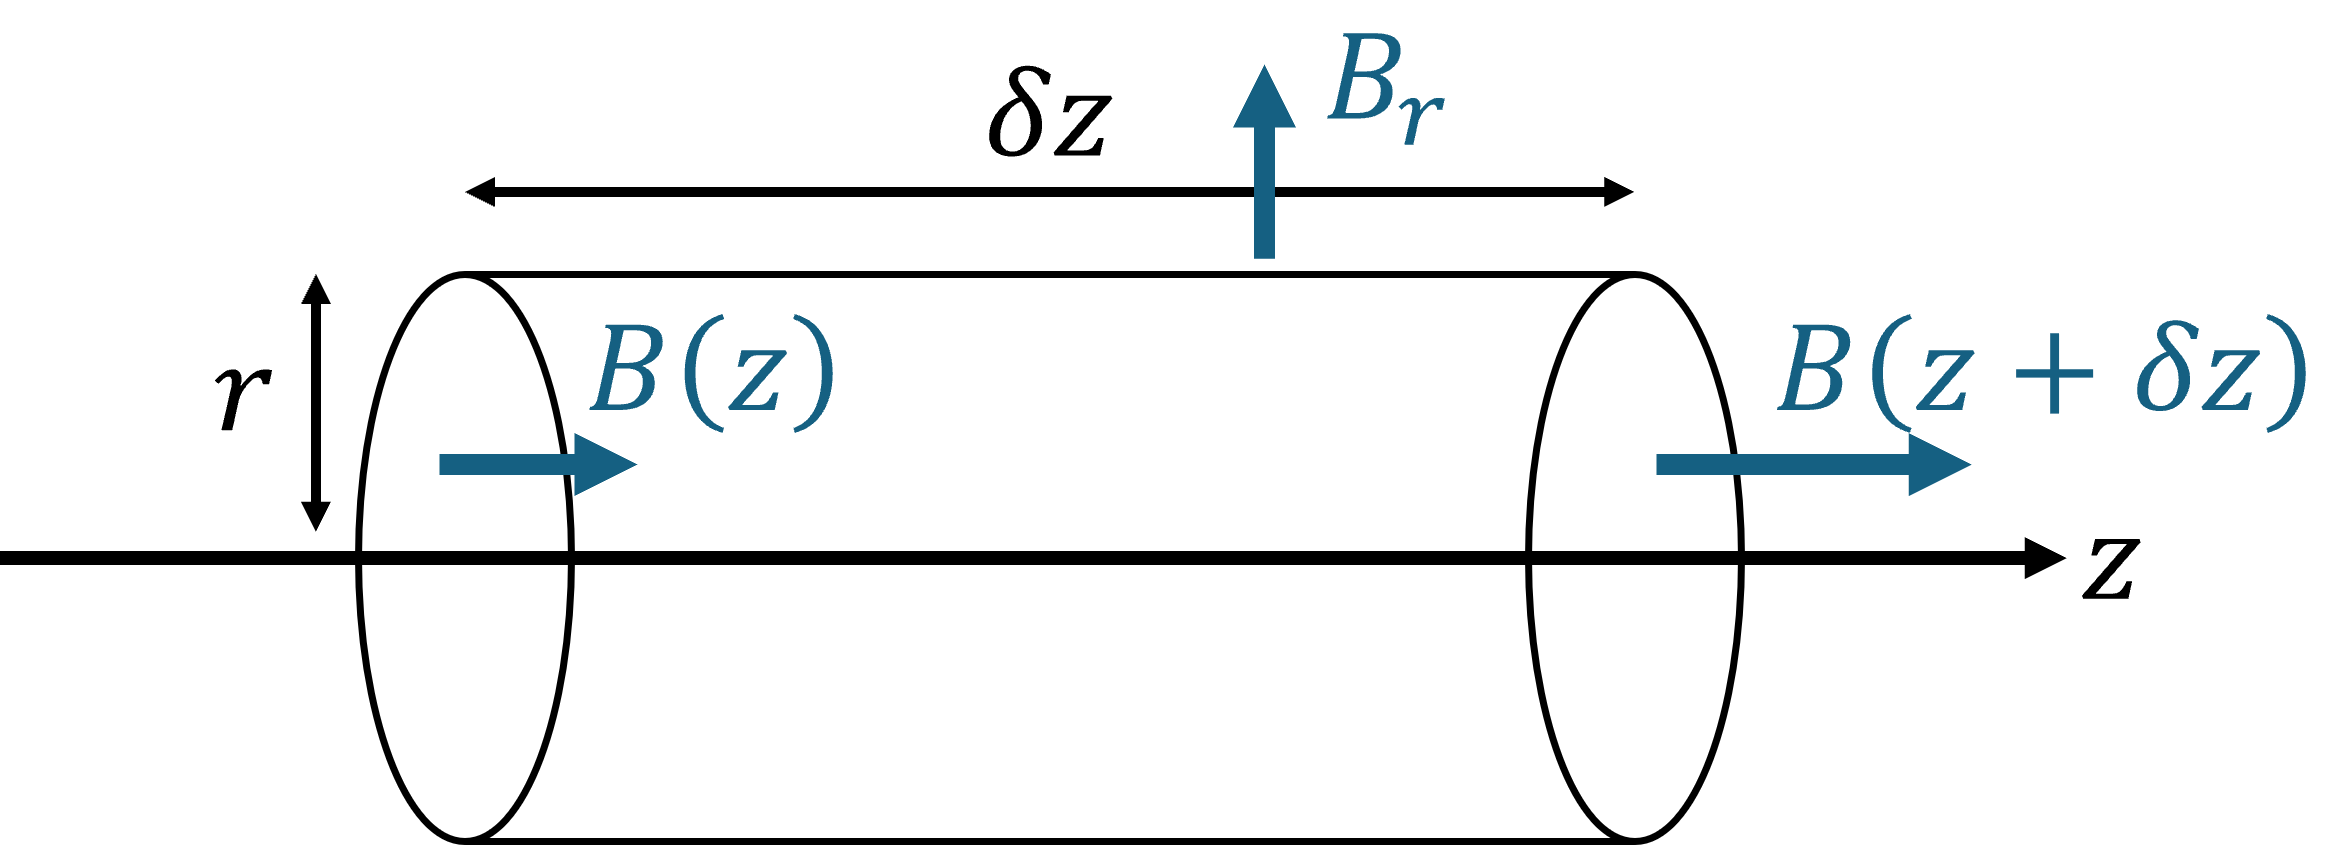
\includegraphics[width=0.5\linewidth]{Images/maxwell_2_cilinder.png}
    \caption{We kunnen de tweede Maxwell gebruiken om een relatie te vinden tussen $B_r$ en $B(z)$ op de symmetrie-as van het systeem. We tekenen daarvoor een cilindervormig Gauss-oppervlak waardoor de totale flux $\int\mathbf{B}\cdot d\mathbf{S}$ moet verdwijnen.}
    \label{fig:maxwell_2_cilinder}
\end{figure}
De flux doorheen de mantel wordt gegeven door $2\pi r\delta zB_r$, terwijl de flux doorheen het boven-en ondervlak gegeven wordt door $\pi r^2(B(z+\delta z)-B(z)\approx\pi r^2\frac{dB}{dz}$. Hieruit volgt:
\begin{equation}\label{eq:Br_Bz_relation}
    \int_S\mathbf{B}\cdot d\mathbf{S}=\pi r^2\frac{dB}{dz}+2\pi r\delta zB_r=0\Leftrightarrow B_r=-\frac{1}{2}r\frac{dB}{dz}
\end{equation}
Invullen van \ref{eq:Br_Bz_relation} in \ref{eq:theta_tussenstap} geeft:
\begin{equation}
    \frac{d}{dt}\left(mr^2\frac{d\theta}{dt}\right)=er\left(B\frac{dr}{dt}+\frac{1}{2}r\frac{dB}{dz}\frac{dz}{dt}\right)=\frac{d}{dt}\left(\frac{1}{2}er^2B\right)
\end{equation}
Beide leden integreren\footnote{In principe moet hier nog een constante $+C$ bij, maar aangezien $\frac{d\theta}{dt}=0$ bij $\mathbf{B}=0$ is $C=0$.} en vereenvoudigen geeft:
\begin{equation}\label{eq:precession}
    \frac{d\theta}{dt}=\frac{eB}{2m}=\eta^2B
\end{equation}
met $\eta=\sqrt{\frac{e}{2m}}\approx3\times10^5\sqrt{\frac{Q}{kg}}$ voor elektronen. We kunnen nu vergelijking \ref{eq:precession} invullen in vergelijking \ref{eq:2nd_law_newton_r}:
\begin{equation}\label{eq:paraxialevgl_dt}
    \frac{d^2r}{dt^2}=-r\frac{e^2B(z)^2}{2m^2}+r\frac{e^2B(z)^2}{4m^2}=-\eta^4B(z)^2r
\end{equation}
Nu willen we nog de variabele $t$ vervangen door $z$ om zo een gewone differentiaalvergelijking in 1 variabele te krijgen. Stel dat we werken met een versnelspanning $\Phi$, dan geldt er wegens behoud van energie dat:
\begin{equation}
    \frac{1}{2}m\left(\frac{dz}{dt}\right)^2=e\Phi\Leftrightarrow\frac{dz}{dt}=\sqrt{\frac{2e\Phi}{m}}=2\eta\sqrt{\Phi}
\end{equation}
Waaruit volgt:
\begin{equation}
    \frac{d^2}{dt^2}=4\eta^2\Phi\frac{d^2}{dz^2}
\end{equation}
Door dit in te vullen in \ref{eq:paraxialevgl_dt} komen we uiteindelijk bij de paraxiale bewegingsvergelijking voor axissymetrisch magnetisch veld:
\begin{equation}\label{eq:paraxialevgl}
    \frac{d^2r}{dz^2}+\frac{\eta^2B(z)^2}{4\Phi}r=0
\end{equation}
De relativistisch correcte versie van deze vergelijking is:
\begin{equation}\label{eq:paraxialevgl_rel}
    \frac{d^2r}{dz^2}+\frac{\eta^2B(z)^2}{4V}r=0
\end{equation}
Met $V=\Phi\left(1+\frac{e}{2mc^2}\Phi\right)$. Voor een versnelspanning van $30$~keV is dit een correctie van $2.93\%$. Deze vergelijking moet numeriek opgelost worden voor het geschatte magnetisch veld om de lenseigenschappen van lens te simuleren. \\

Merk op dat de paraxiale bewegingsvergelijking lineair is. Dit betekent dat twee lineair onafhankelijke oplossingen voldoende is om de algemene oplossing van deze vergelijking op te stellen. Conventioneel noemt men $z_0$ de positie van het vlak van het voorwerp dat we met een magnetische lens willen uitvergroten, en kiest met twee basisoplossingen $g(z)$ en $h(z)$ zodanig dat:
\begin{align}\label{eq:gh}
    g(z_0)=1, g'(z_0)=0 \\[6pt]
    h(z_0)=0, h'(z_0)=1
\end{align}
Merk op dat de oplossing $g$ het gedrag van een parallelle bundel beschrijft. Immers, de oplossing voor de paraxiale bewegingsvergelijking van een parallel elektron dat initieel op een constante afstand $r_0$ van de optische as beweegt kan geschreven worden als $r_0g(z)$. Stel dat $g(z)$ een nulpunt heeft, dan kruisen alle initieel parallel bewegende elektronen de optische as in dat nulpunt. Dit is exact de gewenste werking van een magnetische elektronenlens; het nulpunt van $g(z)$ is dan het brandpunt van de lens. Vergelijking \ref{eq:paraxialevgl_rel} lijkt erg op een harmonische oscillator (met een frequentie afhankelijk van $B^2$), wat betekent dat de elektronen steeds naar de optische as worden afgebogen. In het algemeen zal $g(z)$ daarom altijd een nulpunt hebben als $B(z)\neq0$.7

\section{Reële/Asymtotische lenseigenschappen}
Bij het berekenen van de lenseigenschappen is het belangrijk om een onderscheid te maken tussen de reële en asymptotische lenseigenschappen. Wanneer we meerdere lenzen in een opstelling gebruiken, zijn het namelijk de asymptotische lenseigenschappen die we nodig hebben om de afstanden tussen de lenzen en de vergroting te berekenen. Een voorbeeld wordt getoond op Figuur \ref{fig:reeel_asymtotic} waarbij we de reëele en asymptotische focale lengte vergelijken.

\begin{figure}[H]
    \centering
    
\includegraphics[width=0.75\linewidth]{Images/reeel_asymptotisch.png}
    \caption{Voorbeeld van het verschil tussen een reëele en een asomptotische lenseigenschap. In dit geval is de reëele focale lengte het punt waar de elektronenbaan $g$ de optische as kruist, en de asymptotische focale lengte het punt waar de asymptoot rakend aan $g$ voor $z\rightarrow\infty$ de optische as kruist.}
    \label{fig:reeel_asymtotic}
\end{figure}

De focale lengte wordt gevonden door te bepalen waar een parallel inkomende straal de otpische as van het systeem snijdt. In dit geval zijn er echter twee stralen die kunnen worden beschouwd, waardoor er ook twee focale lengtes te definiëren zijn:
\begin{itemize}
    \item De reëele focale lengte is het punt waar een parallelle elektronenbundel op de optische as gefcousseerd wordt. Dit is met andere woorden het nulpunt van $g(z)$.
    \item De asymptotische focale lengte is het punt waar de asymptoot voor $z\rightarrow\infty$ aan $g$ de optiche as kruist. Als we een parallelle bundel op de lens insturen, lijkt het voor een observator die achter van het midden van de lens staat alsof de elektronen niet uit het reëel, maar het asymptotisch brandpunt komen. Ook wanneer we een beeld gaan vormen met een beeldafstand dir groot is vergeleken met $f$, moeten we de asymptotische focale lengte gebruiken om de vergroting te berekenen. De asymptotische focale lengte is daarom voor onze doeleinden de relevante waarde.
\end{itemize}

\color{red} 
Extra sectie met uitleg waarom we best meer dan 1 lens nodig hebben om een diffractiepatroon uit te vergroten?\\
Meer uitleg over wat een hoofdvlak is? 
\color{black}

\chapter{Methodologie afschatting lensparameters}\label{ch:methodologie}
Om een het ontwerp voor een werkende elektronenlens te realiseren moeten de geometrische dimensies van de lens zorgvuldig worden vastgelegd. Deze afmetingen zijn cruciaal, aangezien ze de vorm en het profiel van het magnetisch veld op de optische as bepalen, welke de lenswerking en lenseigenschappen vastleggen. De invloed van de \textit{lensparameters} op de lenswerking moet daarom vooraf gesimuleerd kunnen worden. Deze parameters omvatten de binnen en buitenstralen van de poolschoenen en de magneet, de dikte van de magneet, de dikte van de luchtspleet tussen de poolschoenen, en het remanent magnetisch veld van de lens. Dit vereist zowel een analytisch model van het magnetisch veld als een numerieke methode om de baanvergelijkingen van de elektronen op te lossen. De volgende objectieven worden opgesteld:
\begin{tcolorbox}[colback=red!10!white,colframe=red!75!white,title=Objectief 1]
    Het ontwerpen van een lensgeometrie met een permanente magneet en ferromagnetische poolschoenen die een voldoende sterk gelokaliseerd magnetisch veld in het midden van de lens veroorzaakt om de elektronen af te buigen.
\end{tcolorbox}

\begin{tcolorbox}[colback=red!10!white,colframe=red!75!white,title=Objectief 2]
    Het opstellen van een analytische uitdrukking $B(z)$ op voor de grootte van het magnetisch veld volgens de $z$-as op de optische as van de lens in functie van de lensparameters. Deze uitdrukking mag benaderend zijn, maar moet de lenseigenschappen zo accuraat mogelijk kunnen voorspellen.
\end{tcolorbox}

\begin{tcolorbox}[colback=red!10!white,colframe=red!75!white,title=Objectief 3]
    Het kwantificeren van de invloed van het demagnetiserend veld, veroorzaakt door de oppervlakken van de poolschoenen, op de effectieve veldsterkte in de magneet. Dit effect hangt af van de lensparameters, rekening houdend met de $\mathrm{BH}$-curve van de magneet.
\end{tcolorbox}

\begin{tcolorbox}[colback=red!10!white,colframe=red!75!white,title=Objectief 4]
    Het ontwikkelen van een Python-toolbox om de werking van de lens te simuleren. Deze toolbox moet het volgende functionaliteiten combineren:
    \begin{enumerate}
        \item Het magnetisch veld $B(z)$ voor een bepaalde geometrie van de lens berekenen op basis van de gevonden analytische uitdrukking.
        \item De paraxiale bewegingsvergelijking voor een willekeurig magnetisch veld $B(z)$ numeriek oplossen om de lenseigenschappen te bepalen.
        \item Analytische uitdrukkingen voor de distortie en chromatische aberratiecoëfficiënten numeriek evalueren door integralen met de analytische uitdrukking voor $B(z)$ en haar afgeleiden numeriek uit te rekenen.
    \end{enumerate}
\end{tcolorbox}

\section{Opbouw en principe permanente magneetlens}
Voor we in de details van het ontwerpsproces van de lens duiken, is het verstandig om het concept van het ontwerp helder uit te leggen. Het doel is om een magnetisch veld te ontwerpen dat de elektronen op zo'n manier afbuigt zodanig dat een paralelle bundel geconcentreerd zal worden in een punt op de optische as. Hierbij willen we dat de lens aan enkele gewenste eigenschappen voldoet.\\

\begin{enumerate}
    \item Ten eerste willen we een geschikte focale lengte zodat de lens bruikbaar is in een elektronenmicroscoop. Concreet zal deze lens getest worden in een Tescan MIRA SEM, waarin we een maximale totale afstand van $228.4\mathrm{mm}$ van elektronenbron tot detector ter beschikking hebben. Om een bruikbare lens te maken is het daarom gewenst dat de focale lengte niet veel langer dan $10\mathrm{mm}$ is. Verder zullen we werken we met een versnelspanning van $30$~keV, wat een voorwaarde legt op de minimale sterkte van het magnetisch veld. \\

    \item Ten tweede is het gewenst dat de lens die we maken, een dunne lens is. Meer concreet willen we dat de hoofdvlakken samenvallen in het midden van de lens. Op deze manier is het gemakkelijker om berekeningen te doen als we opstellingen met meerdere lenzen willen bouwen, aangezien de dunne lensformule dan toepasbaar is. Dit betekent dat we een sterk ruimtelijk geconcentreerd magnetisch veld in het midden van de lens willen; de elektronen interageren dan maar heel kort met het magnetisch veld, wat een dunne lenswerking geeft. Hoe geconcentreerder we het veld maken, hoe sterker het maximale veld moet zijn om dezelfde afbuiging te veroorzaken. Om een bruikbare lens te maken willen we op de optische as een magnetisch veld met een sterkte van $\sim0.1-1\mathrm{T}$ dat geconcentreerd is over een afstand van $<5\mathrm{mm}$. \\
\end{enumerate}

Het ontwerp dat in deze thesis onderzocht wordt en aan beide voorwaarden voldoet, wordt getoond op Figuur \ref{fig:lens_circuit_diagram}.
\begin{figure}[H]
    \centering
    
\includegraphics[width=0.6\linewidth]{Images/lens_circuit_diagram.png}
    \caption{Doorsnede van het ontwerp van onze permanente magneetlens. Een homogeen gemagnetiseerde Nd-ringmagneet maakt een sterk magnetisch veld dat door twee zacht magnetische poolschoenen wordt geconcentreerd in het  het gat van de lens.}
    \label{fig:lens_circuit_diagram}
\end{figure}

Om een axissymetrisch veld te veroorzaken, maken we gebruik van een kleine ringvormige NdFeB magneet met een remanent magneetveld van $\sim1.2\mathrm{T}$. We kunnen in principe enkel de magneet als lens gebruiken, maar dit is niet optimaal; het magnetisch veld zou dan te homogeen in de ruimte zijn, terwijl we een zo sterk mogelijk veld op de symmetrieas van de lens willen. We kunnen het veld naar het midden van de lens 'begeleiden' d.m.v. poolschoenen gemaakt uit een zacht ferromagnetisch materiaal met een hoge permeabiliteit $\mu$. Als de permabiliteit voldoende hoog is, dan zullen de grote meerderheid van de veldlijnen in de poolschoenen blijven en in het midden van de lens de opening of \textit{luchtspleet} oversteken. Bij het oversteken van de opening tussen de poolschoenen lopen de velden niet perfect loodrecht van het ene oppervlak naar het andere, maar door randeffecten zullen ze naast de oppervlakken naar buiten buigen. Op deze manier krijgen we in het gat een lokaal sterk veld, zoals gewenst.\\

% Voor de ringmagneet kiezen we een NdFeB van graad N35. Er bestaan magneten met betere graden, maar voor een relatief kleine versnelspanning van $30$~keV is dit materiaal voldoende sterk. Voor de poolschoenen gebruiken ASI1018, een zacht ferromagnetisch staal dat geschikt is om gebruikt te worden in een CNC-machine. Deze materialen zullen meer in detail besproken worden in sectie \ref{ch:lensontwerp}.\\

\begin{tcolorbox}[colback=blue!10!white,colframe=blue!75!black,title=Realisatie objectief 1]
    Een permanente magneet lens kan gerealiseerd worden met een ontwerp waarbij een NdFeB ringmagneet gecombineerd wordt met axissymetrische poolschoenen. Dit vormt een magnetisch veld dat geconcentreerd wordt in de luchtspleet tussen de poolschoenen, waardoor de elektronen zeer kort interageren met dit magnetisch veld.
\end{tcolorbox}

\section{Analytische afschatting magnetisch veld}
Vooraleer we de lenseigenschappen van de lens kunnen simuleren, willen we een analytische schatting maken van het magnetisch veld $B(z)$ op de symmetrieas van de lens. Hiervoor maken enkele belangrijke benaderingen om de berekeningen te vereenvoudigen.\\

\begin{enumerate}
    \item Ten eerste veronderstellen we dat de magnetische veldlijnen volledig in de poolschoenen zullen blijven tot ze de luchtspleet tussen de poolschoenen bereiken, zonder dat er magnetisch veld op andere plaatsen naar buiten lekt. We zorgen ervoor dat dit een goede benadering blijft door de geometrie van de poolschoenen zo te ontwerpen dat het magnetisch veld nergens anders kan kortsluiten. We willen met andere woorden dat er geen andere paden $C$ van de bovenkant naar de onderkant van de ringmagneet mogelijk zijn die een een kleinere/gelijkaardige reluctantie $\mathcal{R}=\int_C\frac{dl}{\mu(l)A(l)}$ hebben. Daarnaast zorgen we ervoor dat de poolschoenen gladde en afgeronde oppervlakken hebben om randeffecten te voorkomen, aangezien magnetische veldlijnen de neiging hebben om zich te concentreren rond oppervlakken met een kleine kromtestraal, zoals randen en hoeken.\\

    Om wiskundig te beschrijven waar de magnetische velden de poolschoenen verlaten of weglekken, is het gemakkelijk om gebruik te maken van magnetische poolladingen. De magnetische lading aan het oppervlak van een gemagnetiseerd volume wordt gegeven door $\sigma_M=\mathbf{M}\cdot\mathbf{n}$ met $\mathbf{M}$ de magnetisatie van het materiaal en $\mathbf{n}$ een normaalvector op het oppervlak. In het ideale geval zijn de poolschoenen zo gemagnetiseerd dat de magnetisatie altijd parallel ligtaan de zijoppervlakken ligt zodat $\sigma_M=0$. Alleen bij de oppervlakken die aan de luchtspleet grenzen staat de magnetisatie loodracht op het oppervlak, waardoor we daar wel een poollading krijgen. In deze benadering hebben de poolschoenen dus enkel oppervlakteladigen aan de luchtspleet tussen de poolschoenen.\\

    \item Een tweede belangrijke veronderstelling is dat de poolladingen aan de oppervlakken in de luchtspleet homogeen verdeeld zijn. Dit is een goede benadering als we een homogeen ferromagnetisch materiaal en een homogeen gemagnetiseerde ringmagneet gebruiken. De oppervlakken van de ringmagneet kunnen we immers ook als homogeen geladen oppervlakken beschouwen. De magnetische veldlijnen afkomstig van het magneetoppervlak zullen zich min of meer uniform doorheen de poolschoenen voortplanten zodat ook de luchtspleet-oppervlakken homogeen geladen zijn. Op deze manier wordt het magnetisch veld gereduceerd tot het veld veroorzaakt door twee homogeen geladen \textit{annula}\footnote{Een annulus is een oppervlak opgespannen tussen twee concentrische cirkels.} met een tegengestelde, maar even grote magnetische poollading $\pm\sigma_M$.\\
\end{enumerate}

Aan de hand van dit vereenvoudigd model kunnen we een analytische uitdrukking voor het magnetisch veld op de symmetrie-as terugvinden. We beginnen met 1 homogeen geladen annulus met een oppervlaktelading\footnote{Voorlopig kiezen we een arbitraire oppervlaktelading, in een latere sectie zullen we bespreken hoe we de juiste waarde voor $\sigma_M$ kiezen.} $+\sigma_M$ die zich rond de $z$-as op een hoogte $z=0$ bevindt. De annulus heeft een binnenstraal van $R_1$ en een buitenstraal $R_2$. Natuurlijk is het niet mogelijk om een magnetische monopool zoals in dit systeem te maken, maar dit is slechts een tussenstap: later zullen we een tweede annulus met tegengestelde lading toevoegen. Dit systeem wordt getoond op Figuur \ref{fig:analytic_expression_1_ring}.

\begin{figure}[H]
    \centering
    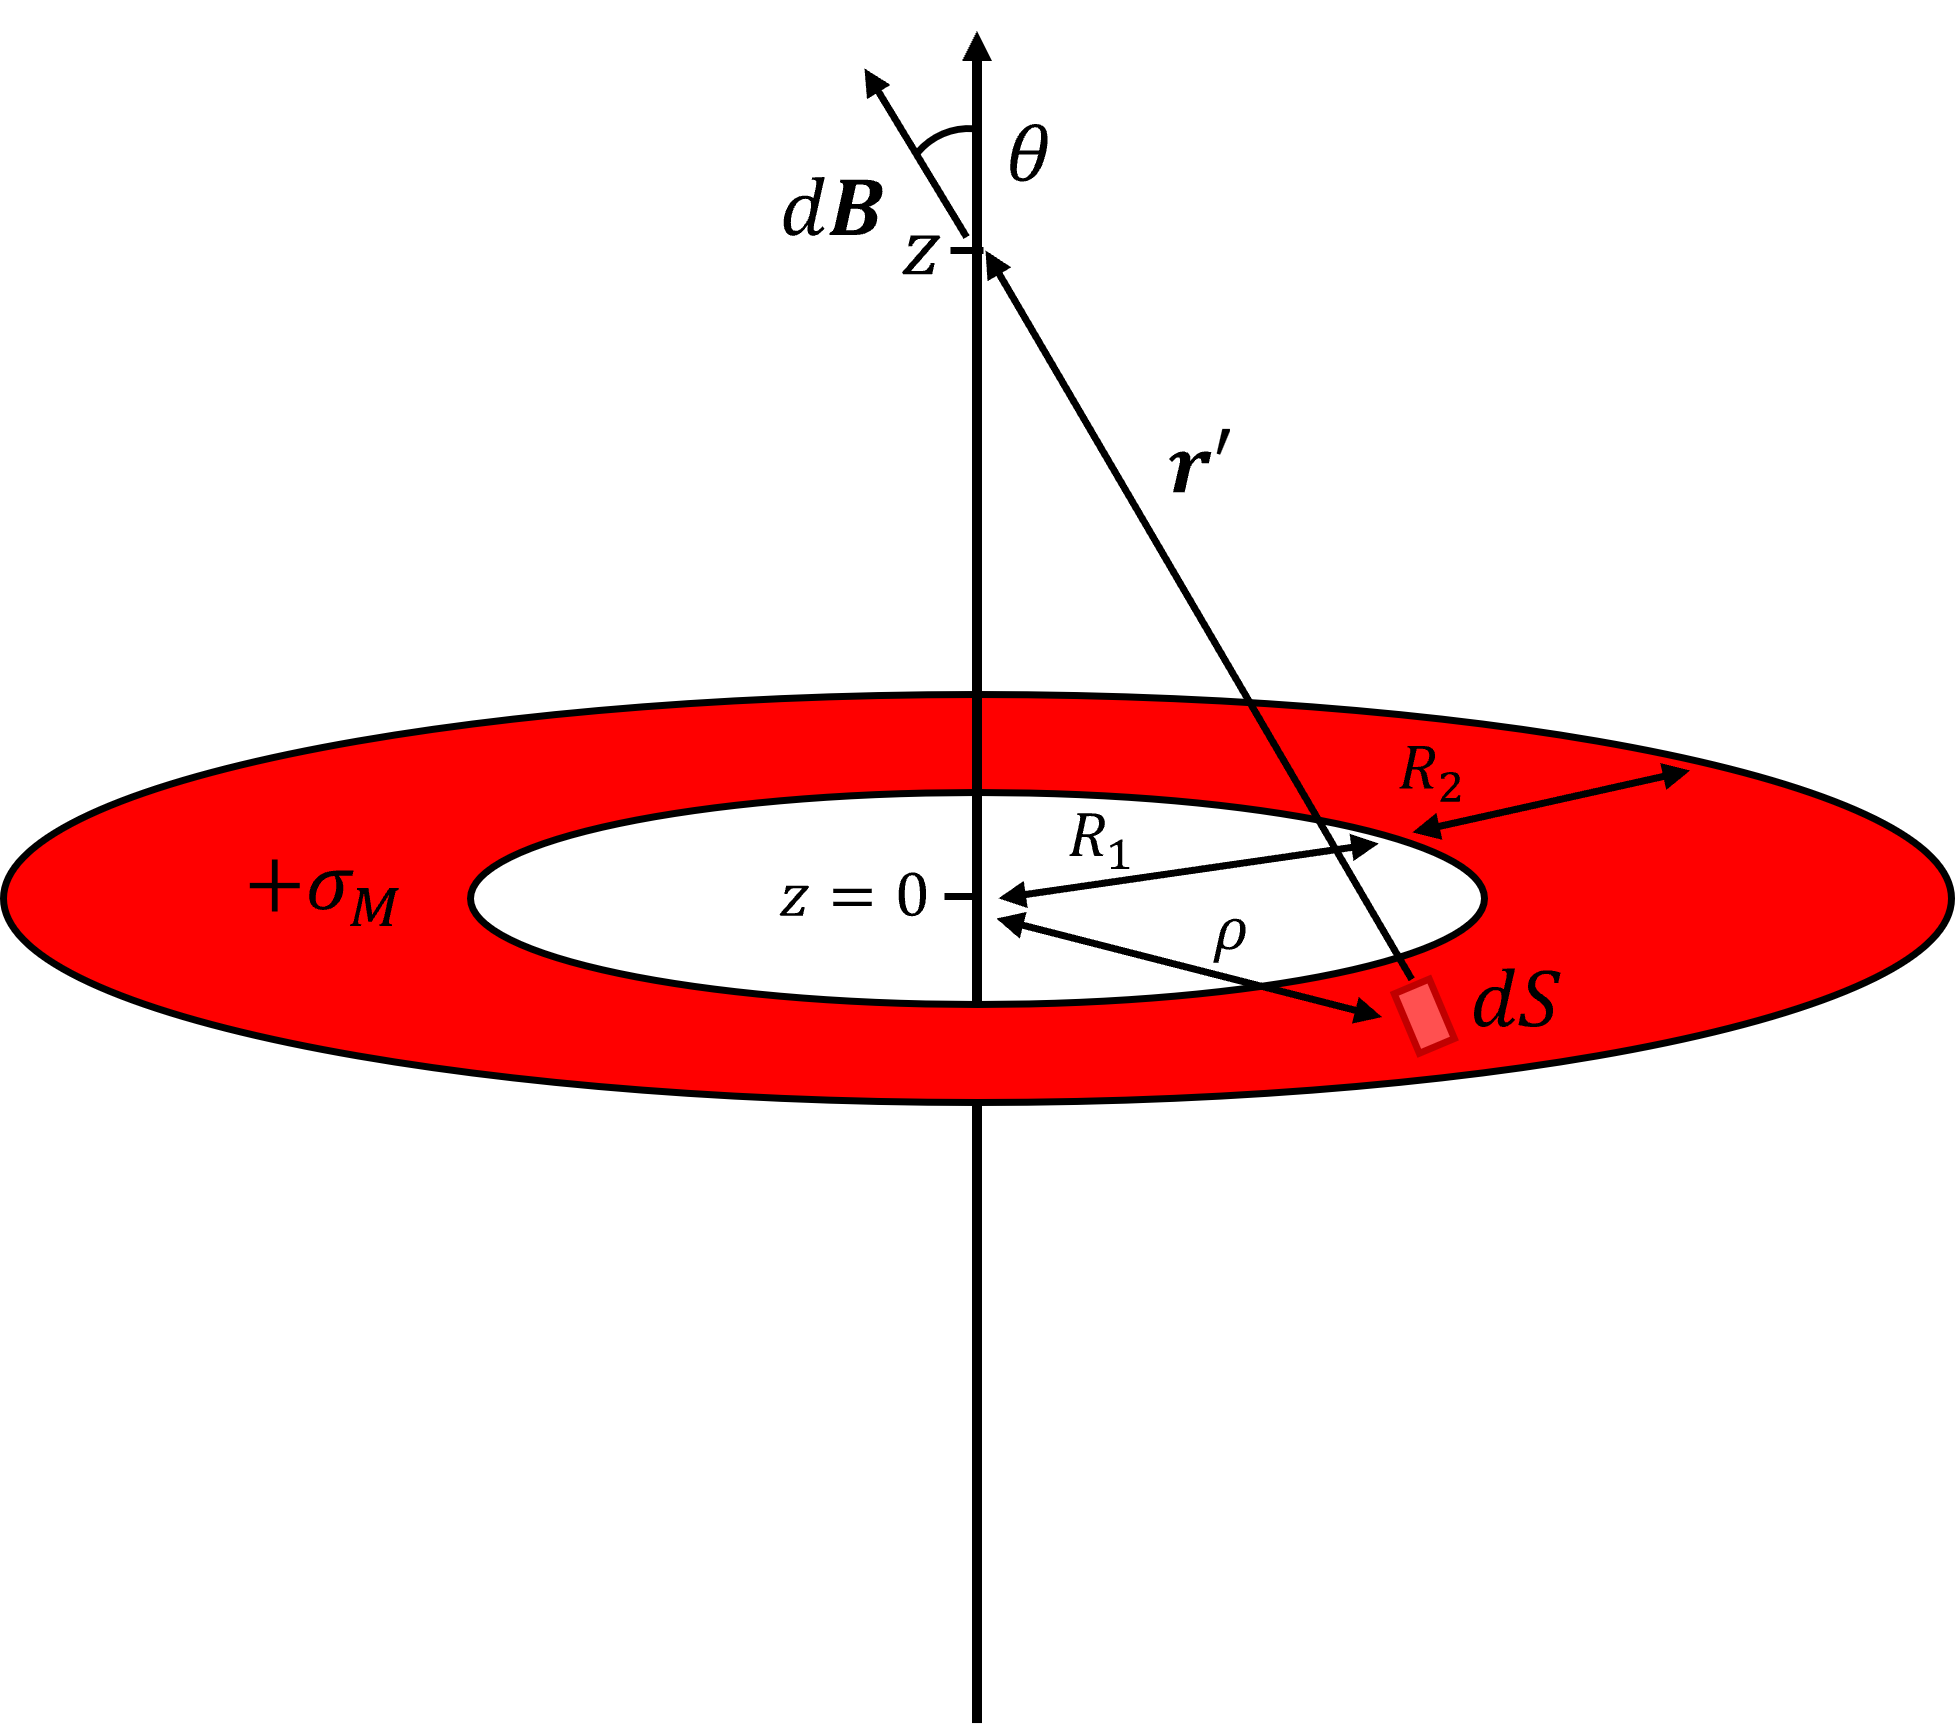
\includegraphics[width=0.5\linewidth]{Images/analytic_expression_1_ring.png}
    \caption{Systeem met 1 annulus rond een symmetrie-as. De annulus heeft een homogene oppervlaktepoollading gelijk aan $\sigma_M$, wat aanleiding geeft tot een magnetisch veld.}
    \label{fig:analytic_expression_1_ring}
\end{figure}

Het magnetisch veld in een bepaald punt $\mathbf{r}$ kan nu bepaald worden door de bijdragen van alle opeprvlakte-elementen van de annulus te integreren, net zoals we zouden doen in het elektrostatisch geval. We moeten enkel de permittiviteit $\epsilon$ vervangen door de permeabiliteit $\mu$. In ons geval zijn we enkel geïnteresseerd in het veld op de $z$-as, aangezien we in de paraxiale benadering zullen werken. Uit symmetrieoverwegingen kunnen we al zeggen dat enkel de component parallel met de $z$-as zal overblijven. We integreren de bijdragen van elk oppervlakte-elementje $dS$ op de annulus aan het resulterend magnetisch veld, dit resulteert in de volgende berekening:
\begin{equation} \label{eq:1_annulus}
\begin{split}
B_{ring}(z) & = \int_S\mathbf{e}_z\cdot d\mathbf{B} = \int_S\cos \theta\frac{ \mu_0\sigma_M}{4\pi|\mathbf{
r}'|^2}dS =  \frac{\mu_0\sigma_M}{4\pi}\int_S\frac{\cos \theta}{|\mathbf{r}'|^2}dS\\
& = \frac{\mu_0\sigma_M}{4\pi}\int_S\frac{\frac{z}{\sqrt{z^2+\rho^2}}}{z^2+\rho^2}dS = \frac{\mu_0\sigma_M}{4\pi} \int_0^{2\pi}d\phi \int_{R_1}^{R_2}\rho d\rho \frac{z}{(z^2+\rho^2)^{\frac{3}{2}}}\\
& = \frac{\mu_0\sigma_Mz}{2}\int_{R_1}^{R_2}\frac{\rho}{(z^2+\rho^2)^{\frac{3}{2}}}d\rho \quad \left(\text{Stel } u = z^2+\rho^2,\ du = 2\rho\, d\rho\right)\\
& = \frac{\mu_0\sigma_Mz}{4}\int_{z^2+R_1^2}^{z^2+R_2^2}u^{-\frac{3}{2}}du = \frac{\mu_0\sigma_Mz}{2}\left[-u^{-\frac{1}{2}}\right]_{z^2+R_1^2}^{z^2+R_2^2}\\
& = \frac{\mu_0\sigma_Mz}{2} \left(\frac{1}{\sqrt{z^2+R_1^2}}-\frac{1}{\sqrt{z^2+R_2^2}}\right)
\end{split}
\end{equation}
Op Figuur \ref{fig:B_field_1_annulus} tonen we een plot van $B_{ring}$ voor parameters $R_1=1$ en $R_2=2$. Zoals we zouden verwachten uit de symmetrie van het systeem is het veld 0 in het midden van de ring. Vlak boven en onder de ring neemt het veld sterk toe in de zin weg van de ring, aangezien veldlijnen weg van positieve/noordelijke poolladingen bewegen. Onder de ring is het veld negatief, aangezien we de $z$-as als positieve richting hebben gekozen. Ver weg van de ring kunnen we de ladingsverdeling als een puntlading beschouwen en valt het veld af als $\frac{1}{z}$.
\begin{figure}[H]
    \centering
    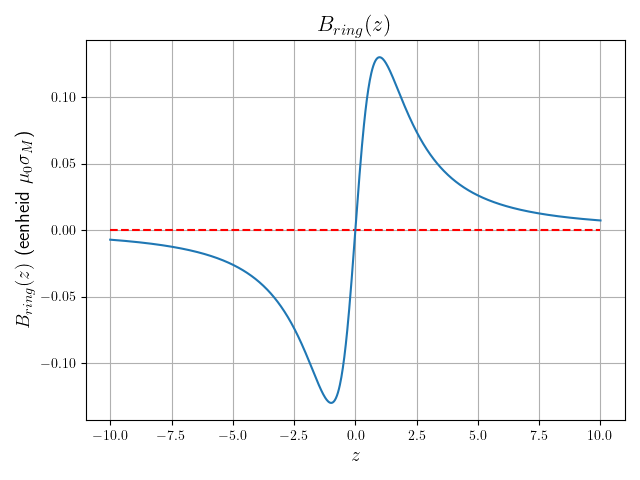
\includegraphics[width=0.6\linewidth]{Images/B_field_1_annulus.png}
    \caption{Plot van $B_{ring}$ volgens vergelijking \ref{eq:1_annulus} voor parameters $R_1=1$ en $R_2=2$. Het veld is antisymmetrisch rond het midden van de ring, zoals men zou verwachten.}
    \label{fig:B_field_1_annulus}
\end{figure}
Door te werken met poolladingsdichtheden kunnen we nu eenvoudig het veld met twee tegengesteld geladen ringvormige oppervlakken berekenen. We kunnen simpelweg een superpositie maken van twee velden veroorzaakt door een enkel oppervlak, aangezien elektromagnetische velden lineair zijn. Het systeem dat we nu beschrijven wordt getoont op Figuur \ref{fig:analytic_expression_2_rings}

\begin{figure}[H]
    \centering
    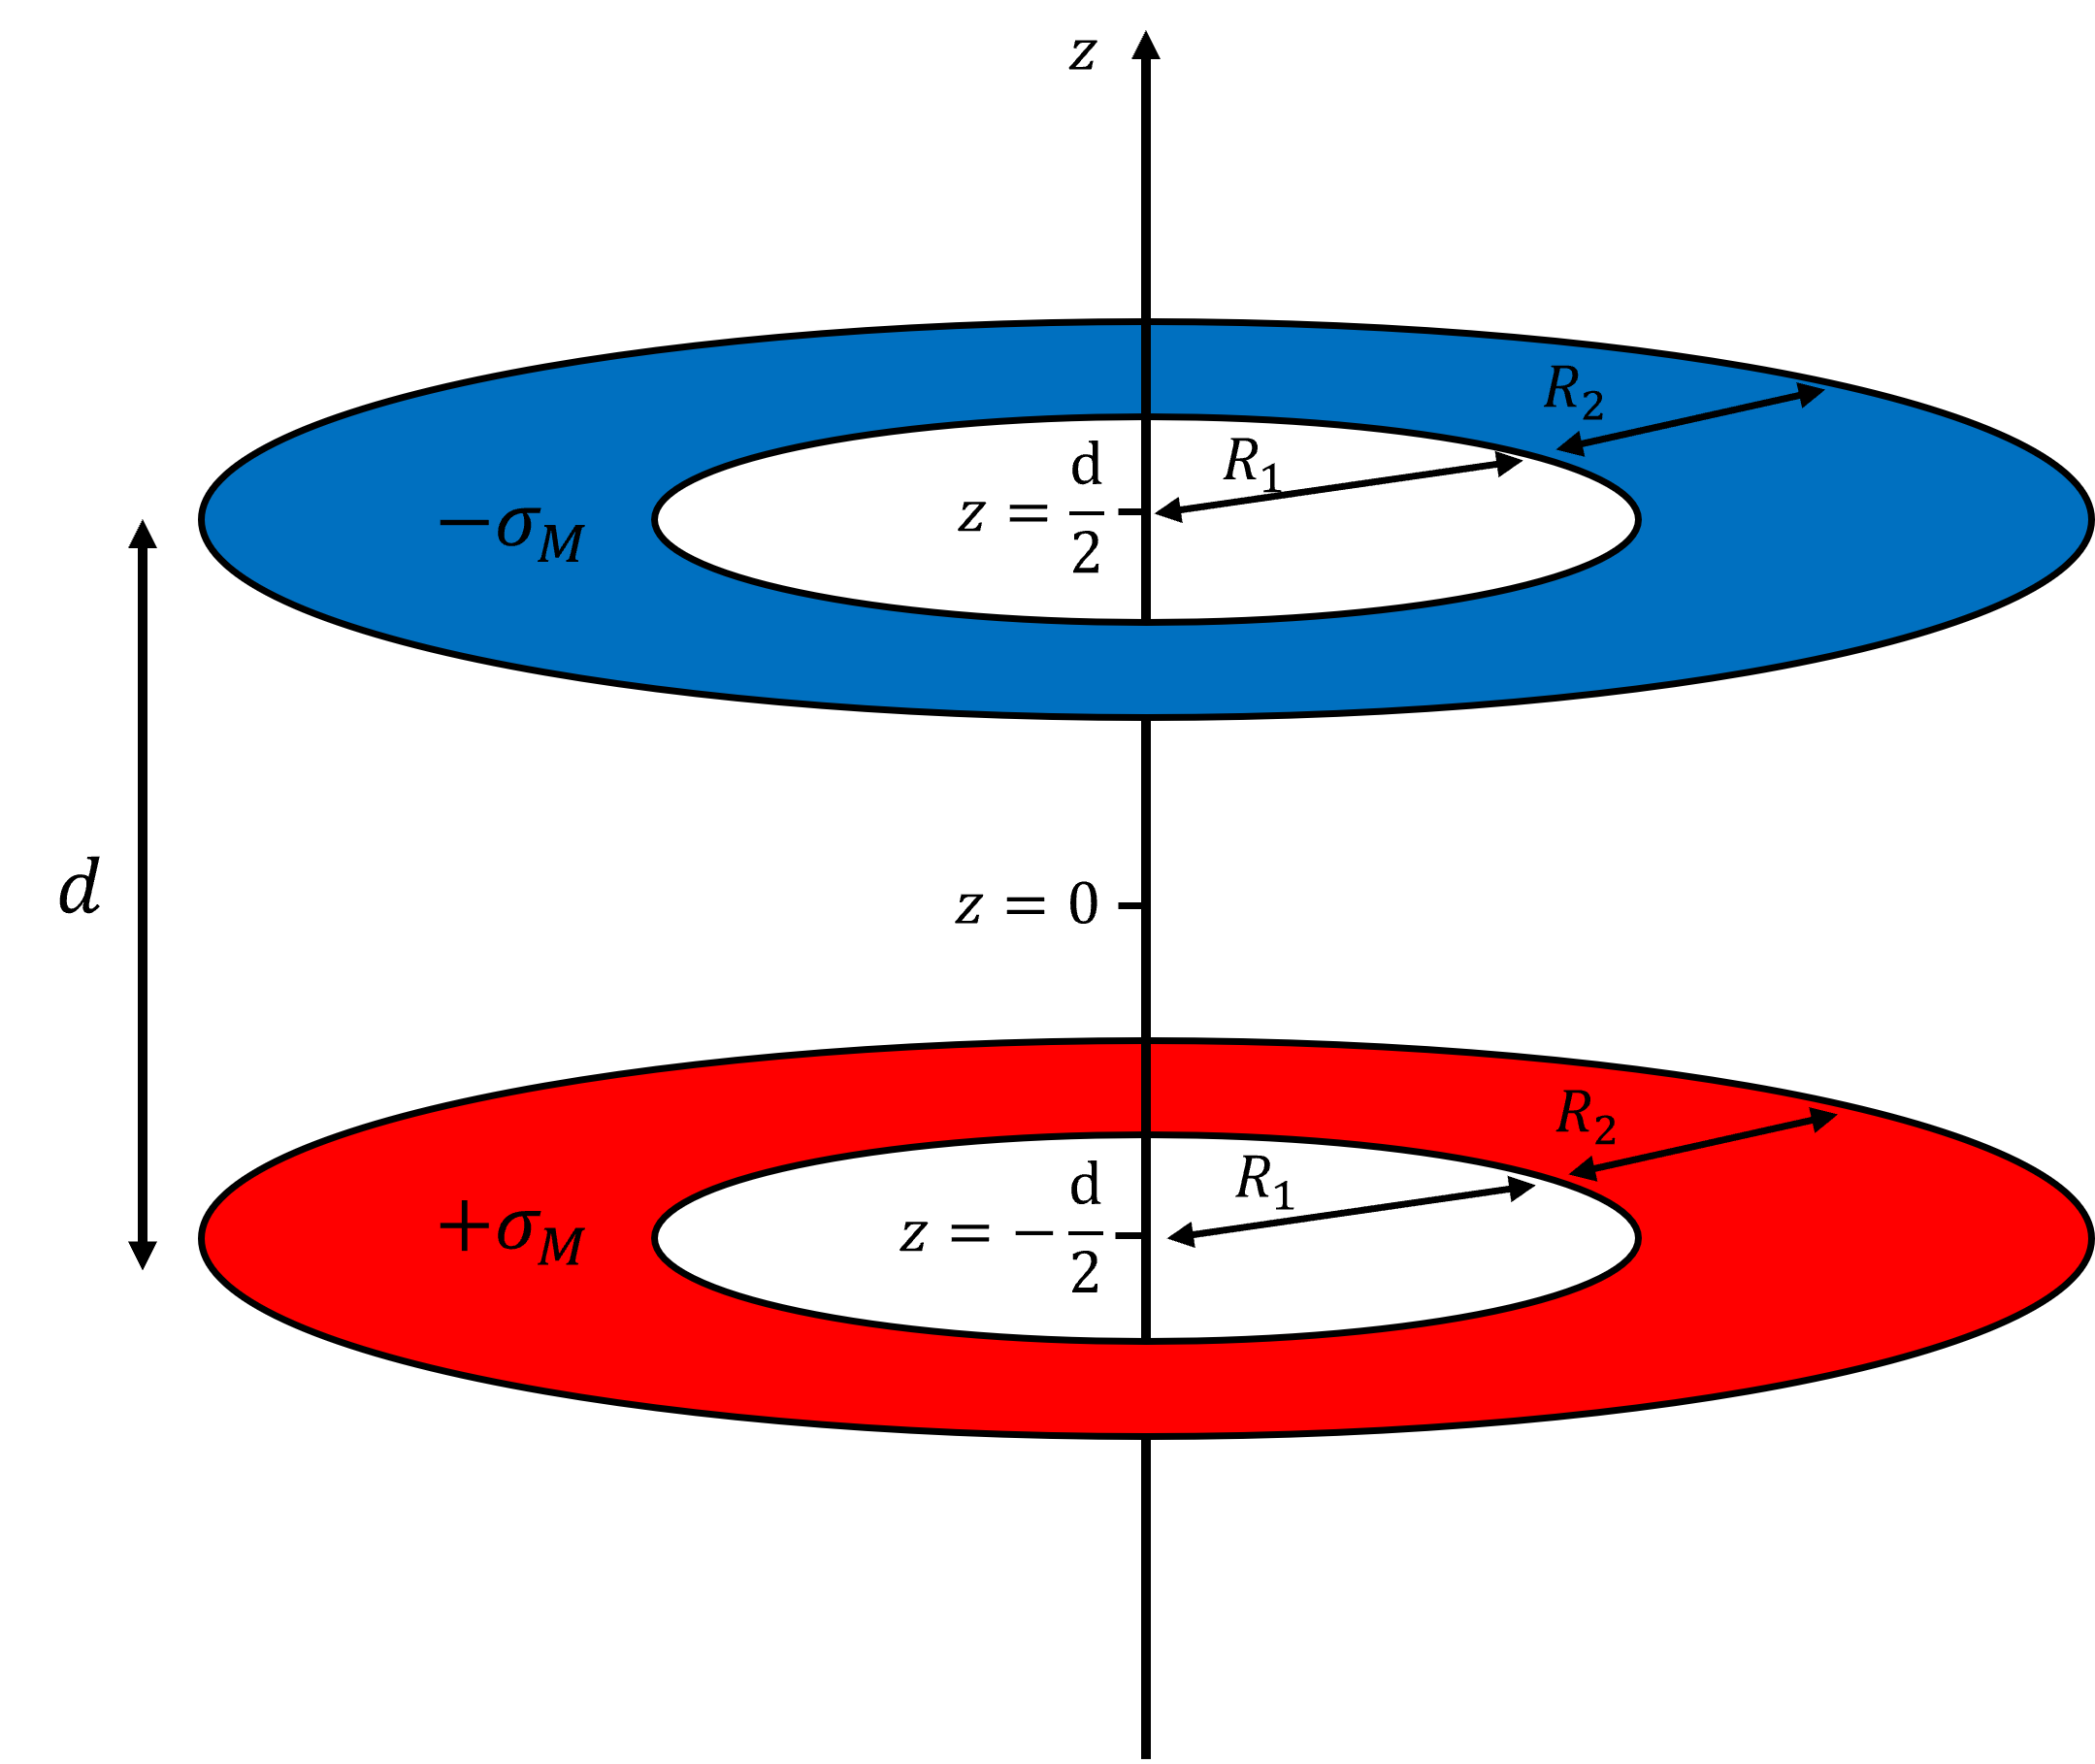
\includegraphics[width=0.45\linewidth]{Images/analytic_expression_2_rings.png}
    \caption{Systeem met 2 annula met een luchtspleetbreedte van $d$ rond een symmetrie-as. De annula hebben homogene oppervlaktepoolladingen gelijk aan $\pm\sigma_M$, wat aanleiding geeft tot een magnetisch veld. Dit is het systeem dat we beschouwen bij het afschatten van het magnetisch veld in onze lens.}
    \label{fig:analytic_expression_2_rings}
\end{figure}

Het magnetisch veld wordt nu gegeven door:
\begin{equation}\label{eq:2_annula}
\begin{split}
    B(z) &= B_{ring}\!\left(z+\frac{d}{2}\right) - B_{ring}\!\left(z-\frac{d}{2}\right) \\[8pt]
         &= \frac{\mu_0\sigma_M}{2}\biggl[
              \left(z+\frac{d}{2}\right)\biggl(
                \frac{1}{\sqrt{\bigl(z+\frac{d}{2}\bigr)^2+R_1^2}}
                - \frac{1}{\sqrt{\bigl(z+\frac{d}{2}\bigr)^2+R_2^2}}
              \biggr) \\
         &\phantom{{}= \frac{\mu_0\sigma_M}{2}\biggl[}
              - \left(z-\frac{d}{2}\right)\biggl(
                \frac{1}{\sqrt{\bigl(z-\frac{d}{2}\bigr)^2+R_1^2}}
                - \frac{1}{\sqrt{\bigl(z-\frac{d}{2}\bigr)^2+R_2^2}}
              \biggr)
            \biggr]
\end{split}
\end{equation}
Figuur \ref{fig:B_field_2_annula} toont een plot van onze analytische afschatting van $B(z)$ op de symmetrieas van de lens, met parameters $R_1=1$, $R_2=2$, $d=2$. 
\begin{figure}[H]
    \centering
    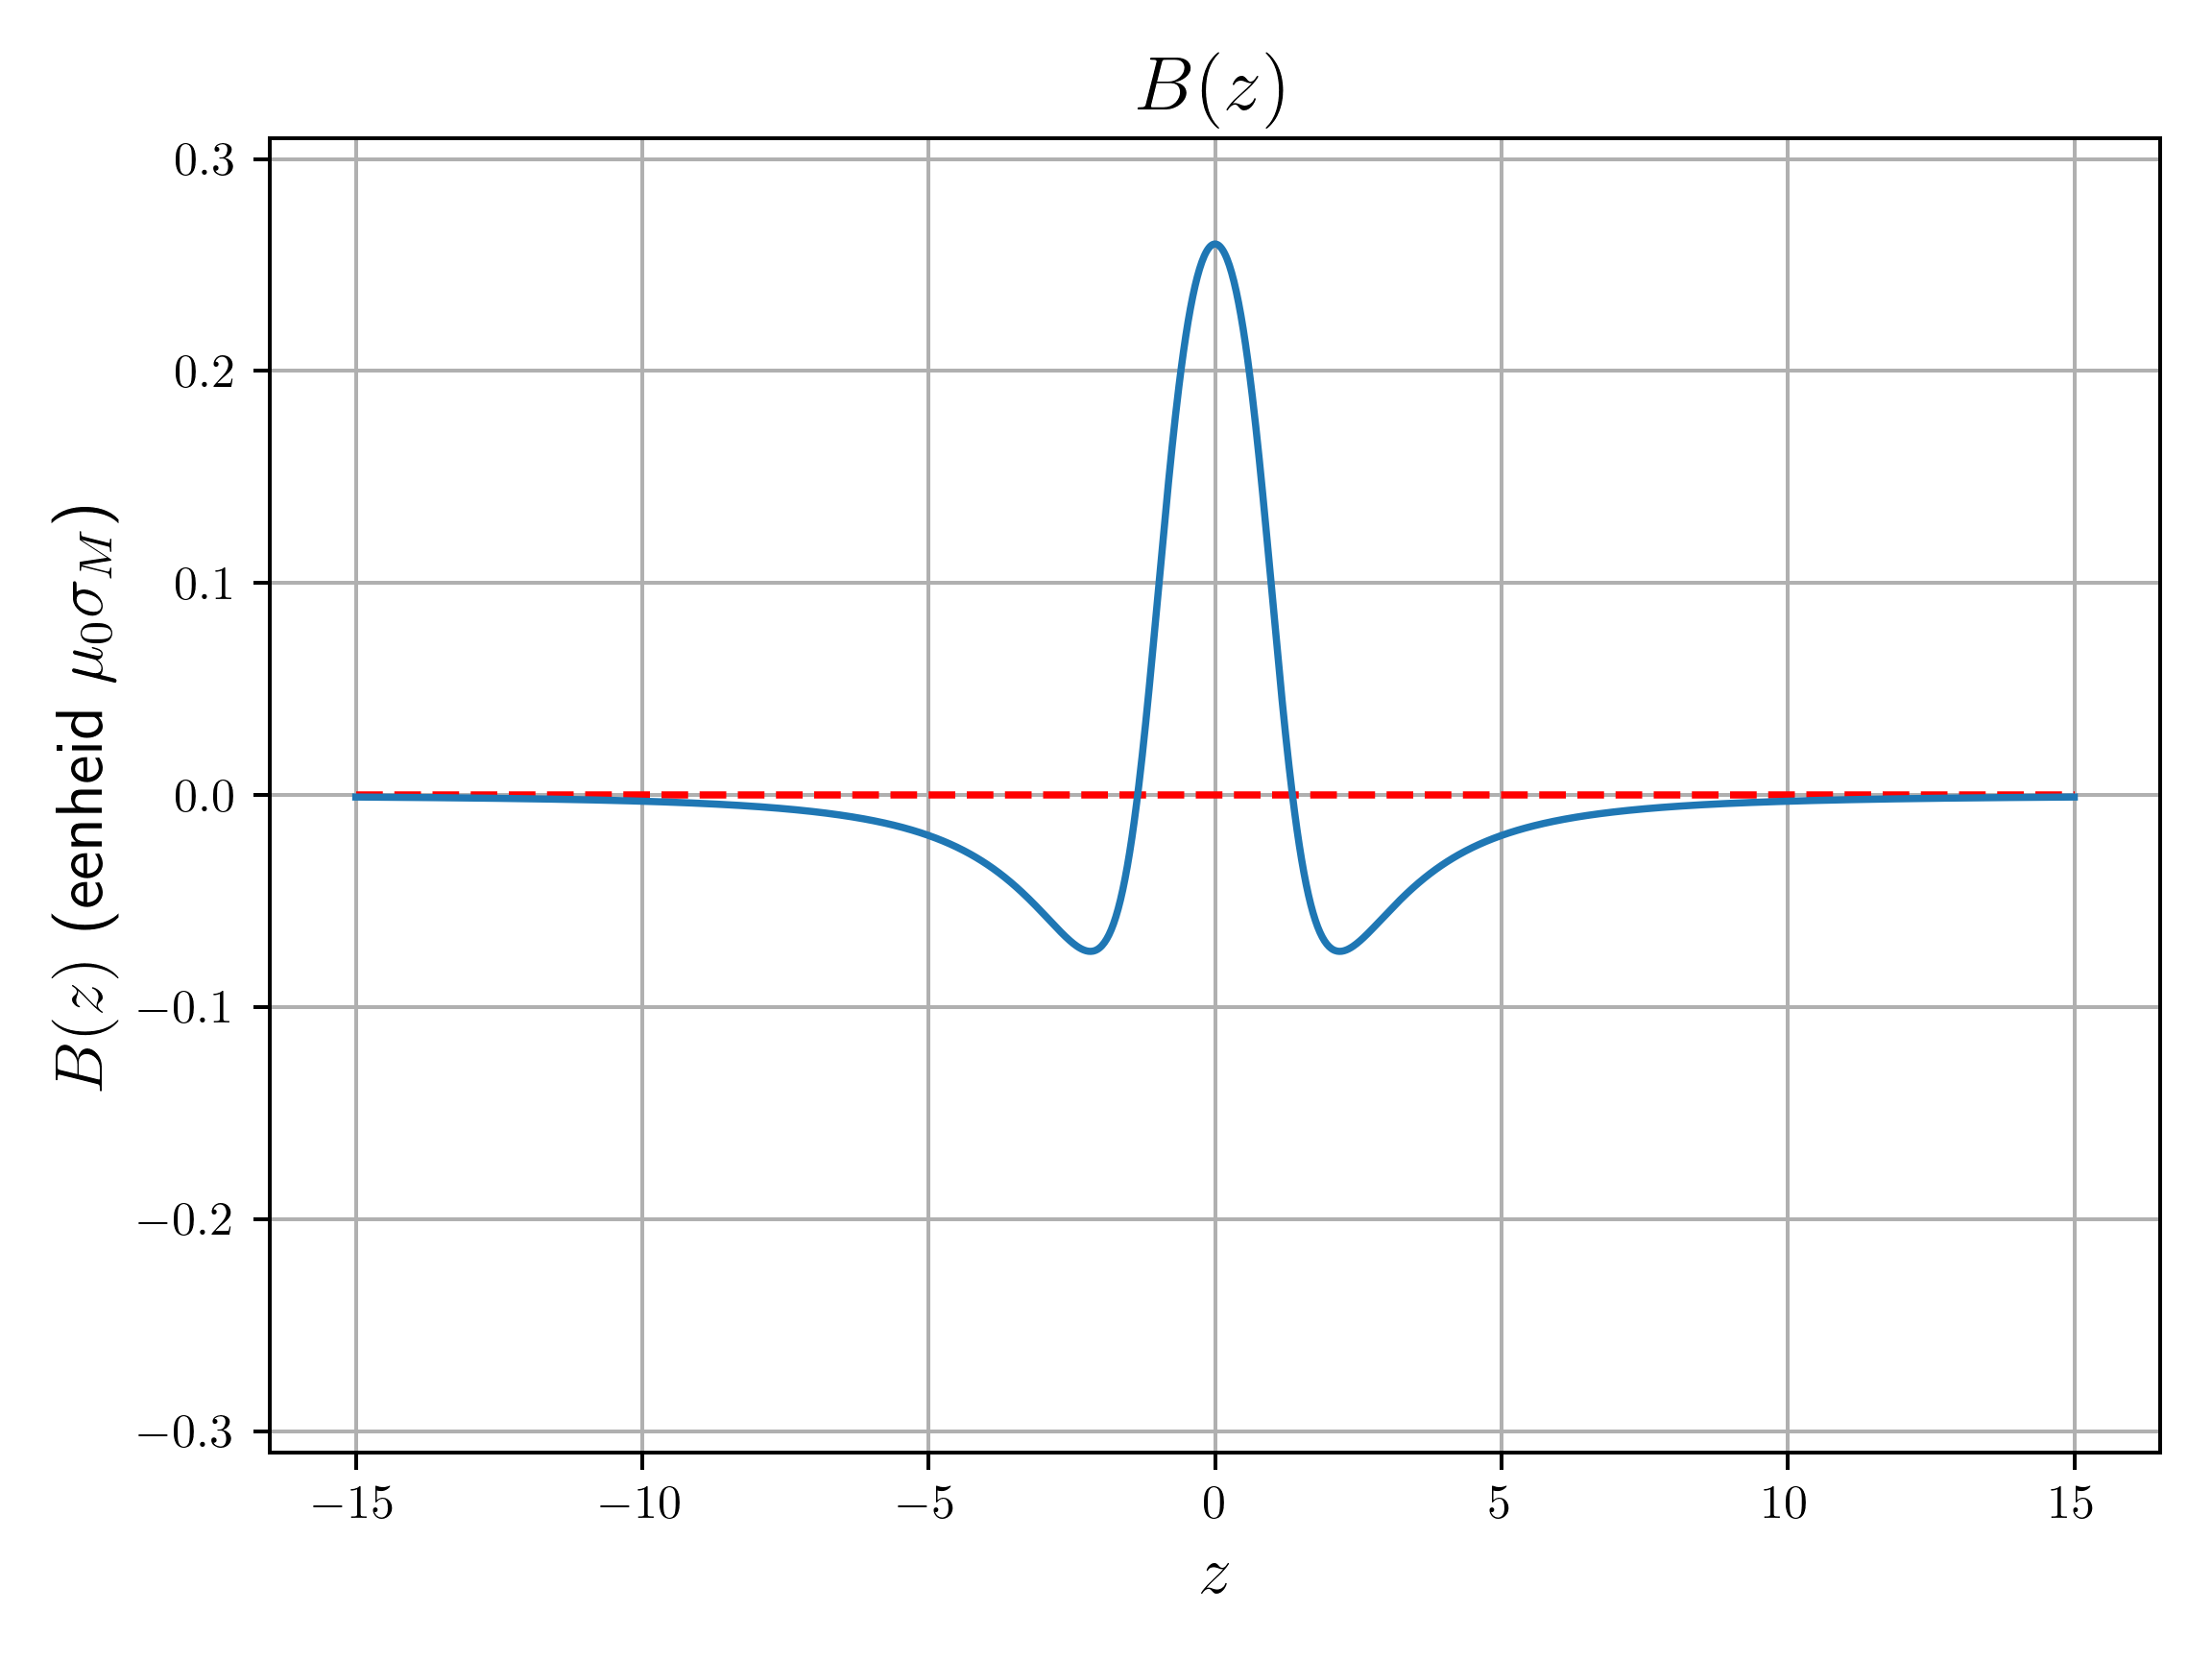
\includegraphics[width=0.6\linewidth]{Images/B_field_2_annula.png}
    \caption{Plot van $B$ volgens vergelijking \ref{eq:2_annula} voor parameters $R_1=1$, $R_2=2$, en $d=2$. Het veld is nu symmetrisch rond het midden van de lens en maximaal in het midden van de lens, zoals men zou verwachten.}
    \label{fig:B_field_2_annula}
\end{figure}
We verkrijgen op deze manier een sterk gepiekt magnetisch veld in het midden van de lens. Dit is exact wat we willen om een dunne lens met een bruikbare focale lengte te maken. Later zullen we onderzoeken hoe de geometrie van de ringoppervlakken het magnetisch veld verandert, en hoe dit de lenseigenschappen beïnvloedt.\\

Een belangrijke opmerking bij deze afschatting is dat deze in principe enkel geldt in het gebied $-\frac{d}{2}<z<\frac{d}{2}$. De ringvormige ladingsoppervlakken zijn aan de buitenkanten immers begrensd door de poolschoenen, die een veel grotere permeabiliteit dan vacuüm hebben. In het ideale geval is het magnetisch veld geconcentreerd in de poolschoenen zonder dat het weglekt, en geldt er voor $z>\left|\frac{d}{2}\right|$ dat $B(z)=0$. Op bovenstaande figuur is echter te zien dat de velden buiten de lens heel wat kleiner zijn dan de velden in het centrum van de lens, en aangezien we in de paraxiale bewegingsvergelijking werken met $B^2$ zullen deze randvelden zeer weinig invloed hebben wanneer we de vergelijking numeriek zullen oplossen.\\

Om later de aberratiecoëfficienten te berekenen is het ook nuttig om de analytische afgeleiden van het veld te berekenen. Deze werden geëvalueerd met Wolfram Mathematica en worden hieronder gegeven:
\begin{equation}
    B_{ring}(z)'= \frac{\mu_0\sigma_Mz}{2} \left(\frac{z}{\left(R_2^2+z^2\right){}^{3/2}}-\frac{z}{\left(R_1^2+z^2\right){}^{3/2}}\right)+\frac{1}{\sqrt{R_1^2+z^2}}-\frac{1}{\sqrt{R_2^2+z^2}}
\end{equation}

\begin{equation}
    B(z)'= B_{ring}\left(z+\frac{d}{2}\right)' - B_{ring}\left(z-\frac{d}{2}\right)'
\end{equation}

\begin{equation}
\begin{split}
    B_{ring}(z)''= & \frac{\mu_0\sigma_Mz}{2} \left(\frac{3 z^2}{\left(R_1^2+z^2\right){}^{5/2}}-\frac{3 z^2}{\left(R_2^2+z^2\right){}^{5/2}}-\frac{1}{\left(R_1^2+z^2\right){}^{3/2}}+\frac{1}{\left(R_2^2+z^2\right){}^{3/2}}\right)\\
    &+2 \left(\frac{z}{\left(R_2^2+z^2\right){}^{3/2}}-\frac{z}{\left(R_1^2+z^2\right){}^{3/2}}\right)
\end{split}
\end{equation}

\begin{equation}
   B(z)''= B_{ring}\left(z+\frac{d}{2}\right)'' - B_{ring}\left(z-\frac{d}{2}\right)''
\end{equation}

Deze functies worden getoond op Figuur \ref{fig:derivatives2x2}.
\begin{figure}[H]
    \centering

    \begin{subfigure}[b]{0.45\linewidth}
        \centering
        
\includegraphics[width=\linewidth]{Images/B_field_1_annulus_d1.png}
        \caption{Eerste afgeleide van $B_{ring}(z)$.}
        \label{fig:B_field_1_annulus_d1}
    \end{subfigure}
    \hfill
    \begin{subfigure}[b]{0.45\linewidth}
        \centering
        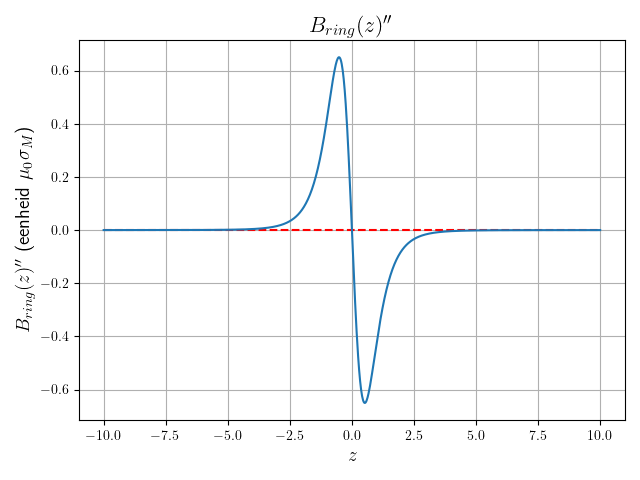
\includegraphics[width=\linewidth]{Images/B_field_1_annulus_d2.png}
        \caption{Tweede afgeleide van $B_{ring}(z)$.}
        \label{fig:B_field_1_annulus_d2}
    \end{subfigure}

    \vspace{0.5cm} 
    \begin{subfigure}[b]{0.45\linewidth}
        \centering
        
\includegraphics[width=\linewidth]{Images/B_field_2_annula_d1.png}
        \caption{Eerste afgeleide van $B(z)$.}
        \label{fig:B_field_2_annula_d1}
    \end{subfigure}
    \hfill
    \begin{subfigure}[b]{0.45\linewidth}
        \centering
        
\includegraphics[width=\linewidth]{Images/B_field_2_annula_d2.png}
        \caption{Tweede afgeleide van $B(z)$.}
        \label{fig:B_field_2_annula_d2}
    \end{subfigure}

    \caption{Plots van de analytische afgeleiden van de magnetische velden voor 1 annulus en 2 annula met $R_1=1$, $R_2=2$, en $d=2$. Deze afgeleiden zullen we later gebruiken om de asymtotische aberratiecoëfficienten van de lens te berekenen.}
    \label{fig:derivatives2x2}
\end{figure}

Onze analytische afschatting kunnen we numeriek controleren met het ionen- en elektronenoptica simulatieprogramma \textit{SIMION}. Dit programma vindt de scalaire magnetische potentiaal door de Laplace-vergelijking voor een ladingsdichtheidverdeling op te lossen. Het programma kan dit door middel van finite-difference methoden; in dit geval werd het veld opgelost met een iteratieve over-relaxatie solver \cite{SIMIONuserguide}. SIMION is bovendien ontworpen om axissymetrische problemen als 2D-problemen op te lossen. Om het numeriek gevonden veld te vergelijken met de analytische uitdrukking, simuleerden we een systeem met twee homogeen geladen ringoppervlakken met $R_1=2\mathrm{mm}$, $R_2=3\mathrm{mm}$ en $d=4\mathrm{mm}$. De magnetische potentiaal werd berekend in een cilindrisch volume met een lengte van $6\mathrm{cm}$ en een straal van $10\mathrm{mm}$, met Dirichlet randvoorwaarden ($\phi=0$ op de rand\footnote{In werkelijkheid willen we $\phi=0$ op oneindig, maar we kunnen geen oneindig groot volume simuleren.}). De potentiaal op de symmetrie-as werd geëxporteerd, en het magnetisch $B(z)=\frac{\delta \phi}{\delta z}$ veld werd numeriek in Python berekend. Op Figuur \ref{fig:B_field_SIMION} worden de analytische en numerieke velden vergeleken. Beide velden werden herschaald zodat $B_{max}=1$ aangezien we nog geen uitdrukking hebben voor $\sigma_M$. We zien een zeer goede overeenkomst, wat aangeeft dat onze analytische uitdrukking correct is.
\begin{figure}[H]
    \centering
    
\includegraphics[width=0.6\linewidth]{Images/B_field_SIMION.png}
    \caption{Vergelijking tussen analytische uitdrukking en numeriek gesimuleerd veld voor $R_1=2\mathrm{mm}$, $R_2=3\mathrm{mm}$ en $d=4\mathrm{mm}$. We zien dat de velden zeer goed overeenkomen.}
    \label{fig:B_field_SIMION}
\end{figure}

\begin{tcolorbox}[colback=blue!10!white,colframe=blue!75!black,title=Realisatie objectief 2]
    Het magnetisch veld op de symmetrie-as werd met een analytische uitdrukking benaderd door de oppervlakken van de poolschoenen te modelleren als twee oppervlakken met een homogene, tegengestelde polladingsdichtheid. Het gebruiken van een analytische uitdrukking laat toe om ook de analytische afgeleiden te berekenen welke gebruikt kunnen worden om aberratiecoëfficienten te schatten. Een vergelijking van de analytische uitdrukking met een numerieke oplossing m.b.v. SIMION van de Laplace-vergelijking geeft een vrijwel perfecte overeenkomst.
\end{tcolorbox}

\section{Magnetische reluctantie van het circuit}
Nu we een benaderende analytische uitdrukking hebben gevonden voor het magnetisch veld voor ons lensontwerp, moeten we nadenken over welke waarde we moeten gebruiken voor de oppervlaktepoolladingsdichtheden $\sigma_M$. \\

De eerste factor waar we rekening mee moeten houden is de reluctantie van het circuit. De Nd-magneet heeft een remanent magneetveld $B_r$, dit is het magnetisch veld dat in de magneet overblijft wanneer we geen uitwendige magnetische velden aanleggen. Wanneer we de magneet in een magnetisch circuit met een luchtspleet gebruiken, zorgen de oppervlakteladingen aan de luchtspleet voor een demagnetiserend veld in de poolschoenen en de magneet dat het remanent veld tegenwerkt. Hierdoor is het werkelijke veld in de magneet $B_m$ kleiner dan het remanent veld $B_r$.\\

Een elegante manier om dit effect wiskundig te beschrijven, is om de analogie te maken met elektrische weerstand en een magnetisch circuit te tekenen dat equivalent is met de geometrie van de lens. We maken eerst een magnetisch circuit equivalent\footnote{De figuur toont dus geen doorsnede van de lens, maar equivalent circuit dat niet meer axissymetrisch is.} aan de cilindrisch symmetrische lens, zoals wordt getoond op Figuur \ref{fig:magnetic_circuit_a}. We krijgen door de oppervlakteladingen een demagnetiserend veld, getoond op Figuur \ref{fig:fields_comparison_b}. Vervolgens tekenen we een symbolisch schema van dit circuit, getoond op Figuur \ref{fig:magnetic_circuit_c}. De magneet is dan een bron van magnetomotorische kracht $\mathcal{F}$. Zowel de magneet, de twee poolschoenen als de luchtspleet zorgen voor een reluctantie $\mathcal{R}$ in het circuit. De magnetische flux doorheen het circuit wordt dan gegeven door:
\begin{equation}\label{eq:flux_mmf_reluctance}
    \Phi = \frac{\mathcal{F}}{\mathcal{R}_{tot}}
\end{equation}

\begin{figure}[H]
    \centering
    \begin{subfigure}[b]{0.35\linewidth}
        \centering
        
\includegraphics[width=\linewidth]{Images/magnetic_circuit.png}
        \caption{}
        \label{fig:magnetic_circuit_a}
    \end{subfigure}
    \hfill
    \begin{subfigure}[b]{0.25\linewidth}
        \centering
        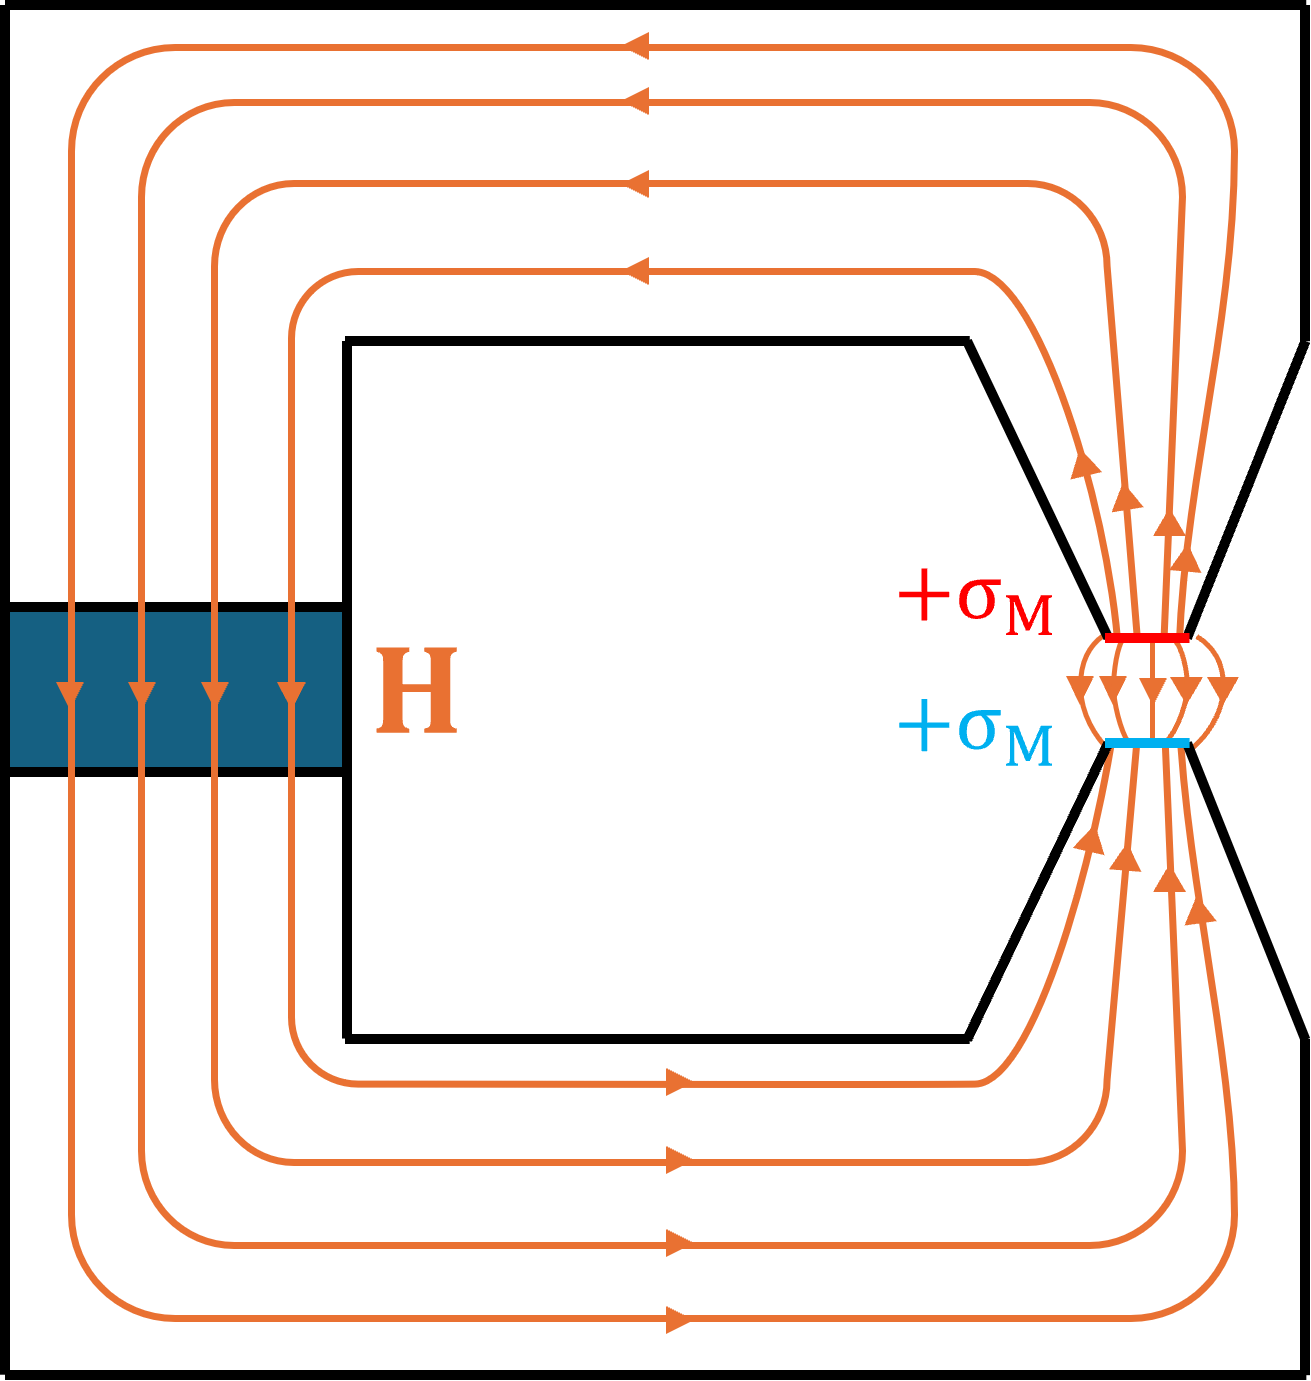
\includegraphics[width=\linewidth]{Images/magnetic_circuit_Hd.png}
        \caption{}
        \label{fig:magnetic_circuit_b}
    \end{subfigure}
    \hfill
    \begin{subfigure}[b]{0.3\linewidth}
        \centering
        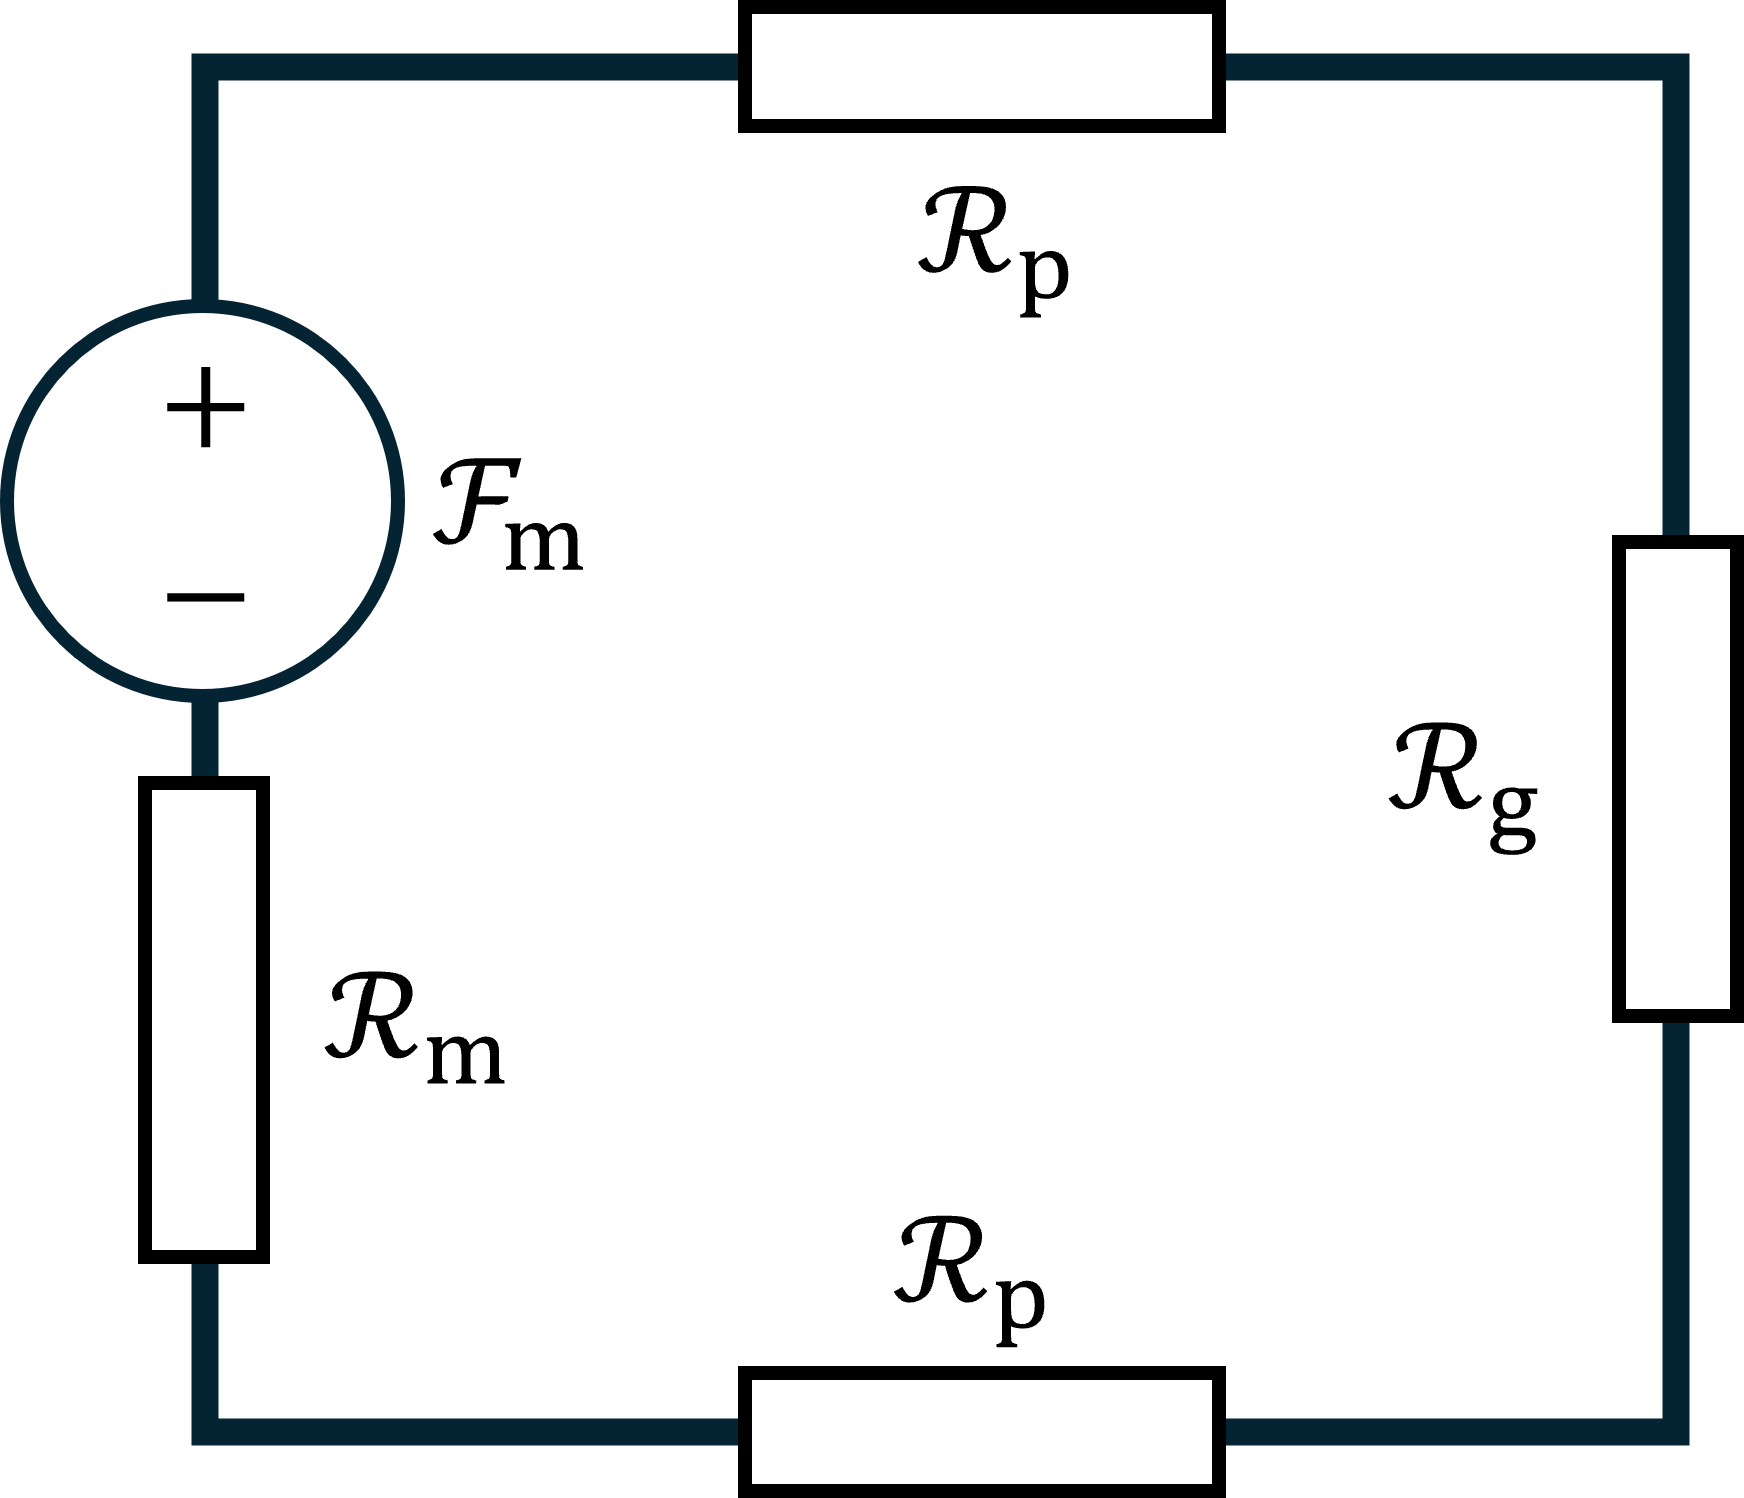
\includegraphics[width=\linewidth]{Images/magnetic_circuit_symbolic.png}
        \caption{}
        \label{fig:magnetic_circuit_c}
    \end{subfigure}
    \caption{Illustratie van het magnetisch circuit equivalent aan dat van de lens. De luchtspleet veroorzaakt demagnetiserend veld dat ervoor zorgt dat het oppervlakteveld $B_m$ van de magneet kleiner wordt dan haar remanent veld $B_r$. Dit kunnen we wiskundig beschrijven door de analogie te maken met elektrische circuits, waarbij de magneet een bron van magnetomotorische kracht, en de luchtspleet een reluctantie voorstellen.}
    \label{fig:magnetic_circuit}
\end{figure}

%% Old derivation
% \color{red}
% De totale reluctantie van het circuit kan berekend worden uit\footnote{Hierbij benaderen we de permeabiliteit van lucht $\mu_{lucht}\approx\mu_0$.}:
% \begin{align}
%     & \mathcal{R}_{tot}= \int_\Gamma \frac{dl}{\mu(l)A(l)} = \mathcal{R}_{m} + 2\mathcal{R}_{p} + \mathcal{R}_{g}\\
%     &= \int_{magneet}\frac{dl}{\mu_{m}A(l)} + 2\int_{poolschoen}\frac{dl}{\mu_{p}A(l)} + \int_{luchtspleet}\frac{dl}{\mu_{0}A(l)}
% \end{align}
% De permeabiliteit van de poolschoenen $\mu_p$ is heel groot, dus is $\mathcal{R}_{p}\approx 0$ en verwaarloosbaar. We kunnen de reluctantie van de magneet en de luchtspleet nu expliciet uitschrijven in functie van de lensparameters, met $A_m = \pi\left(R_{2, m}^2-R_{1, m}^2\right)$ de oppervlakte van de ringmagneet en $A_g = \pi\left(R_{2}^2-R_{1}^2\right)$ de oppervlakte van de poolschoenen aan de luchtspleet. Hierbij verwaarlozen we het naar buiten buigen van de veldlijnen, wat $A_g$ iets groter zou maken. Dit effect is echter klein in verhouding met de oppervlakte van de poolschoenen. De totale reluctantie wordt dan:
% \begin{equation}
%     \mathcal{R}_{tot}=\frac{d_m}{\mu_m A_m}+\frac{d_g}{\mu_0 A_g}
% \end{equation}
% Waarbij $d_m$ en $d_g$ respecievelijk de dikte van de magneet en van de luchtspleet voorstellen. De magnetomotorische kracht van de magneet wordt gegeven door:
% \begin{equation}
%     \mathcal{F}_m = H_c d_m = \frac{B_r d_m}{\mu_m }
% \end{equation}
% Hierbij geldt er dat $B_r = \mu_m H_c$ zolang de poolschoenen niet gesatureerd raken en de $B-H$ curve lineair blijft. Nu kunnen we de totale flux doorheen het circuit berekenen:
% \begin{equation}
%     \Phi = B_r\frac{d_m}{\mu_m  \left(\frac{d_m}{\mu_m A_m}+\frac{d_g}{\mu_0 A_g}\right)}=B_r\frac{A_m}{\left(1+\frac{\mu_m d_g A_m}{\mu_0 d_m A_g}\right)}
% \end{equation}
% De werkelijke magnetische fluxdichtheid $B_m$ in de magneet vinden we door de flux te delen door het oppervlak $A_m$:
% \begin{equation}
%     B_m = B_r\frac{1}{\left(1+\frac{\mu_m d_g A_m}{\mu_0 d_m A_g}\right)}
% \end{equation}
% De correctieterm geeft dus aan welke fractie van het magnetisch veld er overblijft wanneer we het demagnetiserend veld $H_d$ in rekening nemen. Het is meer gebruikelijk om dit uit te drukken als de interne permeantiecoëfficiënt $P_{ci}=\frac{B_m}{\mu_m H_d}$. Deze kunnen in dit specifiek geval uitrekenen:
% \begin{equation}
%     \frac{B_m}{B_r}=\frac{B_r-\mu_m H_d}{B_r} = \frac{1}{\left(1+\frac{\mu_m d_g A_m}{\mu_0 d_m A_g}\right)}\Leftrightarrow P_{ci} = \frac{d_m A_g}{d_g A_m}+\frac{\mu_m}{\mu_0}
% \end{equation}
% \color{black}

Ten eerste weten we dat dezelfde flux doorheen het oppervlak van de magneet en het oppervlak van de luchtspleet stroomt, aangezien $\nabla \cdot \mathbf{B}=0$. Er geldt dus:
\begin{equation}\label{eq:B_m_B_g}
    B_m A_m = B_g A_g
\end{equation}
De totale reluctantie van het circuit kan berekend worden door de reluctanties in serie op te tellen $\mathcal{R}_{tot}=\mathcal{R}_{m}+2\mathcal{R}_{p}+\mathcal{R}_{g}$. Door de grote permeabiliteit van de poolschoenen $\mu_p$ is $\mathcal{R}_{p}$ verwaarloosbaar, dus $\mathcal{R}_{tot}=\mathcal{R}_{m}+\mathcal{R}_{g}$. We houden dus enkel rekening met de reluctanties van de magneet en de luchtspleet. Uit de wet van Ampère in integraalvorm vinden we:
\begin{equation}\label{eq:H_m_H_g}
    \int_\Gamma \mathbf{H}\cdot d\mathbf{l} \approx H_g d_g - H_m d_m = I_{int}=0 \Leftrightarrow H_m = \frac{d_g}{d_m}H_g
\end{equation}
Waarbij $d_m$ en $d_g$ respecievelijk de dikte van de magneet en van de luchtspleet voorstellen. Nu weten we dat er in de luchtspleet geldt dat $H_g = \frac{B_g}{\mu_0}$, wat we kunnen invullen in \ref{eq:B_m_B_g}:
\begin{equation}
    H_g = \frac{B_m A_g}{\mu_0 A_g}
\end{equation}
Door dit dan weer in te vullen in \ref{eq:H_m_H_g} vinden we de relatie:
\begin{equation}
    H_m = \frac{B_m A_g d_g}{\mu_0 A_g d_m} \Leftrightarrow \frac{B_m}{\mu_0 H_m} = \frac{A_g d_m}{A_g d_g} = P_c
\end{equation}
Deze coëfficiënt $P_c$ wordt de \textit{permeantiecoëccifient} genoemd en drukt de verhouding uit tussen de overgebleven magnetische fluxdichtheid en het demagnetiserend veld in de magneet \cite{mmpa_permanent_magnet_guidelines}. Voor onze doeleinden is het gemakkelijker om te werken met de intrinsieke permeantiecoëccifient $P_{ci}$, welke het verband uitdrukt tussen het remanent veld $B_r$ en het demagnetiserend veld $H_d$.
\begin{equation}
    P_{ci}=\frac{B_r}{\mu_0 H_m}=\frac{B_m+\mu_0 H_m}{\mu_0 H_m}=1+\frac{B_m}{\mu_0 H_m}=1+P_c = 1+\frac{A_g d_m}{A_g d_g}. 
\end{equation}

Het demagnetiserend veld zal enerzijds het remanent veld van de magneet tegenwerken, maar zal anderzijds ook het remanent veld zelf doen verkleinen. Hiervoor moeten we kijken naar de $\mathrm{BH}$-curve van de magneet die we gebruiken. Figuur \ref{fig:BH_curve_NdFeB} toont de $\mathrm{BH}$-curve van graad N35 NdFeB voor verschillende temperaturen. Op de figuur staan zowel de normale ($B_m(H_d)$) als de intrinsieke ($B_r(H_d)$) $\mathrm{BH}$-curve voor 6 verschillende temperaturen. In ons geval zijn we geïnteresseerd in de intrinsieke $\mathrm{BH}$-curve bij kamertemperatuur, welke wordt gegeven door de gekromde blauwe lijn. We willen het zogenaamde \textit{werkingspunt} van de magneet bepalen, dit is het $(B_r, H_d)$ punt op de curve waarop het systeem zich bevindt. Dit doen we door het snijpunt te vinden tussen de interne $\mathrm{BH}$-curve en de rechte gegeven door $P_{ci} \mu_0 H_m=B_r$, de \textit{load line}. Een voorbeeld wordt getoond op Figuur \ref{fig:operating_point} waarbij $P_{ci}=1.5$.\\

\begin{figure}[H]
    \centering
    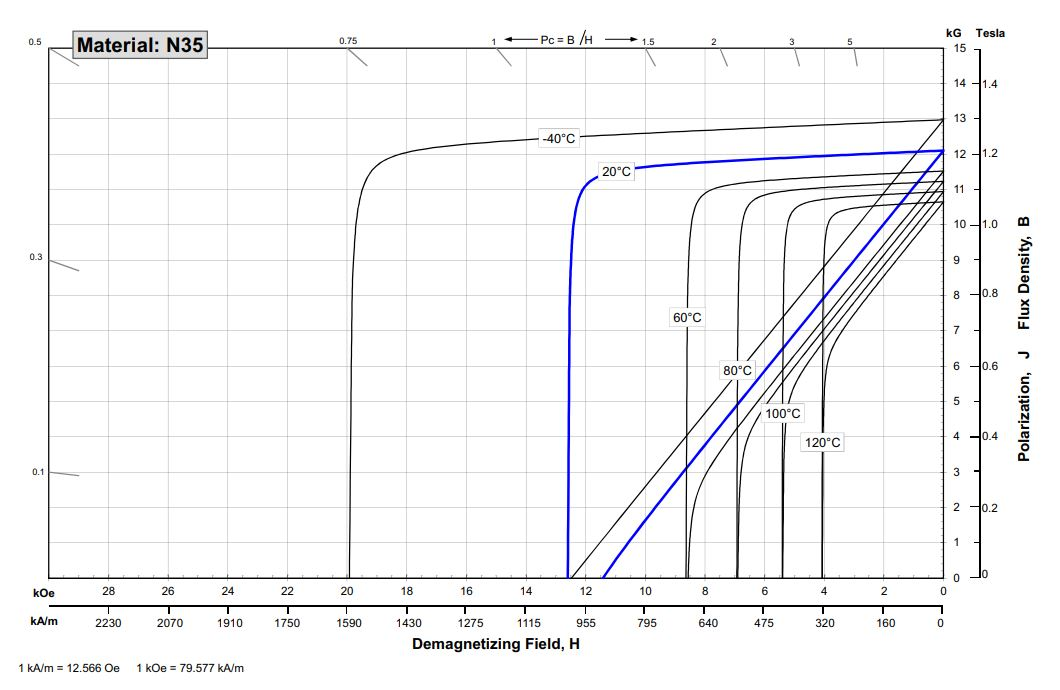
\includegraphics[width=0.6\linewidth]{Images/BH_curve_NdFeB.JPG}
    \caption{$\mathrm{BH}$-curve van graad N35 NdFeB voor verschillende temperaturen. Het aanleggen van een demagnetiserend veld doet de intrinsieke sterkte van de magneet licht verkleinen. Bij een zeer groot (extern) demagnetiserend veld passeren we de elleboog van de $\mathrm{BH}$-curve en demagnetiseert de magneet, of wordt deze zelfs omgepoold. \cite{arnold_ndfeb_2019}}
    \label{fig:BH_curve_NdFeB}
\end{figure}

\begin{figure}[H]
    \centering
    
\includegraphics[width=0.6\linewidth]{Images/operating_point_15.png}
    \caption{Het werkingspunt van de magneet kunnen we vinden door het snijpunt te bepalen van de $\mathrm{BH}$-curve en de load line, waarvan de richtingscoëfficiënt afhant van de intrinsieke permeantiecoëccifient $P_c$. Als het werkingspunt niet voorbij de elleboog van de curve ligt, dan zal de magneet niet demagnetiseren.}
    \label{fig:operating_point}
\end{figure}

Een we het veld gegenereerd door de magneet $B_m=B_r-\mu_0 H_d$ hebben gevongen, kunnen we het magnetisch veld aan het oppervlak grenzend aan de luchtspleet kunnen berekenen door rekening te houden met de oppervlaktes van de poolschoenen $A_g$:
\begin{equation}\label{eq:Br_yoke}
    B_g = \frac{B_m A_m}{A_g}
\end{equation}
Dit kunnen we nu gebruiken om de juiste waarde voor $\sigma_M$ te vinden. Voor een oneindige homogeen geladen vlakke plaat zou er gelden dat $H = \sigma_m$ en dus dat $B = \mu_0 \sigma_M$. In ons geval geldt er dus dat:

\begin{equation}\label{eq:charge_density}
    \sigma_M = \frac{B_m A_m}{A_g \mu_0}
\end{equation}

De volledige analytische uitdrukking van het magnetisch veld op de optische as van de lens verkrijgen we door de ladingsdichtheid in te vullen in vergelijking \ref{eq:2_annula} en wordt dus gegeven door de volgende vergelijking:\small
\begin{equation}\label{eq:analytical_B_field_final}
    B(z) = \frac{B_m A_m}{A_g}
    \begin{aligned}[t]
        &\left[ \frac{z+\frac{d_g}{2}}{2}\left(\frac{1}{\sqrt{\left(z+\frac{d_g}{2}\right)^2+R_1^2}}-\frac{1}{\sqrt{\left(z+\frac{d_g}{2}\right)^2+R_2^2}}\right)\right.\\
        &\left.- \frac{z-\frac{d_g}{2}}{2}\left(\frac{1}{\sqrt{\left(z-\frac{d_g}{2}\right)^2+R_1^2}}-\frac{1}{\sqrt{\left(z-\frac{d_g}{2}\right)^2+R_2^2}}\right)\right]
    \end{aligned}
\end{equation}

% \begin{align}\label{eq:analytical_B_field_final_alternative}
%     B(z) & = \frac{B_r}{\left(\frac{A_g}{A_m}+\frac{\mu_m d_g}{\mu_0 d_m}\right)}\sum_{\pm}\pm\frac{\zeta_{\pm}}{2}\left(\frac{1}{\sqrt{\zeta_{\pm}^2+R_1^2}}-\frac{1}{\sqrt{\zeta_{\pm}^2+R_2^2}}\right)\\
%     \zeta_{\pm} & = z \pm \frac{d_g}{2}
% \end{align}
\begin{tcolorbox}[colback=blue!10!white,colframe=blue!75!black,title=Realisatie objectief 3]
    Er wordt rekening gehouden met het demagnetiserend veld, dat de poolladingsdichtheden op de oppervlakken van de poolschoenen doet verkleinen. Een analogie met elektrische circuits laat toe om de permeantiecoëfficiënt van het magnetisch circuit van de lens te berekenen, waarna het werkingspunt op de $\mathrm{BH}$-curve gevonden kan worden. De oppervlaktepoolladingsdichtheid wordt berekend door de benadering te maken dat alle flux in de magneet wordt verdeeld over de oppervlakkes van de poolschoenen.
\end{tcolorbox}

\section{Implementatie in Python}
Om de afhankelijkheid van de lenseigenschappen ($f, z_{Fi}, z_{Pi}$, etc.) van de lensparameters ($R_1, R_2, d_g, B_r$, etc.) te analyseren, hebben we een klasse in Python geschreven. Hiermee kunnen we snel de het magnetisch veld berekenen en plotten voor een bepaalde geometrie van de magneet en de poolschoenen, en vervolgens de paraxiale bewegingsvergelijking voor dit veld oplossen om zo de lenseigenschappen te berekenen. 

\subsection{Paraxiaal magnetisch veld}
Om de afhankelijkheid van het magnetisch veld van de lensparameters te onderzoeken, maken we een functie die ons toelaat om de lensparameters met sliders aan te passen, terwijl het magnetisch veld continu wordt geupdated. In deze functie is ook het remanent veld $B_r$ instelbaar, wat beter gedefiniëerd moet worden aangezien de magneet niet 1 waarde voor $B_r$ heeft (maar een $\mathrm{BH}$-curve). Deze instelling herschaalt de $\mathrm{BH}$-curve zodanig dat het remanent veld voor $H_d=0\frac{\mathrm{A}}{\mathrm{m}}$ gelijk is aan de ingestelde waarde voor $B_r$. Een voorbeeld van een plot wordt getoond op Figuur \ref{fig:Interactive_B_field} voor de parameters $R_1=0.8\mathrm{mm}$, $R_2=3.25\mathrm{mm}$, en $d_g=0.8\mathrm{mm}$.
\begin{figure}[H]
    \centering
    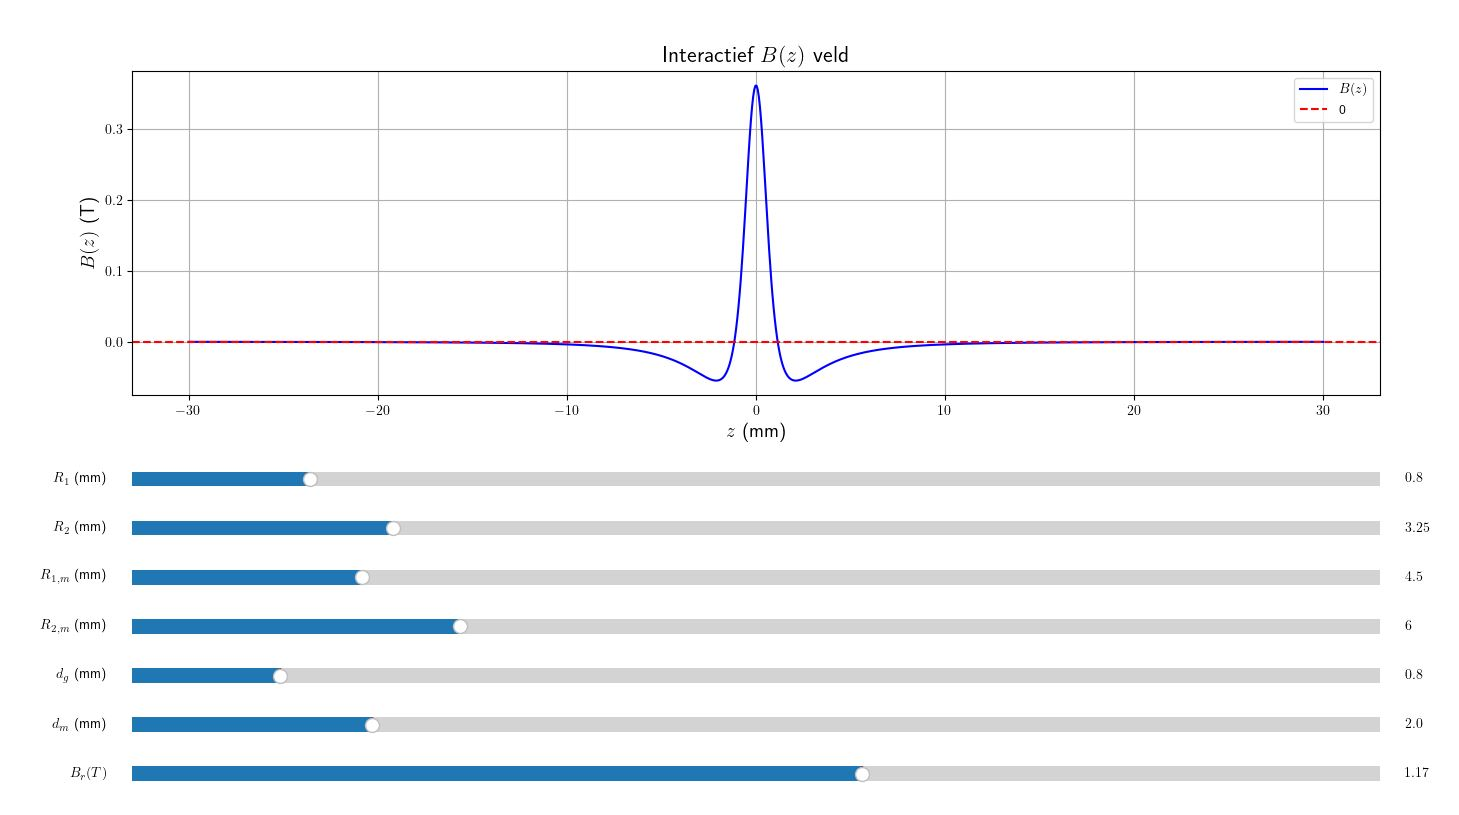
\includegraphics[width=0.6\linewidth]{Images/Interactive_B_field.JPG}
    \caption{Interactieve plot van $B(z)$ in functie van de lensparameters. Deze functie kunnen we gebruiken om de afhankelijkheid van de verschillende parameters te bestuderen, en de lensparameters te optimaliseren om een gewenst magnetisch veld te krijgen. In dit geval gebruiken we de parameters $R_1=0.8\mathrm{mm}$, $R_2=3.25\mathrm{mm}$, en $d_g=0.8\mathrm{mm}$. De $B_r$ instelling zorgt voor een herschaling van de $\mathrm{BH}$-curve.}
    \label{fig:Interactive_B_field}
\end{figure}

\subsection{Paraxiale bewegingsvergelijking}
Met de analytische uitdrukking voor het magnetisch veld kunnen we de paraxiale bewegingsvergelijking oplossen om uiteindelijk de lenseigenschappen van de lens te gaan voorspellen. Ter herinnering, de paraxiale bewegingsvergelijking wordt gegeven door:
\begin{equation}\label{eq:paraxialevgl_rel_H54}
    \frac{d^2r}{dz^2}+\frac{\eta^2B(z)^2}{4V}r=0
\end{equation}
Hoewel de vergelijking er niet al te complex uit ziet, is het helemaal niet triviaal om ze voor eender welk magnetisch veld exact op te lossen. Slechts in enkele gevallen is er een analytische oplossing in gesloten vorm gekend. Een voorbeeld hiervan is \textit{Glaser's bell-shaped field}:
\begin{equation}\label{eq:Glasers_field}
    B(z) = \frac{B_0}{1+\frac{z^2}{a^2}}
\end{equation}
De oplossing van vergelijking \ref{eq:paraxialevgl_rel_H54} kan voor dit veld worden uitgedrukt met goniometrische functies \cite{PWHawkes}. Het magnetisch veld kan ook benaderd worden door een constant veld:
\begin{equation}\label{eq:constant_field}
    B(z) = 
    \begin{cases}
        B_0 & z<\left|\frac{d}{2}\right|\\
        0 & z>\left|\frac{d}{2}\right|\\
    \end{cases}
\end{equation}
In dat geval heleidt vergelijking \ref{eq:paraxialevgl_rel_H54} zich tot een harmonische oscillator in de lens. Echter, beide velden zijn niet fysisch, en slechts benaderingen van werkelijke magnetische velden. Figuur \ref{fig:fields_comparison} geeft een vergelijking tussen deze twee velden en ons afgeschatte veld.
\begin{figure}[H]
    \centering
    \begin{subfigure}[b]{0.3\linewidth}
        \centering
        
\includegraphics[width=\linewidth]{Images/Glasers_B_field.png}
        \caption{}
        \label{fig:fields_comparison_a}
    \end{subfigure}
    \hfill
    \begin{subfigure}[b]{0.3\linewidth}
        \centering
        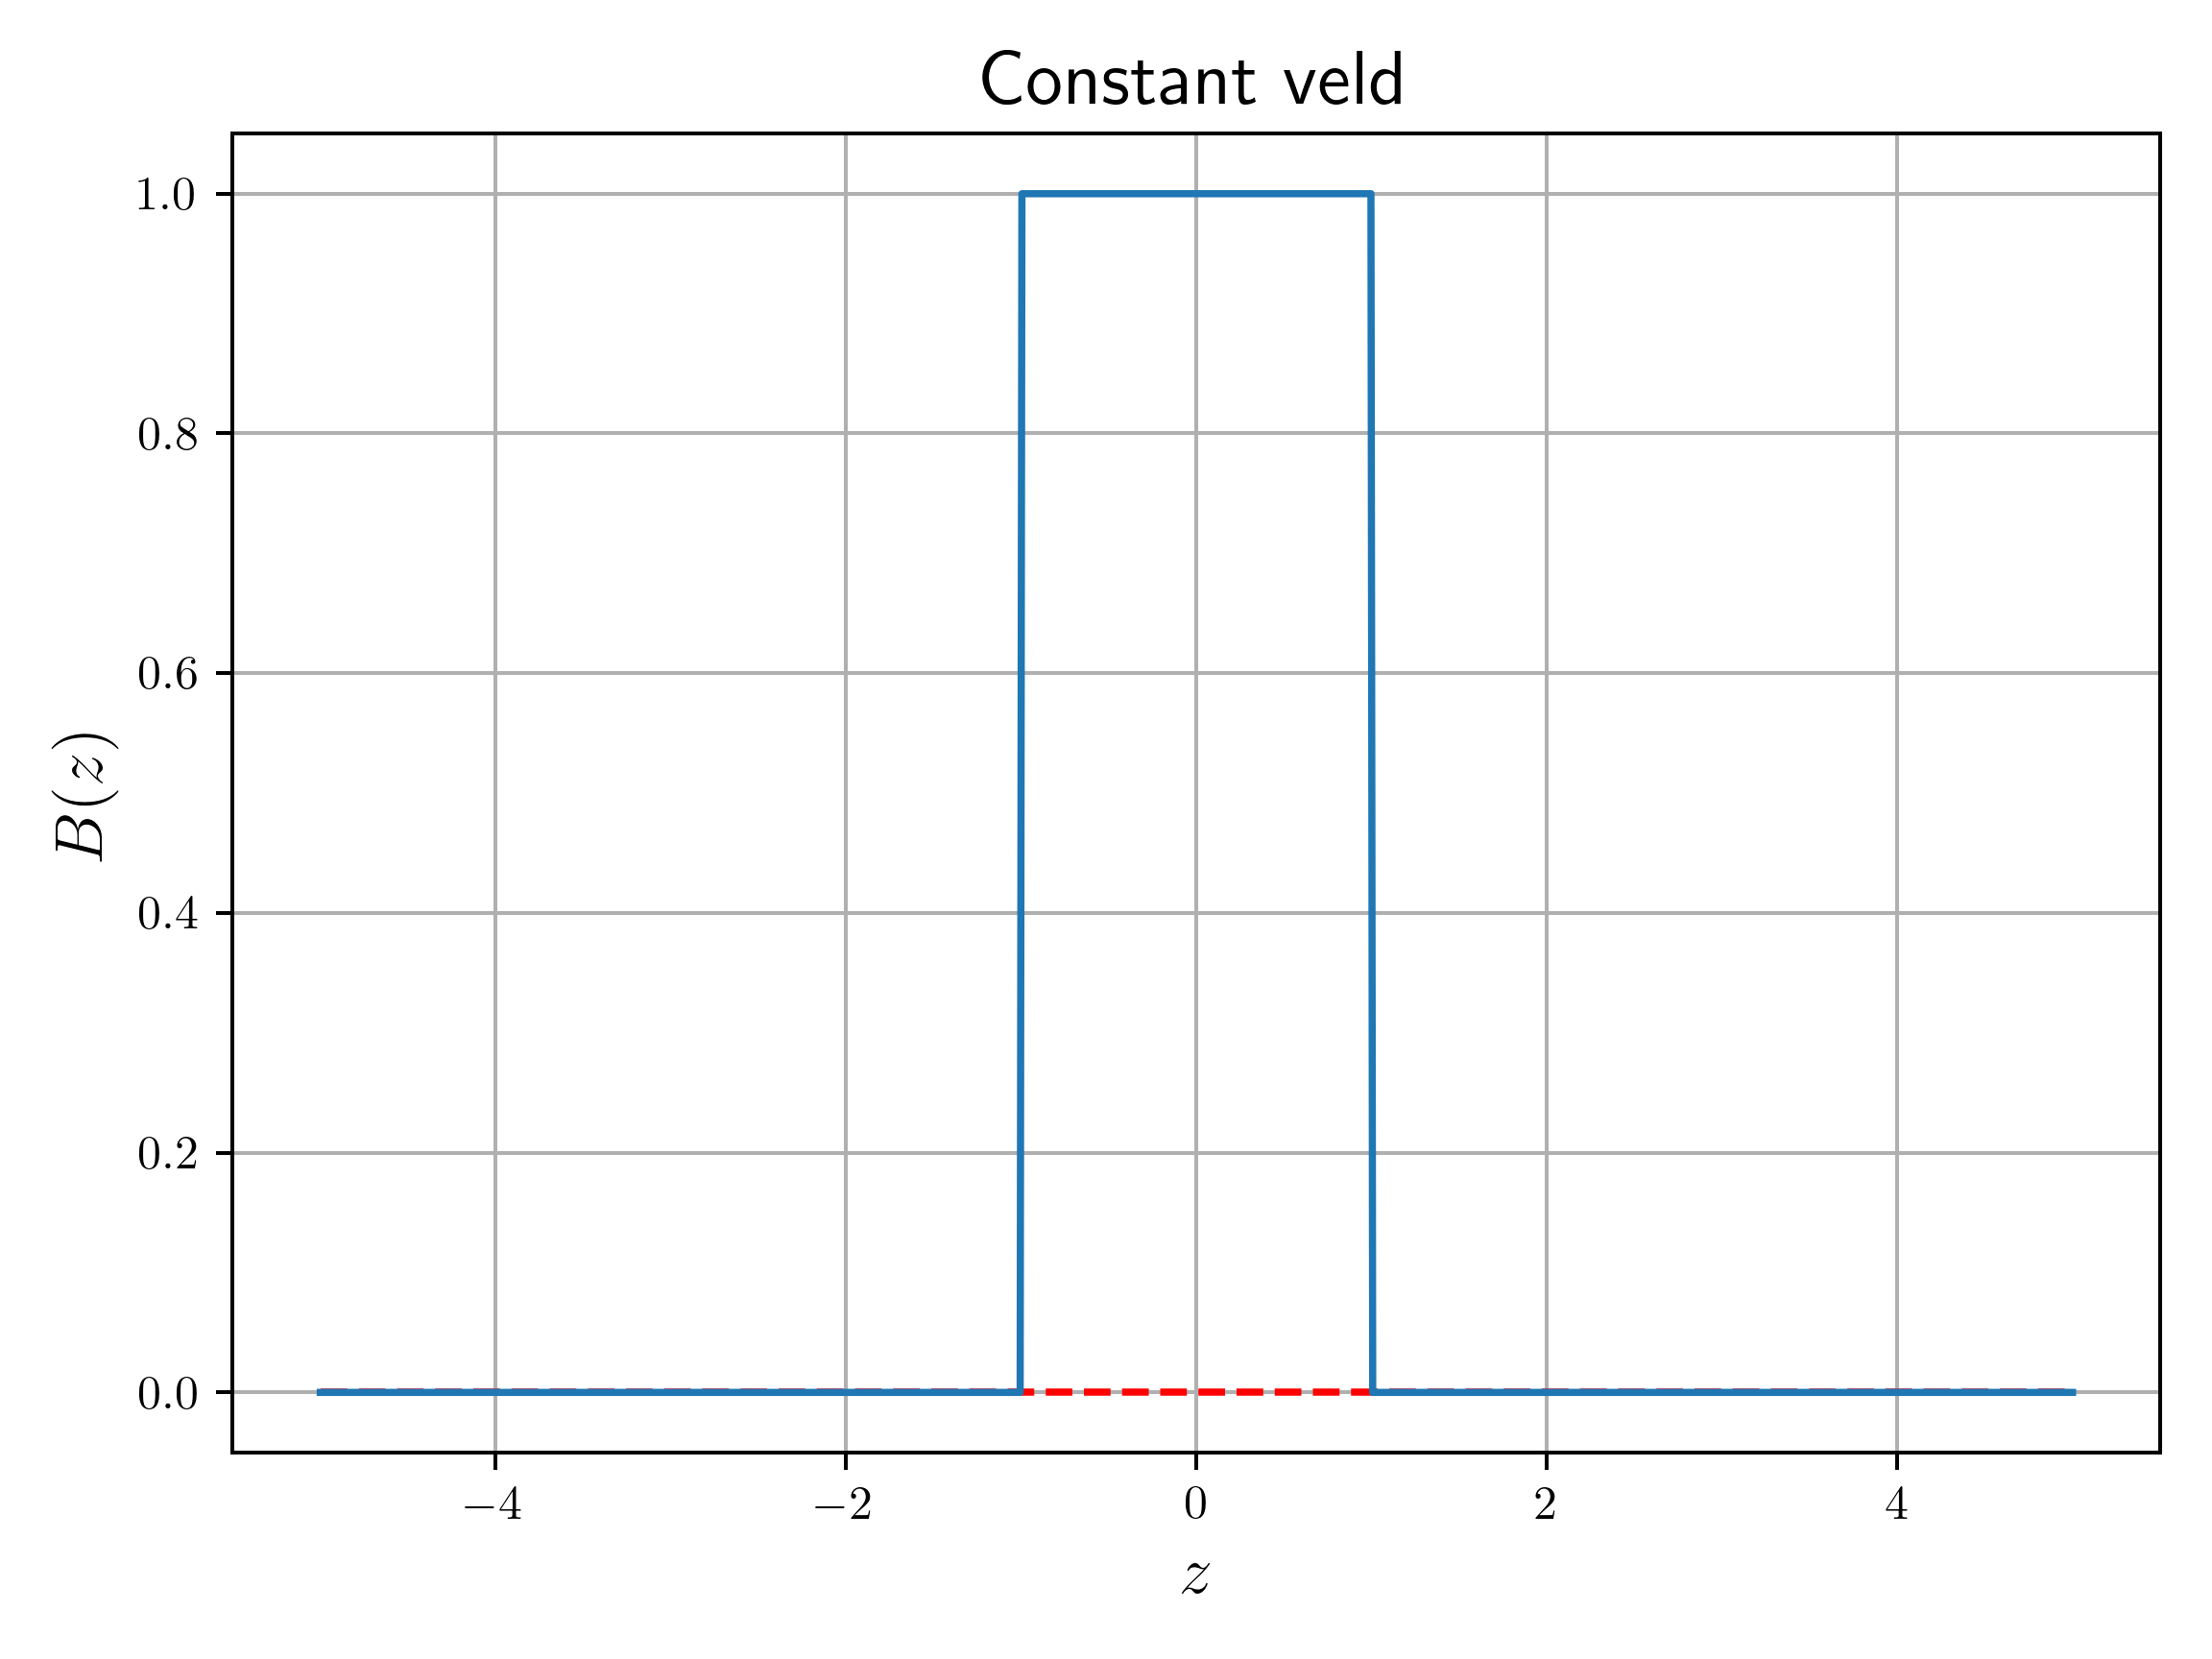
\includegraphics[width=\linewidth]{Images/Constant_B_field.png}
        \caption{}
        \label{fig:fields_comparison_b}
    \end{subfigure}
    \hfill
    \begin{subfigure}[b]{0.3\linewidth}
        \centering
        
\includegraphics[width=\linewidth]{Images/Actual_B_field.png}
        \caption{}
        \label{fig:fields_comparison_c}
    \end{subfigure}
    \caption{Vergelijking tussen twee velden (Glaser's field en constant veld) waarvoor de paraxiale bewegingsvergelijking analytisch oplosbaar is en ons analytisch afgeschat veld. Het Glaser's field is gelijkaardig, maar heeft een bredere piek en valt trager af dan ons afgeschatte veld. Dit geeft een dikkere lens, wat ongewenst is.}
    \label{fig:fields_comparison}
\end{figure}
We zien dat het Glaser's field een goede benadering zou geven, maar de piek in het magnetisch veld is breder het veld vlakt trager af dan het veld van onze lens. Om accurate voorspellingen van onze lens te kunnen maken, kiezen we er daarom voor om de paraxiale beweginsvergelijking numeriek op te lossen en hieruit de lenseigenschappen te bepalen. Dit laat ons ook toe om later Monte Carlo simulaties van experimentele opstellingen uit te voeren, zodat we kunnen inschatten welke opstellingen ons bruikbare resultaten kunnen geven.\\

Om de paraxiale bewegingsvergelijking op te lossen, gebruiken we de solve\_ivp functie van de scipy.integrate bibliotheek. Het objectvlak $z_0$ kunnen we naar wens instellen, en we gebruiken een 8ste orde Runge-Kutta methode (DOP853) om de twee lineair onafhankelijke oplossingen $g$ en $h$ te berekenen. De oplossing $g(z)$, waarvoor geldt dat $g(z_0)=1$ en $g'(z_0)=0$, kunnen we dan gebruiken om de lenseigenschappen te berekenen. Ten eerste kijken we in welk vlak de twee asymtoten van $g(z)$, de object en beeld asymtotische bundels, elkaar snijden. Dit vlak is het achterste/beeld hoofdvlak van de lens $z_{Pi}$. Ten tweede kijken we waar de beeld asymtotische bundel de symmetrie-as van de lens snijdt. Alle parallel bewegende elektronen zullen door dit punt passeren, dus dit is het brandpunt in het focusvlak $z_{Fi}$ van de lens. De brandpuntsafstand kunnen we dan berekenen uit $f=z_{Fi}-z_{Pi}$. Door de symmetrie van het magnetisch veld kunnen we het object beeldvlak en het object focusvlak vinden uit $z_{Po}=-z_{Pi}$ en $z_{Fo}=-z_{Fi}$, Figuur \ref{fig:setup_1} toont een voorbeeld van een numerieke oplossing van $g$. In dit geval vinden we een brandpuntsafstand van $f=15.50\mathrm{mm}$ en bevindt het beeld hoofdvlak zich op $z_{Pi}=-0.33\mathrm{mm}$ van het midden van de lens.\\

Eens we de twee lineair onafhankelijke oplossingen hebben berekend, is het mogelijk om de baan van eender welk elektron af te beelden door een lineaire combinatie van de twee oplossingen te maken. Op deze manier kunnen we stralingsdiagrammen zoals Figuur \ref{fig:setup_2}, waarbij we de lens van de voorgaande figuur hebben gebruikt om een vergroting van $M=5$ te krijgen. We tekenen op de figuur de drie hoofdstralen: de straal die door het midden van de lens gaat, en de straal die door het voorste brandpunt gaat. Deze drie kruisen elkaar in 1 punt achter de lens, waar het beeld gevormd wordt. Merk ook op dat de straal die door het midden van de lens gaat bijna niet wordt afgebogen, zoals men zou verwachten bij een dunne lens in de geometrische optica.

\begin{figure}[H]
    \centering
    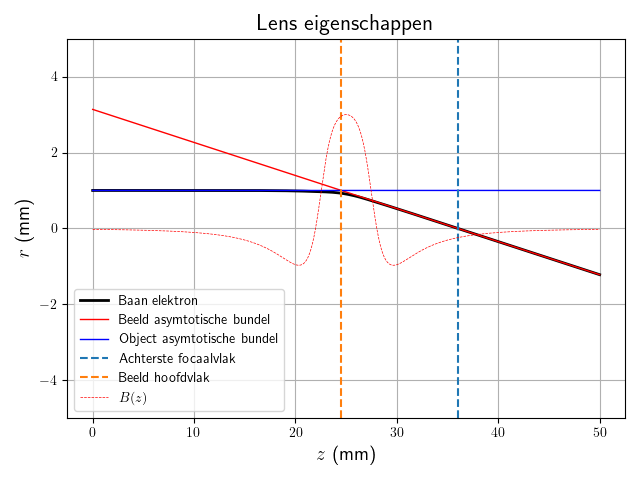
\includegraphics[width=0.6\linewidth]{Images/setup_1.png}
    \caption{Plot van numerieke oplossing van de paraxiale bewegingsvergelijking. De object en beeld asymptotische bundels snijden elkaar in het beeld hoofdvlak, en de beeld asymtotische straal snijdt de symmetrie-as in het achterste focaalvlak van de lens. Deze opstelling heeft de volgende parameters: $R_1=1.5\mathrm{mm},R_2=5\mathrm{mm},d=5\mathrm{mm}, B_g=0.447\mathrm{T},\Phi=30$~keV.}
    \label{fig:setup_1}
\end{figure}

\begin{figure}[H]
    \centering
    
\includegraphics[width=0.6\linewidth]{Images/setup_2.png}
    \caption{Voorbeeld van beeldvorming met een permanente magneetlens. We beschouwen hier de drie hoofdstralen: de straal die door het achterste brandpunt gaat, de straal die door het midden van de lens gaat, en de straal die door het voorste brandpunt gaat. In dit geval krijgen we een vergroting $M=5$.}
    \label{fig:setup_2}
\end{figure}
\subsection{Aberratiecoëfficienten}
Met de analystische afschatting van het veld en de analytische afgeleiden zijn we in staat om de asymtotische aberratiecoëfficiënten in vergelijkingen \ref{eq:distortion} en \ref{eq:chr_ab} van de lens te berekenen. De uitdrukkingen van deze coëfficiënten worden hieronder gertoond \cite{PWHawkes}.
\begin{align}
    D&=\frac{3}{8f}+\frac{\eta^2}{48V}\int_{-\infty}^{+\infty}\left(\frac{4\eta^2}{V}B^4+5B'^2-BB''\right)g^3hdz\\
    C_M&=-\frac{\eta^2}{4V}\int_{-\infty}^{+\infty}B^2ghdz
\end{align}
Merk op dat de oplossinge $g$ en $h$ van vergelijking \ref{eq:gh} optreden. Deze opolssingen worden als dimensieloos beschouwd. Bovendien zijn deze oplossingen afhankelijk van de objectpositie $z_0$, dus zijn ook de aberratiecoëfficienten afhankelijk van de afstand tussen de lens en het object. Deze integralen zijn zeer zelden analytisch oplosbaar, en ook aangezien we geen anaylitische uitdrukkingen voor $g$ en $h$ hebben moeten we deze numeriek oplossen door de Riemann-som met een kleine $\Delta z$ te nemen. 
\color{red} Sferische aberratie ook nog te berekenen \color{black}

\begin{tcolorbox}[colback=blue!10!white,colframe=blue!75!black,title=Realisatie objectief 4]
    Er werd een Python-toolbox geïmplementeerd om de werking van de lens te simuleren waarmee op numerieke wijze de lenseigenschappen voor een bepaalde geometrie bepaald kunnen worden. De paraxiale bewegingsvergelijking wordt opgelost met een $8$ste orde Runge-Kuta methode om  thee linear onafhankelijk oplossingen $g(z)$ en $h(z)$ te vinden, waarna beeldvorming gesimuleerd kan worden door lineaire combinaties van de twee oplossingen te maken. De distortie en chromatische aberratiecoëfficiënten worden geëvalueerd door de integralen van het analytische veld $B(z)$ en haar afgeleiden te benaderen als Riemann-som.
\end{tcolorbox}

\chapter{Optimalisatie en validatie van de lensparameters}\label{ch:optimalisatie}
Eens een simulatietoolbox in Python geïmplmenteerd is, kan deze toegepast worden om de lensparameters te optimaliseren en de lens effectief te realiseren. Hiervoor moeten eerst criteria worden opgesteld waaraan de lens moet voldon om gebruikt te kunnen woden in een elektronenmicroscoop met een versnelspanning van $30$~keV. Vervolgens kunnen de parameters worden afgestemd op deze criteria, waarna de poolschoenen door een CNC-service kunnen worden vervaardigd. Ten slotte kunnen de lenseigenschappen experimenteel worden gekarakteriseerd. De volgende objectieven worden daartoe opgesteld:

\begin{tcolorbox}[colback=red!10!white,colframe=red!75!white,title=Objectief 5]
    Het formuleren concrete criteria waaraan de lensparameters en lenseigenschappen moeten voldoen voor een bruikbare lenswerking.
\end{tcolorbox}

\begin{tcolorbox}[colback=red!10!white,colframe=red!75!white,title=Objectief 6]
    Het gebruiken van de Python-toolbox om de invloed van elke lensparameter afzonderlijk in kaart door variatieplots voor de lenseigenschappen en aberratiecoëfficiënten op te stellen. Op basis van deze analyse kan een optimale set lensparameters geselecteerd worden die maximaal aan de opgestelde criteria voldoet waarmee een 3D-model van de lens met optimale lensparameters in FreeCAD gerealiseerd kan worden.
\end{tcolorbox}

\begin{tcolorbox}[colback=red!10!white,colframe=red!75!white,title=Objectief 7]
    Het karakteriseren van de lens in de elektonenmicroscoop met een versnelspanning van $30$~keV door de focale lengte kwalitatief te berekenen en de aberraties kwantitatief te beschrijven. Dit maakt een vergelijking van de experimentele en gesimuleerde resultaten mogelijk waarmee verschillen kunnen worden geanalyseerd.
\end{tcolorbox}



\section{Lensontwerp}\label{ch:lensontwerp}
Nu we in staat zijn om de banen van elektronen door het magnetisch veld van een lens te simuleren, kunnen de parameters van de lens gaan optimaliseren om een geschikte dunne lens te maken. Hierbij moeten we rekening houden met het volgende:
\begin{enumerate}
    \item De lens moet een dunne lenswerking vertonen, dus moet de positie van het hoofdvlak $z_{Pi}$ zo dicht mogelijk bij het centrum van de lens liggen, m.a.w. $\left|z_{Pi}\right|<0.1\mathrm{mm}$. Dit betekent dat dat $B(z)$ een smalle piek moet vertonen.

    \item We willen een lens die we in de MIRA microscoop kunnen gebruiken. Concreet betekent dit dat we een focale lengte willen die rond de $5-10\mathrm{mm}$ ligt. Hiervoor moet $\sigma_M$ voldoende groot zijn, en moet $R_1$ voldoende klein zijn zodat de ladingen zich niet te ver van de optische as bevinden.
    
    \item We willen dat de berekende aberratiecoëfficiënten $D$ en $C_M$ niet al te groot zijn om vervormde beelden te voorkomen. Typische waarden voor $D$ en $C_M$ zijn respectievelijk $\sim0.5\mathrm{mm}^{-2}$ en $\sim1-3$ \cite{Abbas_2016} \cite{JEOL_Aberrations}. We proberen daarom de coëfficiënten onder deze waarden te houden.

    \item Figuur \ref{fig:operating_point} toonde de $\mathrm{BH}$-curve van graad N35 NdFeB. We willen ten eerste dat het werkingspunt de elleboog van deze curve niet overschrijdt, omdat het remanent veld van de magneet dan snel zou afnemen of zelfs zou omkeren. Echter, de elleboog bevindt zich ongeveer bij $B_r=1.1\mathrm{T}, \mu_0 H_d = 1.2\mathrm{T}$, dus bij $\mu_0 H_d>B_r$. Het is met andere woorden niet mogelijk om de magneet (bij kamertemperatuur) in een circuit te demagnetiseren zonder een extern magnetisch veld aan te leggen.\\

    Echter, het is nog steeds gewenst dat het demagnetiserend veld zo klein mogelijk blijft; een groot demagnetiserend veld zorgt nog steeds voor een instabieler circuit. Een exterm demagnetiserend veld of een hogere temperatuur kunnen de magneet in dat geval makkelijker irreversiebel doen demagnetiseren. In onze berekening van $H_d$ hebben we bovendien een versimpeld en geïdealiseerd systeem beschouwd; dit is slechts een schatting van de exacte waarde. De werkelijke waarde van $H_d$ kan zelfs tot $\sim1.5$ keer groter zijn dan de analytisch geschatte waarde \cite{MagnetFAQ}. Dit betekent dat we de interne permeantiecoëccifient $P_{ci}=\frac{B_r}{\mu_0 H_d}$ liefst zo groot mogelijk houden. Om ongewenste effecten te voorkomen, stellen we voor onszelf een (arbitrair gekozen) ondergrens van $P_{ci}>2.5$ in. Figuur \ref{fig:operating_point_25} toont het werkingspunt bij deze ondergrens.

    \item Een andere belangrijke factor waarmee we rekening moeten houden is de $\mathrm{BH}$-curve van de poolschoenen. We gaan er in vergelijking \ref{eq:Br_yoke} van uit dat alle veldlijnen vanuit de magneet worden uitgespreid over de oppervlaktes van de poolschoenen. In het algemeen is de oppervlakte van de poolschoenen kleiner dan die van de magneet, waardoor de veldlijnen zullen concentreren en de fluxdichtheid toeneemt. Dit betekent dat we moeten oppassen dat de poolschoenen niet gesatureerd raken, want dan zou er magnetisch veld weglekken wat allerlei ongewenste effecten met zich meebrengt. Om een bovengrens voor $B_g$ vast te leggen, moeten we naar de $\mathrm{BH}$-curve van ASI1018 kijken. Deze wordt getoond op Figuur \ref{fig:BH_curve_ASI1018}. Er treedt saturatie op wanneer deze curve afvlakt, dus we willen in het lineair deel van de curve blijven werken. De curve vlakt af bij $\sim1.5\mathrm{T}$, dus willen we dat de maximale fluxdichtheid in onze poolschoenen hieronder blijft. Bij het ontwerp proberen we de parameters zo te kiezen dat $B_g<1.25\mathrm{T}$.

    \item Ten slotte moeten we rekening houden met geometrische beperkingen. De binnenstraal $R_1$ moet groter dan $\sim 0.5\mathrm{mm}$ zijn om te voorkomen dat de elektronen door de gaten van beide poolschoenen kunnen en niet op een oppervlak botsen. De buitenstraal $R_2$ moet uiteraard kleiner zijn dan de binnenstraal van de magneet $R_{1, m}$, maar kiezen we best nog kleiner ($R_2<R_{1, m}-1\mathrm{mm}$) om te voorkomen dat het magnetisch circuit kan kortsluiten doordat de veldlijnen van de magneet naar de oppervlakken van de poolschoenen kunnen overslaan. Bovendien mogen de toleranties van het ontwerp niet te klein worden voor de CNC machines waarmee de poolschoenen gemaakt worden. Bij voorkeur zijn de gekozen afmetingen ook afgeronde getallen, zodat er bv. standaard boorgaten kunnen worden gebruikt bij het produceren van de poolschoenen. Ten slotte kunnen we de afmetingen van de magneet niet vrij kiezen; deze worden niet op maat gemaakt, dus we hebben keuze tussen een beperkt aantal dimensies.
    
\end{enumerate}

\begin{figure}[H]
    \centering
    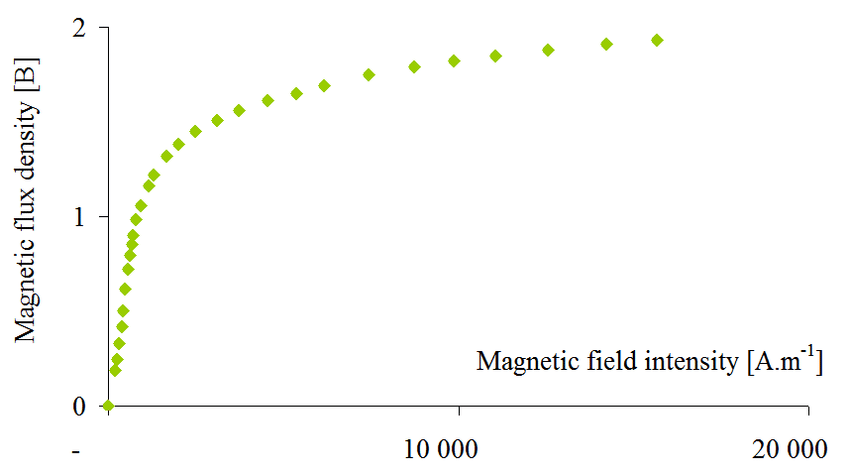
\includegraphics[width=0.75\linewidth]{Images/BH_curve_ASI1018.png}
    \caption{$\mathrm{BH}$-curve van ASI1018. Het is belangrijk dat de curve bij onze waarde voor $B_g$ lineair is, zodat er geen saturatie optreedt en er geen magnetisch veld weglekt. \cite{Buchenau_2014}}
    \label{fig:BH_curve_ASI1018}
\end{figure}

\begin{figure}[H]
    \centering
    
\includegraphics[width=0.75\linewidth]{Images/operating_point_25.png}
    \caption{Het werkingspunt van de magneet bij $P_{ci}=2.5$. Dit is de ondergrens die we voor voor ons ontwerp kiezen om te voorkomen dat er demagnetisatie van de magneet zou optreden. Het werkingspunt kan door een groot aantal onvoorziene factoren dichter dan verwacht bij de elleboog van de curve liggen, dus moeten we ervoor zorgen dat $P_{ci}$ groot genoeg blijft.}
    \label{fig:operating_point_25}
\end{figure}

\begin{tcolorbox}[colback=blue!10!white,colframe=blue!75!black,title=Realisatie objectief 5]
    De permanente magneet lens moet aan de volgende criteria voldoen:
    \begin{table}[H]
    \centering
    \begin{tabular}{@{}cl@{}}
    \toprule
    Lenseigenschap                     & \multicolumn{1}{c}{Waarde}  \\ \midrule
    \multicolumn{1}{|c|}{$f$}        & \multicolumn{1}{c|}{$\sim10\mathrm{mm}$}  \\ \midrule
    \multicolumn{1}{|c|}{$\left|z_{Pi}\right|$}        & \multicolumn{1}{c|}{$<0.1\mathrm{mm}$} \\ \midrule
    \multicolumn{1}{|c|}{$P_{ci}$} & \multicolumn{1}{c|}{$>2.5$}  \\ \midrule
    \multicolumn{1}{|c|}{$B_{max}$} & \multicolumn{1}{c|}{$<1.25\mathrm{T}$}    \\ \midrule
    \multicolumn{1}{|c|}{$D$}        & \multicolumn{1}{c|}{$\leq0.5\mathrm{mm}^{-2}$}    \\ \midrule
    \multicolumn{1}{|c|}{$C_M$}        & \multicolumn{1}{c|}{$\leq3$} \\ \midrule
    \end{tabular}
    \end{table}
    Daarnaast moet de geometrie voldoen aan beperkingen opgelegd door de CNC-toleranties en beschikbare magneetdimensies.
\end{tcolorbox}

\subsection{Simulatie van lenseigenschappen}
Zoals beschreven in hoofdstuk \ref{ch:implementatie}, hebben we in Python een klasse geschreven waarmee we snel de lenseigenschappen van een bepaald lensontwerp kunnen berekenen. Het bepalen van de optimale lensparameters kunnen we hiermee bepalen gewoonweg via trial-and-error, door steeds de lensparameters aan te passen en de lenseigenschappen te berekenen. Het is echter nuttig om de invloed van de verschillende parameters te onderscheiden om ze individueel te kunnen onderzoeken. Hiervoor kiezen we voor een bepaalde lensparameter een boven en ondergrens en berekenen we (voor vaste overige lensparameters) de lenseigenschappen voor een groot aantal punten tussen deze twee grenzen. De resultaten kunnen we dan op een grafiek weergeven om zo efficiënter de lensparameters te optimaliseren. We hebben voor vier verschillende lensparameters ($R_1$, $R_2$, $d_g$, en $B_r$) een functie geïmplementeerd waarmee we dit soort grafieken kunnen plotten. Op deze grafieken plotten we ook de permeantiecoëfficiënt\footnote{Voor $B_r$ doen we dit niet aangezien $P_{ci}$ onveranderd blijft onder een herschaling van de $\mathrm{BH}$-curve.} $P_{ci}$ om te voorkomen dat we de reluctantie van het magnetisch circuit niet te groot maken. Het variëren van de de afmetingen van de magneet heeft enkle een verandering van $B_m$ als gevolg, en kunnen dus ook gemodelleerd worden door het variëren van $B_r$. Naast de vier genoemde lensparameters maken we ook een grafiek voor variaties van de versnelspanning\footnote{Ook voor $T$ heeft het geen zin om $P_{ci}$ te plotten aangezien dit een eigenschap van de lens (en niet de microscoop) is.} $T$. Merk op dat de afgeleiden van de lenseigenschappen in functie van $T$ van een maat zijn voor de chromatische aberratie. Hoe groter de afhankelijkheid van de versnelspanning, hoe groter de fouten bij een kleine variatie van de energie/versnelspanning. Voorbeelden van deze plots worden getoond op Figuur \ref{fig:prop_grid_2x2} en \ref{fig:variable_T}.


\begin{figure}[H]
    \centering

    \begin{subfigure}[b]{0.45\linewidth}
        \centering
        
\includegraphics[width=\linewidth]{Images/variable_R_1.png}
        \caption{}
        \label{fig:variable_R_1}
    \end{subfigure}
    \hfill
    \begin{subfigure}[b]{0.45\linewidth}
        \centering
        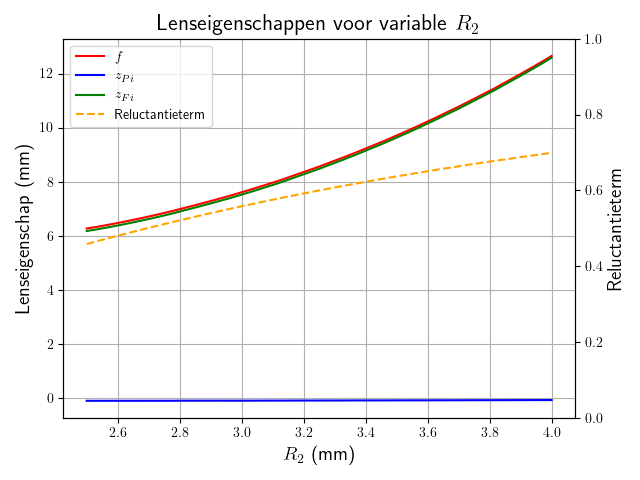
\includegraphics[width=\linewidth]{Images/variable_R_2.png}
        \caption{}
        \label{fig:variable_R_2}
    \end{subfigure}

    \vspace{0.5cm} 
    \begin{subfigure}[b]{0.45\linewidth}
        \centering
        
\includegraphics[width=\linewidth]{Images/variable_d.png}
        \caption{}
        \label{fig:variable_d}
    \end{subfigure}
    \hfill
    \begin{subfigure}[b]{0.45\linewidth}
        \centering
        
\includegraphics[width=\linewidth]{Images/variable_B_r.png}
        \caption{}
        \label{fig:variable_B_r}
    \end{subfigure}

    \caption{Plots van lenseigenschappen en reluctantieterm in functie van de geometrie van de lens. Deze plots geven een goed beeld van hoe de parameters aangepast kunnen worden om de lenseigenschappen naar wens te optimaliseren. Naast de reluctantieterm moet er ook rekening gehouden worden met de maximale fluxdichtheid in de poolschoenen, welke niet te hoog mag zijn om saturatie-effecten te voorkomen.}
    \label{fig:prop_grid_2x2}
\end{figure}

\begin{figure}[H]
    \centering
    
\includegraphics[width=0.45\linewidth]{Images/variable_T.png}
    \caption{Plot van de lenseigenschappen in functie van de versnelspanning $\Phi$. De afgeleiden van de lenseigenschappen naar de versnelspanning geven een maat voor de chromatische aberratie.}
    \label{fig:variable_T}
\end{figure}

We impementeren een gelijkaardige functie om ook de aberratiecoëfficiënten $D$ en $C_M$ in functie van de lensparameters $R_1$, $R_2$, $d_g$, en $B_r$ te bepalen. Zoals eerder vermeld zijn $D$ en $C_M$ afhankelijk van de objectafstand $z_0$, dus om een correcte vergelijking tussen verschillende lensiegenschappen te maken, houden we de objectafstand constant op $z_0=25\mathrm{mm}$, wat een typicshe afstand is bij een focales lengtes waarbij we werken ()$f\sim 10\mathrm{mm}$). Grafieken van de aberratiecoëfficiënten in functie van de lensparameters worden getoond op Figuur \ref{fig:ab_grid_2x2}.
\begin{figure}[H]
    \centering

    \begin{subfigure}[b]{0.45\linewidth}
        \centering
        
\includegraphics[width=\linewidth]{Images/variable_R_1_ab.png}
        \caption{}
        \label{fig:variable_R_1_ab}
    \end{subfigure}
    \hfill
    \begin{subfigure}[b]{0.45\linewidth}
        \centering
        
\includegraphics[width=\linewidth]{Images/variable_R_2_ab.png}
        \caption{}
        \label{fig:variable_R_2_ab}
    \end{subfigure}

    \vspace{0.5cm} 
    \begin{subfigure}[b]{0.45\linewidth}
        \centering
        
\includegraphics[width=\linewidth]{Images/variable_d_ab.png}
        \caption{}
        \label{fig:variable_d_ab}
    \end{subfigure}
    \hfill
    \begin{subfigure}[b]{0.45\linewidth}
        \centering
        
\includegraphics[width=\linewidth]{Images/variable_B_r_ab.png}
        \caption{}
        \label{fig:variable_B_r_ab}
    \end{subfigure}

    \caption{Plots van aberratiecoëfficiënten $D$ en $C_M$ in functie van de geometrie van de lens bij $z_0=25\mathrm{mm}$. Deze plots geven een goed beeld van hoe de parameters aangepast kunnen worden om de aberratiecoëfficiënten te minimaliseren.}
    \label{fig:ab_grid_2x2}
\end{figure}
Met deze hulpmiddelen kunnen we een geschikte set lensparameters kiezen die een optimale combinatie geeft van gewenste lenseigenschappen, klein demagnetiserend veld en minimale aberratiecoëfficiënten. We hebben gekozen voor de volgende lensparameters:
\begin{table}[H]
\centering
\begin{tabular}{@{}cl@{}}
\toprule
Lensparameter                     & \multicolumn{1}{c}{Waarde}  \\ \midrule
\multicolumn{1}{|c|}{$R_1$}        & \multicolumn{1}{c|}{$0.8\mathrm{mm}$}  \\ \midrule
\multicolumn{1}{|c|}{$R_2$}        & \multicolumn{1}{c|}{$3.25\mathrm{mm}$} \\ \midrule
\multicolumn{1}{|c|}{$d_g$}        & \multicolumn{1}{c|}{$0.8\mathrm{mm}$}  \\ \midrule
\multicolumn{1}{|c|}{$R_{1, m}$} & \multicolumn{1}{c|}{$4.5\mathrm{mm}$}  \\ \midrule
\multicolumn{1}{|c|}{$R_{2, m}$} & \multicolumn{1}{c|}{$6\mathrm{mm}$}    \\ \midrule
\multicolumn{1}{|c|}{$d_m$}        & \multicolumn{1}{c|}{$2\mathrm{mm}$}    \\ \midrule
\multicolumn{1}{|c|}{$B_r$}        & \multicolumn{1}{c|}{$1.17\mathrm{T}$} \\ \midrule
\end{tabular}
\caption{Gekozen lensparameters die een optimale lenswerking geven. We gebruiken een N35 graad NdfeB magneet, die een remanent veld van ongeveer $1.17\mathrm{T}$ heeft.}\label{tab:lens_parameters}
\end{table}
In de tabel staat er een enkele waarde voor het remanent veld, maar zoals eerder vermeld moeten we in feite heel de $\mathrm{BH}$-curve in rekening nemen. Deze hangt af van de graad van de magneet die we gebruiken. De ringmagneten werden geleverd door \textit{Magnet Outlet} \cite{Magnet_Outlet}. De gebruikte magneet is van de graad N35, maar jammer genoeg is er geen datasheet met alle specificaties van de magneet beschikbaar \cite{Magnet_Grade}. We gebruiken daarom de $\mathrm{BH}$-curve getoond op Figuur \ref{fig:BH_curve_NdFeB} bij het bepalen van de lenseigenschappen. De gekozen lensparameters geven aanleiding tot de volgende lenseigenschappen:
\begin{table}[H]
\centering
\begin{tabular}{@{}cl@{}}
\toprule
Lenseigenschap                     & \multicolumn{1}{c}{Waarde}  \\ \midrule
\multicolumn{1}{|c|}{$f$}        & \multicolumn{1}{c|}{$11.437\mathrm{mm}$}  \\ \midrule
\multicolumn{1}{|c|}{$z_{Pi}$}        & \multicolumn{1}{c|}{$-0.060\mathrm{mm}$} \\ \midrule
\multicolumn{1}{|c|}{$z_{Fi}$}        & \multicolumn{1}{c|}{$11.377\mathrm{mm}$}  \\ \midrule
\multicolumn{1}{|c|}{$P_{ci}$} & \multicolumn{1}{c|}{$2.575$}  \\ \midrule
\multicolumn{1}{|c|}{$B_{max}$} & \multicolumn{1}{c|}{$1.120\mathrm{T}$}    \\ \midrule
\multicolumn{1}{|c|}{$D$}        & \multicolumn{1}{c|}{$0.994\mathrm{mm}^{-2}$}    \\ \midrule
\multicolumn{1}{|c|}{$C_M$}        & \multicolumn{1}{c|}{$0.840$} \\ \midrule
\end{tabular}
\caption{Lenseigenschappen voor de gekozen lensparameters.}\label{tab:lens_properties}
\end{table}

Deze lenseigenschappen voldoen aan onze eisen. De lens is bij benadering een dunne lens met een focale lengte die voldoende kort is voor de MIRA SEM. Het demagnetiserend veld is niet te groot en de maximale fluxdichtheid in de poolschoenen is voldoende klein zodat we ons nog steeds in het lineair gebied van de $\mathrm{BH}$-curve op Figuur \ref{fig:BH_curve_ASI1018} bevinden. De aberratiecoëfficiënten $C_M$ is ook vergelijkbaar met typische waarden voor bruikbare elektronenlenzen. De coëfficiënt $D$ is echter redelijk groot vergeleken met literatuurwaarden. Het is echter zeer moeilijk om deze aberratiecoëfficienten nog kleiner te maken. Als we kijken naar Figuren \ref{fig:ab_grid_2x2} en \ref{fig:prop_grid_2x2}, dan zien we dat het veranderen van een van de lensparameters om $D$ te verkleinen steeds ongewenste neveneffecten heeft. Het vergroten van $R_1$ zorgt voor een kleinere focale lengte en een grotere fluxdichtheid in de poolschoenen. Ook het vergtoten van $R_2$ zal $f$ doen toenemen, en verkleint de afstand tussen de buitenkant van de poolschoenen en de binnenkant van de magneet waardoor de kans op een kortsluiting in het circuit groter is. Het vergroten van $d_g$ tot voorbij het maxima van $D$ geeft dan weer een te kleine $P_{ci}$ en een zwakkere magneet gebruiken zodat $B_r$ verkleint geeft ook een te lange focale lengte. Om deze redenen beargumenteren we dat dit de ideale set parameters is ook als is $D$ groot t.o.v. typische waarden uit de literatuur. Bovendien kunnen we de distorie op andere manieren experimenteel minimaliseren, hierover meer in hoofdstuk \ref{ch:karakterisatie}.\\

Eens we deze parameters hebben vastgelegd, moeten we een driedimensionaal model van de lens maken zodat de onderdelen door een CNC-service geproduceerd kunnen worden. We kiezen ervoor om het ontwerp in FreeCAD te maken. Dit kunnen we eenvoudig doen door een 2D sketch van een doorsnede van de lens met de gekozen afmetingen te maken, en vervolgens met de \textit{Revolution} functie van het programma een cilindrisch symmetrisch onderdeel op basis van de sketch te maken. Figuur \ref{fig:FreeCAD_2D} toont de 2D sketch met de afmetingen en enkele screenshots van het driedimensionaal model van de poolschoenen. We zorgen ervoor dat de poolschoen zo min mogelijk scherpe hoeken heeft, zodat het magnetisch veld nergens aan de buitenkant concentreert of weglekt. 
\color{red} Vervangen door technische tekeningen? \color{black}
\begin{figure}[H]
    \centering
    \begin{subfigure}[b]{0.4\linewidth}
        \centering
        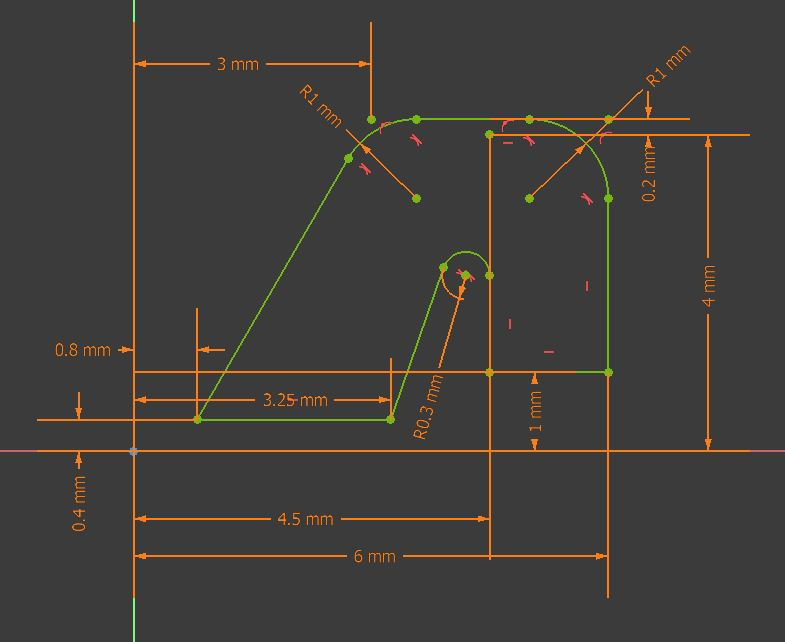
\includegraphics[width=\linewidth]{Images/FreeCAD_2D.JPG}
        \caption{}
        \label{fig:FreeCAD_2D}
    \end{subfigure}
    \hfill
    \begin{subfigure}[b]{0.4\linewidth}
        \centering
        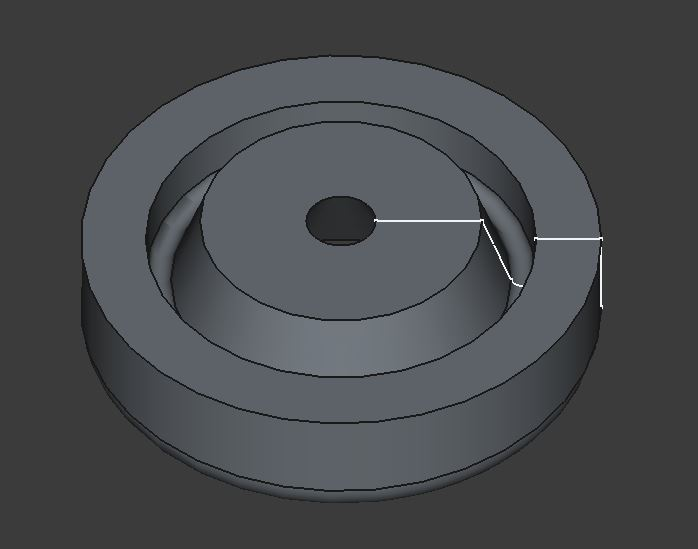
\includegraphics[width=\linewidth]{Images/FreeCAD_3D_1.JPG}
        \caption{}
        \label{fig:FreeCAD_3D_1}
    \end{subfigure}

    \vspace{0.5cm}

    \begin{subfigure}[b]{0.4\linewidth}
        \centering
        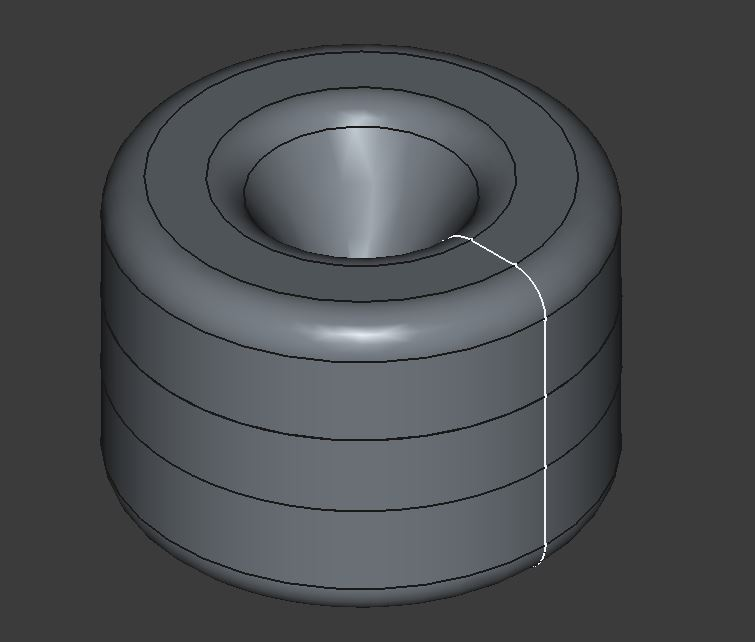
\includegraphics[width=\linewidth]{Images/FreeCAD_3D_2.JPG}
        \caption{}
        \label{fig:FreeCAD_3D_2}
    \end{subfigure}
    \hfill
    \begin{subfigure}[b]{0.4\linewidth}
        \centering
        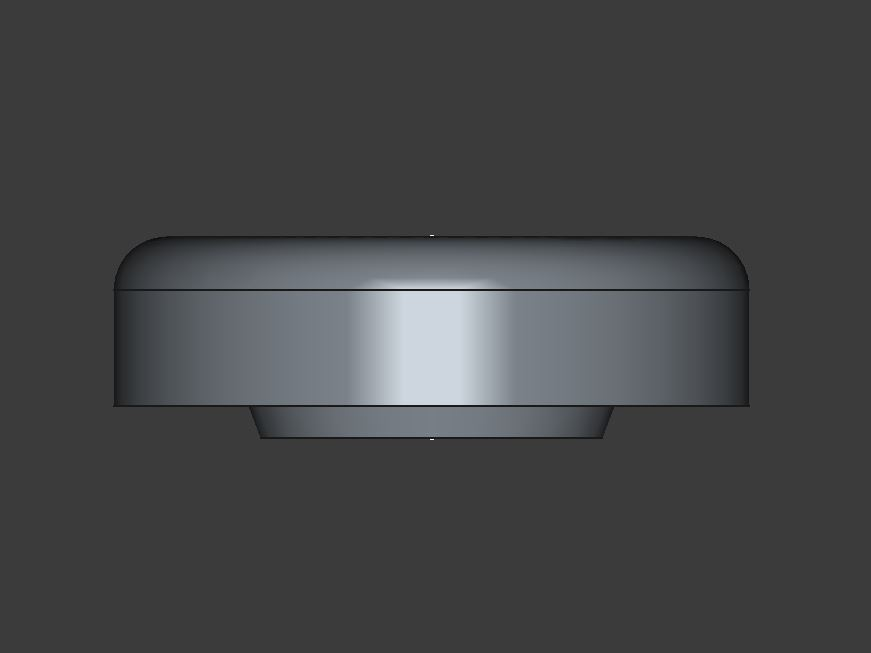
\includegraphics[width=\linewidth]{Images/FreeCAD_3D_4.JPG}
        \caption{}
        \label{fig:FreeCAD_3D_4}
    \end{subfigure}

    \caption{Verschillende aanzichten en een 2D sketch van het ontwerp van de poolschoenen in FreeCAD.}
    \label{fig:FreeCAD_grid_2x2}
\end{figure}

Deze stepfile hebben we opgestuurd naar de CNC-service \textit{Protolabs Network} \cite{Hubs}. We hebben de poolschoenen laten maken in ASI1018 waarbij het oppervlak gepassiveerd wordt. Dit is een behandeling met $HNO_3$ waarbij er een dunne laag metaaloxide aan de buitenkant van het ASI1018 gevormd wordt \cite{MALLER199828}. Op deze manier wordt er voorkomen dat het materiaal begint te roesten, wat de permeabiliteit kan veranderen of oppervlakte-effecten veroorzaakt welke het magnetisch veld zullen beïnvloeden.

\begin{tcolorbox}[colback=blue!10!white,colframe=blue!75!black,title=Realisatie objectief 6]
    De optimale lensparameters worden bepaald door een trial-and-errorproces ondersteund door variatie-plots waarbij telkens 1 parameter wordt aangepast. De Python toolbox werd hiervoor uitgebreid met functies die de lenseigenschappen, aberratiecoëfficiënten en permeantiecoëfficiënt voor een variabele lensparameter berekenen en plotten. Gebruik makend van deze functieswerd er een set lensparameters vastgelegd die maximaal voldoet aan de opgestelde criteria voor de lenswerking.  Enkel de distortieaberratiecoëfficiënt overschrijdt de gewenste waarde met een factor~$2$; een alternatieve configuratie die dit verbetert zonder de overige lenseigenschappen te benadelen, werd niet gevonden. Op basis van de meest optimale lensparameters werd een driedimensionale geometrie voor de lens in FreeCAD ontworpen. 
\end{tcolorbox}

\section{Karakterisatie in de microscoop}\label{ch:karakterisatie}

\section{Experimentele validatie focale lengte}

\subsection{Mesh shadowgraph methode}
Om de focale lengte en eventueel andere lenseigenschappen van de lens te bepalen gebruiken we een aangepaste versie van de \textit{rear mesh shadowgraph methode} beschreven in \cite{meshshadowgraphs}. Het algemene principe van deze methode bestaat er in om met behulp van de lens een divergerende elektronenbundel te maken. De focale lengte kan dan worden afgeleid door te meten hoe divergent deze elektronenbundel juist is. Concreet kunnen we dit meten door een fijnmazig rooster (mesh grid) achter de lens in de divergerende bundel te plaatsen, zodat er een uitvergroot schaduwbeeld op de detector wordt geworpen. De vergroting van het schaduwbeeld is dan een maat voor de divergentie van de elektronenbundel. Hieronder werken we enkele gevallen wiskundig uit.\\

Een van de methodes beschreven in \cite{meshshadowgraphs} maakt gebruik van een puntbron op de optische as die we een afstand $z>f$ van de lens plaatsen. We veronderstellen dat we een dunne lens gebruiken, waardoor we de dunne lensformule kunnen gebruiken:
\begin{equation}\label{eq:thin_lens_formula}
    \frac{1}{f}=\frac{1}{z}+\frac{1}{z'}
\end{equation}
De puntbron wordt dan achter de lens afgebeeld op een afstand $z'>f$ van de lens. We plaatsen nu een grid met een nauwkeurig gekende periode van $e_1$ op een afstand $b$ van de lens, waarbij $b>z'$ zodat de elektronenbundel wordt gefocusseerd voor het grid. Op een afstand $d$ van het grid plaatsen we een elektronendetector. Het beeld van de puntbron op $z'$ veroorzaakt nu een divergerende elektronenbundel die een uitvergroot schaduwbeeld van het grid op de detector werpt. De opstelling wordt getoond op Figuur \ref{fig:rear_mesh_shadowgraph}.
\begin{figure}[H]
    \centering
    
\includegraphics[width=0.6\linewidth]{Images/rear_mesh_shadowgraph.png}
    \caption{Rear mesh shadowgraph methode voor een puntbron voor het focaalvlak van de lens. Door de vergroting $M=\frac{E}{e}$ te meten is het mogelijk om het beeldpunt $z'$ en de focale lengte $f$ te bepalen.}
    \label{fig:rear_mesh_shadowgraph}
\end{figure}
Op het detectorbeeld meten we de grootte van 1 of meerdere afgebeeldde roosteropeningen, welke we aanduiden met $E$. De werkelijke afmeting van de roosteropeningen duiden we aan met $e=ne_1$ met $n$ het aantal roosteropeningen dat we beschouwen. De vergroting van het schaduwbeeld is gelijk aan $M\frac{E}{e}$. Uit gelijkvormigheid van driehoeken volgt dan:
\begin{equation}
    \frac{c}{e}=\frac{c+d}{E}\Leftrightarrow\frac{E}{e}=M=1+\frac{d}{c}
\end{equation}
Dit kunnen we omvormen om $c$ te vinden:
\begin{equation}
    c=\frac{d}{M-1}
\end{equation}
Hiermee kunnen we eenvoudig de beeldafstand $z'$ bepalen:
\begin{equation}\label{eq:image_dist_real}
    z'=b-c=b-\frac{d}{M-1}
\end{equation}
Met de beeldafstand kunnen we de focaalafstand berekenen door vergelijking \ref{eq:thin_lens_formula} om te vormen. In het experiment dat we in deze thesis zullen uitvoeren passen we de voorgaande methode op twee manieren aanpassen, welke hieronder in meer detail worden uitgelegd.\\

Het is mogelijk dat de werkelijke focale lengte van de lens groter is dan de voorspelde focale lengte, waardoor de initiële puntbron achter het voorste focaalvlak van de lens ligt. In dat geval wordt er geen reëel beeld achter de lens, maar een virtueel beeld voor de lens gevormd. Dit wordt getoond op Figuur \ref{fig:rear_mesh_shadowgraph_virtual}.
\begin{figure}[H]
    \centering
    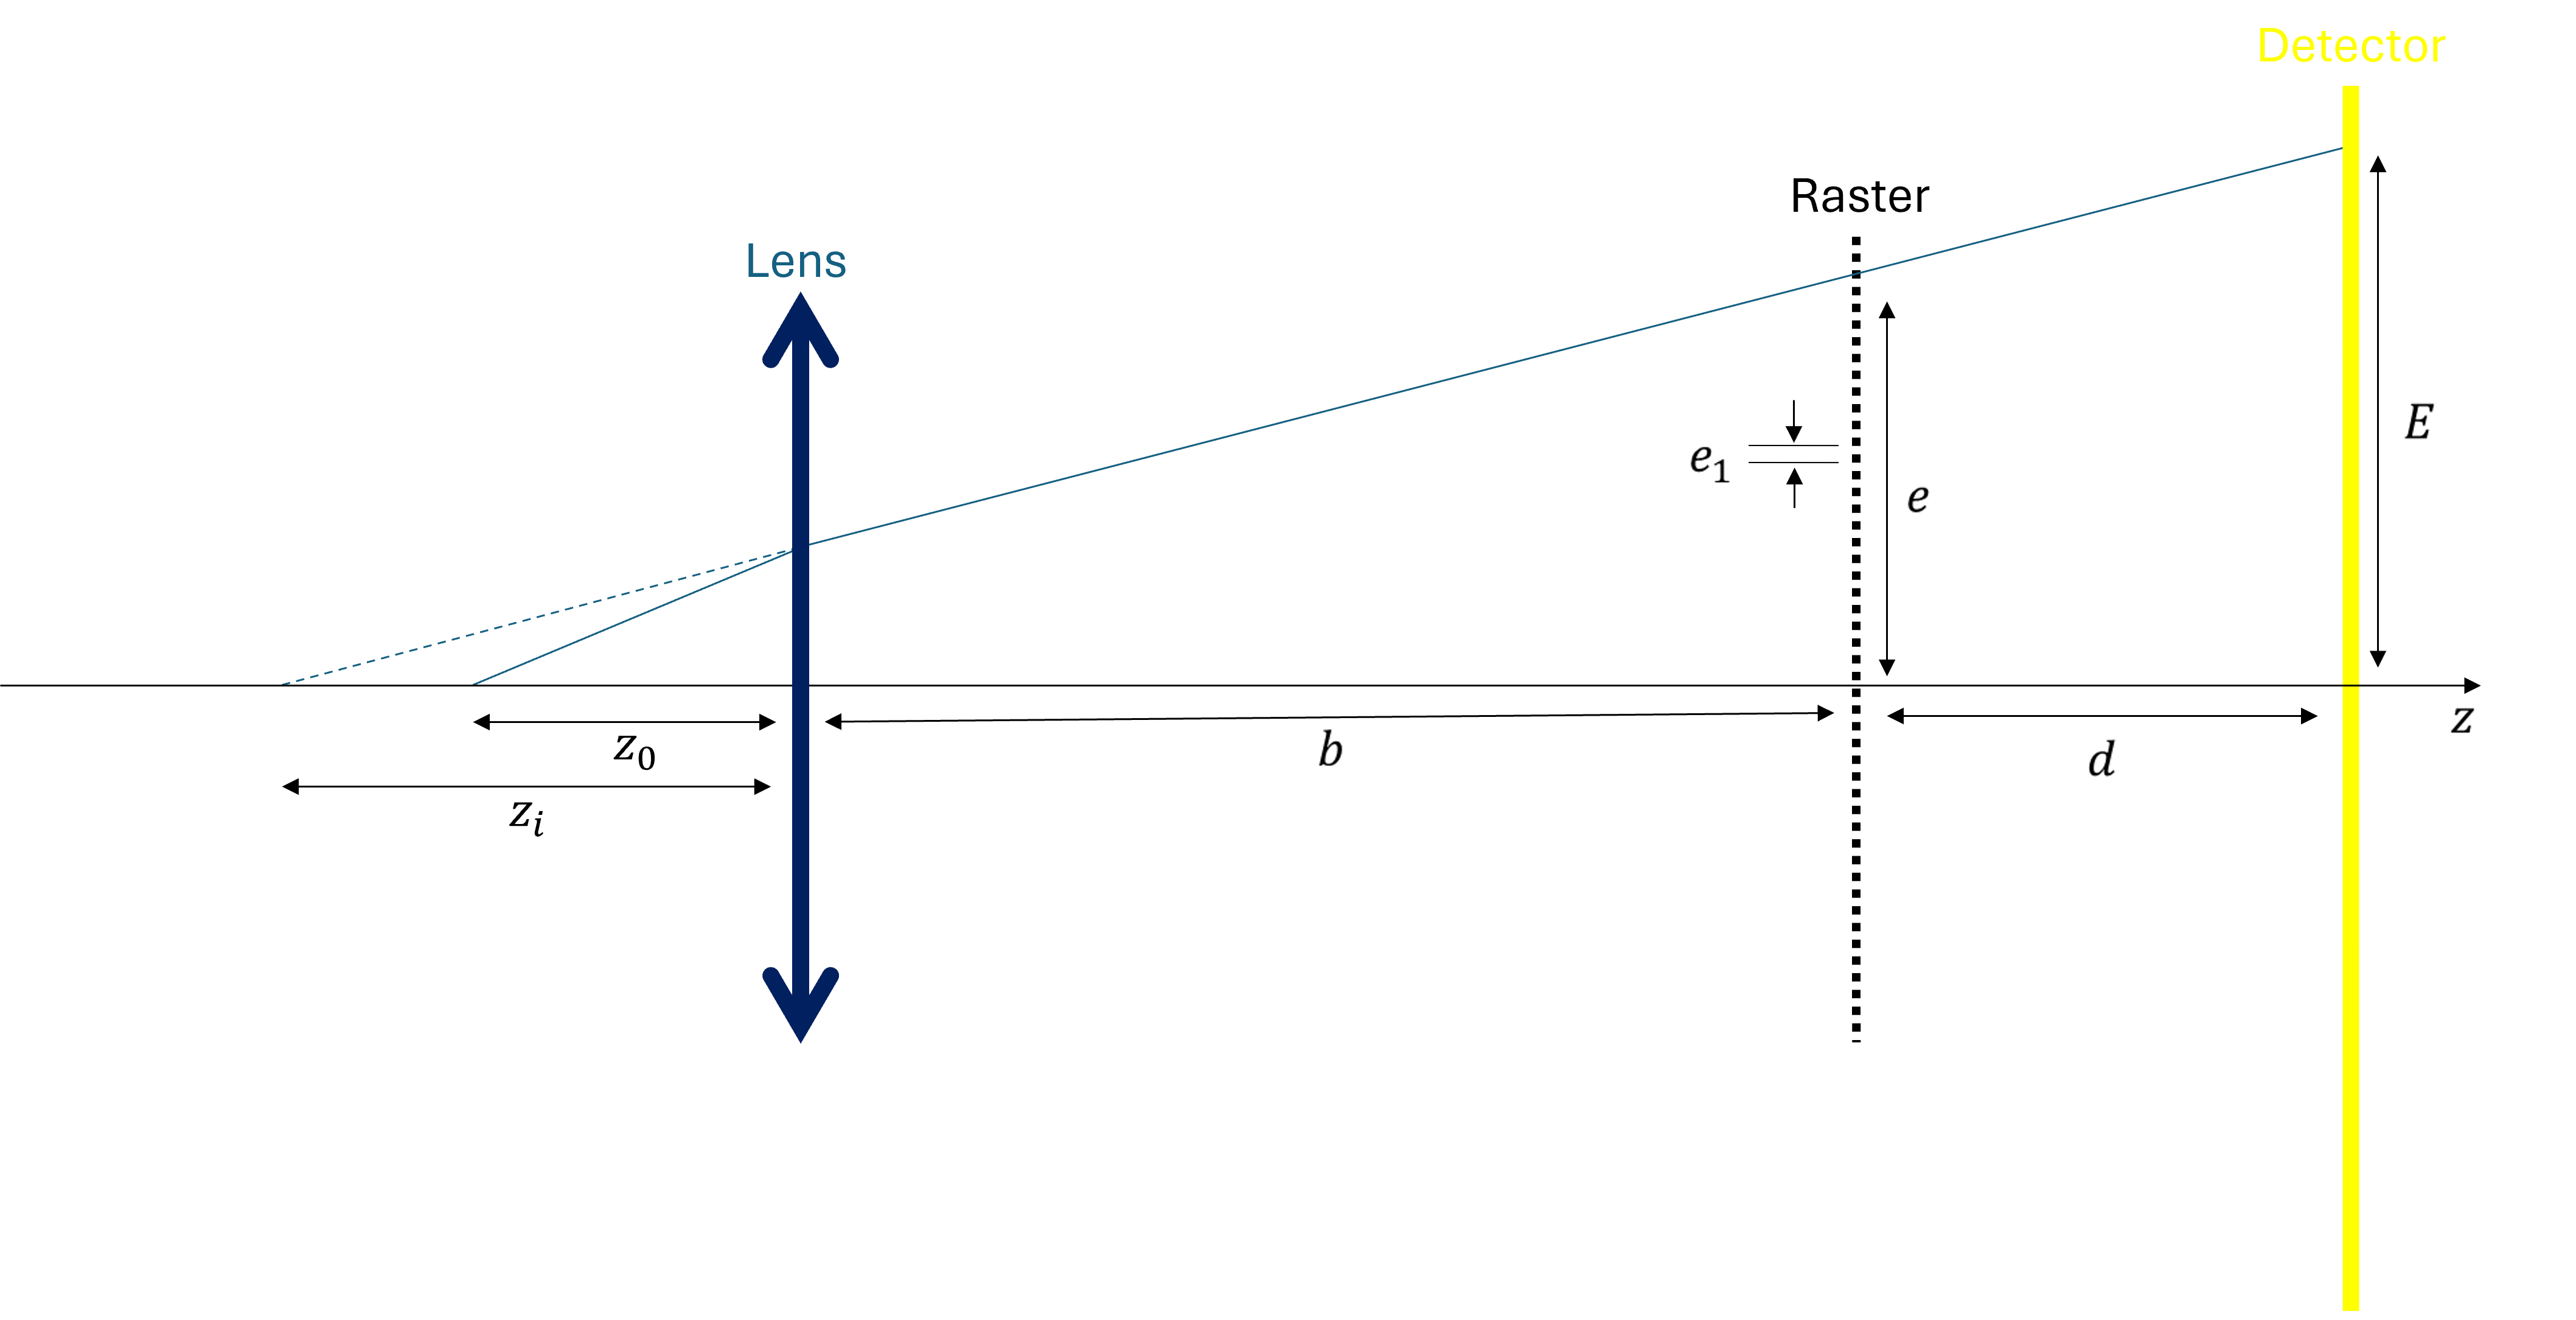
\includegraphics[width=0.6\linewidth]{Images/rear_mesh_shadowgraph_virtual_image.png}
    \caption{Rear mesh shadowgraph methode voor een puntbron achter het focaalvlak van de lens. De elektronenbundel wordt nu niet gefocusseerd in een punt, maar de elektronenbundel is nog steeds divergerend wat een vergroting $M>1$ geeft. }
    \label{fig:rear_mesh_shadowgraph_virtual}
\end{figure}
Het is met deze opstelling nog steeds mogelijk om op deze manier de focale lengte te berekenen. Opnieuw vinden we uit gelijkvormigheid dat:
\begin{equation}
    \frac{e}{z'+b}=\frac{E}{z'+c+d}\Leftrightarrow\frac{E}{e}=M=1+\frac{d}{z'+b}
\end{equation}
Dit omvormen naar $z'$ geeft:
\begin{equation}
    z'=b-\frac{d}{M-1}
\end{equation}

Merk op dat dit exact dezelfde formule geeft als bij een reëel beeld (\ref{eq:image_dist_real}). Opnieuw gebruiken we \ref{eq:thin_lens_formula} om $f$ te berekenen.\\

Een mogelijke manier om de mesh shadowgraph methode te vereenvoudigen is om een parallelle i.p.v. een conische elektronenbundel op de lens in te sturen. In dat geval is $z=\infty$, waardoor uit \ref{eq:thin_lens_formula} volgt dat $z'=f$. We kunnen dezelfde procedure als in de originele methode gebruiken om $c$ te bepalen, maar nu kunnen we de focale lengte rechtstreeks bepalen uit $f=b-c$. Figuur \ref{fig:rear_mesh_shadowgraph_parallel} toont de opstelling in dit geval.
\begin{figure}[H]
    \centering
    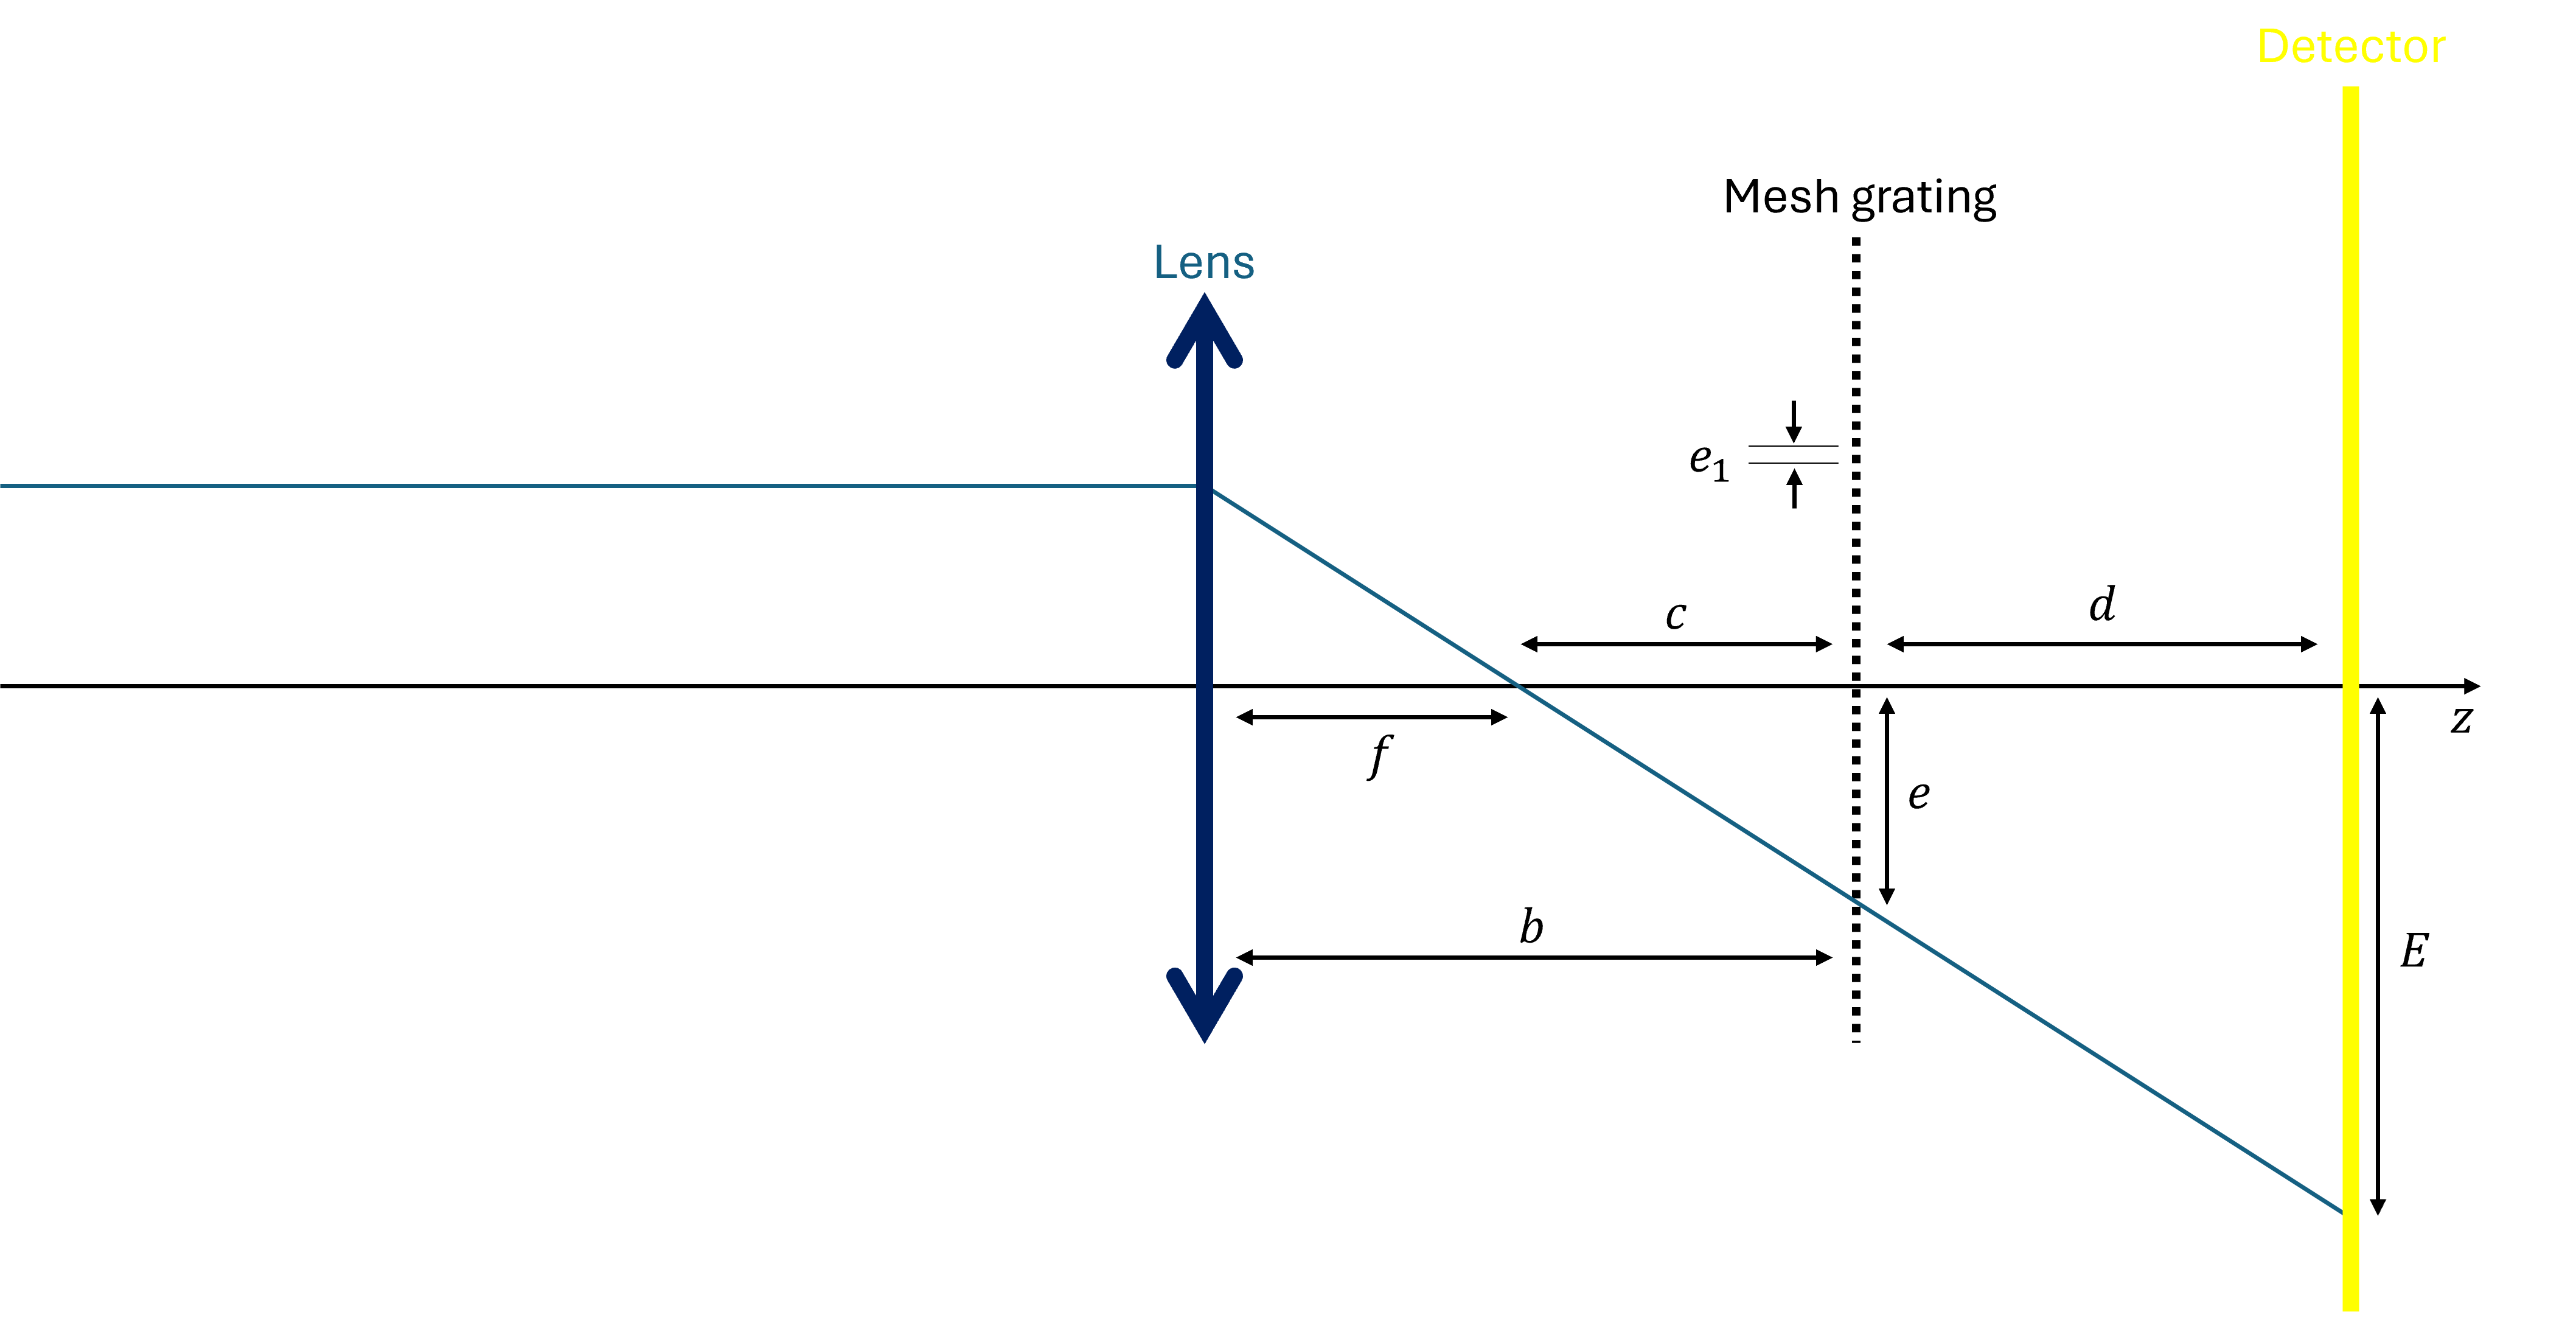
\includegraphics[width=0.6\linewidth]{Images/rear_mesh_shadowgraph_parallel_beam.png}
    \caption{Rear mesh shadowgraph methode voor een parallelle bundel. Door het gebruik van een parallelle bundel worden de inkomende elektronenbundels door de lens gefocusseerd in het focaalvlak achter de lens, wat de bepaling van de focale lengte iets vereenvoudigt.}
    \label{fig:rear_mesh_shadowgraph_parallel}
\end{figure}
In principe kan deze methode ook uitgebreid worden om de chromatische en sferische aberratiecoëfficiënten van de lens te berekenen. De sferische aberratiecoëfficiënt kan worden afgeleid door de afgebeeldde grootte van de individuele roosteropeningen uit te zetten in functie van de afstand tot de optische as van het systeem. Immers, hoe verder de roosteropening zich van de optische as bevindt, hoe groter de hoek $\alpha$ tussen de elektronen en de optische as. Sferische aberratie kan worden uitgedrukt als $\Delta z' = -C_s \alpha^2$, dus door $z'$ voor verschillende waarden van $\alpha$ te berekenen kunnen we de sferische aberratiecoëfficiënt $C_s$ fitten. De chromatische aberratie kunnen we berekenen door de versnelspanning van de micrscoop aan te passen. De chromatische aberratiecoëfficiënt $C_f$ kunnen we dan berekenen uit $\frac{\Delta f}{f}=C_f\frac{\Delta V}{V}$.

\subsection{Monte Carlo simulatie van het experiment}


\chapter{Vooruitzicht}\label{ch:vooruitzicht}

\chapter{Besluit}\label{ch:besluit}

\bibliographystyle{abbrv}
\bibliography{bibliography}   % your .bib filename without .bib extension

\end{document}


\endinput
%%
%% End of file `uantwerpenbamathesis-example.tex'.
